\documentclass{article}
\usepackage[utf8]{inputenc}
\usepackage{geometry}[margin=0.5in]
\usepackage{amsfonts}
\usepackage{amsmath}
\usepackage{amssymb}
\usepackage{physics}
\usepackage{braket}
\usepackage{amsthm}
\usepackage[english]{babel}
\usepackage{graphicx}
\usepackage{float}
\usepackage{mathtools}
\usepackage{algorithm2e}
\usepackage{hyperref}
\usepackage[title]{appendix}
\usepackage{chngcntr}

\theoremstyle{definition}
\newtheorem{definition}{Definition}[section]
\title{Causal Effects on Networks Need to Account for Effect Modification by Network Structure}
\author{Nico D'Angelo, Sam Bessey , Kareem Carr,..., Brandon Marshall,  Ashley Buchanan,  Eleanor J Murray }
\date{}

\begin{document}

\maketitle

\section{Introduction}
Transmission of infection, knowledge, behavior, or other features between individuals is a challenge in estimating causal effects of population interventions. Causal effect estimation relies on the ability to validly estimate unobserved counterfactual information for comparison. In the potential or counterfactual outcomes framework, this typically relies on the Stable Unit Treatment Value Assumption, or SUTVA, which assumes that the individuals under study are independent from and exchangeable with one another. Transmission inherently violates SUTVA, by creating a dependence between the exposure of one individual and the counterfactual outcomes of other individuals. Several paradigms have been proposed for defining causal effects in the presence of transmission, of which the Dependent Happenings paradigm of Halloran et al  \cite{halloran_study_1991} is the most widely used. However, this paradigm of effects has largely been specified in the context of group-level comparisons from observational or randomized trial data. When applied to network-based simulation models, additional concerns arise which have not been previously addressed. 

Here, we begin by outlining the causal estimands available in the setting of transmission, or spillover, and then describe how these estimands should be extended when network effects are of interest. We propose two separate sets of estimands which may be of interest, one for when the empirical network is known and one for when only the network characteristics or distribution are known. We describe theoretically the importance of these estimands in obtaining valid effects, as well as consequences for simulation model design. Finally, we provide a simple simulated example which demonstrates the potential magnitude of bias that can occur when using inappropriate simulation approaches.

\section{Defining Causal Estimands under Spillover}
In the Dependent Happenings paradigm, causal effects under transmission, also called spillover, can be grouped into four major categories. Within each category, there exists a causal effect surface across the possible community exposure levels. Briefly, these four categories are:
\begin{definition}[Direct Effect]The direct effect is the average benefit or harm experienced by each individual if they received the exposure versus if they had not, within their community context. This effect includes any changes over time to the community context, and is conditional on the community context in which it is measured. 
%Need example%
\end{definition}
\begin{definition}[Spillover Effect] The spillover effect is the average benefit or harm to each unexposed individual in a community if some individuals in the community had received exposure versus if those individuals had not received exposure. This effect describes the impact of changing community context and is conditional on the particular patterns of community exposure under comparison.
\end{definition}
\begin{definition}[Composite effect]The composite effect is the average benefit or harm experienced by individuals if they had received exposure versus if neither they nor anyone else in their community had received exposure.
\end{definition}
\begin{definition}[Overall effect] The overall effect is the average benefit or harm to whole community, if some or all individuals had received the exposure versus if fewer or no individuals had received exposure. 
\end{definition}


\begin{figure}[H]
    \centering
    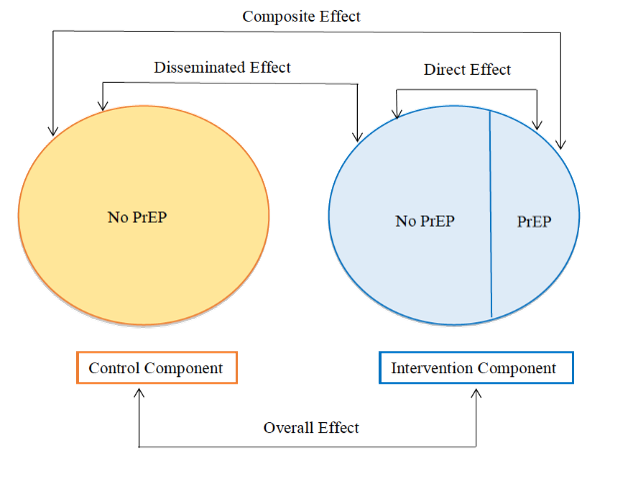
\includegraphics{Figures/figure1.png}
    \caption{The causal effects of interest for PrEP use in a sexual contact network.}
    \label{fig:1}
\end{figure}
Of these, the Direct Effect is generally the easiest to estimate in the context of a randomized trial. When the exposure is experimental and not available outside of the trial context, and the trial participants are not in contact with one another, then the Direct Effect also approximates the Composite Effect. The Direct Effect is also often of interest in observational studies where the prevalence of exposure is fixed in a given population over the course of the study.

Spillover, Composite, and Overall Effects are more difficult to estimate because the exposure context is itself part of the effect definition. More precisely, these can be treated as effect estimand surfaces where the value of the estimand is conditional on a specific exposure, interference, and contact pattern, rather than point estimands. 

In community-level randomized trials, cluster randomized trials, or two-stage randomized trials, all four effect categories can typically be estimated, assuming sufficient data are collected. In these cases, the exposure contexts are fixed to a small number of options, typically including a 'zero exposure' context. This simplifies the estimation of effect surface. Recently, attempts have been made to conceptualize network simulation models as emulations of these trials  \cite{murray_emulating_2021} in order to clarify the causal estimands available from these models. Here, we consider the role of simulation uncertainty in the definition and estimation of these estimands.

\section{Question}
%\section{Motivation}
The Direct, Spillover, Composite, and Overall Effects all incorporate changes in the contact patterns of the network or network component into their definitions. As such, the central question of this investigation is: ``Does the way that counterfactuals and counterfactual contrasts are simulated affect the causal estimand that can be estimated and/or the assumptions that need to be made in order to get valid estimates of causal effects under interference?''
If so, which approaches, assumptions, and estimands are the best for what we actually want to learn, i.e., are the most interpretable and most relevant to interventions?
\section{Effect Modification Scenarios and Estimands of Interest}
The roles/effects that model components play may vary between different estimands of interest. The following subsections explore the effects of Network Structure/Generation and Treatment Assignment. 

In the following derivations, let $Y$ be the outcome of interest, $a,a*$ be counterfactuals of treatment strategy $A$, and $j$ be an identifier of a network.
\subsection{Effect of Network Structure}
The effect of network structure may depend on the estimand of interest. 

In observational data, we may estimate
\begin{equation}\label{eq:1}
    \mathbb{E}_{i}\left[Y_{i,j}^{a}-Y_{i,j}^{a*}\right],
\end{equation}
the expectation over individuals $i$ within the network $j$. If we have a particular network realization of interest, this comparison is estimating the average effect on that network $j$: 
\begin{equation}\label{eq:2}
    \mathbb{E}\left[Y^{a}_{i,j}-Y^{a*}_{i,j}|j\right],
\end{equation}

In simulated data, we may not be interested in any particular network, so we instead estimate
\begin{equation}\label{eq:3}
    \mathbb{E}\left[Y^{a}-Y^{a*}\right]=\mathbb{E}_{j}\left[\mathbb{E}\left[Y_{j}^{a}-Y_{j}^{a*} \vert j\right]\right],
\end{equation}
taking the expectation under treatment over all possible network structures considered. 
\subsubsection{Equivalence of Observational and Simulation Estimands}
We are also interested in determining whether the observational estimand in \ref{eq:1} is equal to the simulation estimand in \ref{eq:3}. If our contact network of interest is drawn at random from a specified distribution, and the true effect is expected to be identical (up to stochasticity) in all such networks, then the effect in any one network should approximate the effect in all networks.

In epidemiologic terms: If there is no effect modification by contact network structure, $j$, then we expect that the average effect across contact networks is the same as the average effect on a given contact network, hence the equivalence of \ref{eq:1}, \ref{eq:2} and the right-hand side of \ref{eq:3}:
\begin{equation}\label{eq:4}
      \mathbb{E}\left[Y_{i,j}^{a}-Y_{i,j}^{a*}\vert j\right]=\mathbb{E}\left[Y^{a}-Y^{a*}\right]=\mathbb{E}_{j}\left[\mathbb{E}\left[Y_{j}^{a}-Y_{j}^{a*}\vert j\right]\right].
\end{equation}
\subsection{Effect of Treatment Assignment}
\label{sec: Treat}
We are usually interested in treating only a subset of eligible individuals. Specifically, we want to prioritize those individuals who have at least one infectious contact. However, it is generally impossible to identify all such individuals. As such, the estimand must aggregate all possible treatment distributions and account for the heterogeneity of the treatment effect between those with and without infectious contacts.

Thus, while we are interested in estimating \ref{eq:1} from observational data, we are actually interested in estimating 
\begin{equation}\label{eq:5}
    \mathbb{E}_{\Set{a,a*   }}\left[\mathbb{E}\left[Y_{j}^{a}-Y_{j}^{a*}\right]\right],
\end{equation}
averaging over all ways that a treatment $A$ can applied to network $j$. That is, we take expectations over all individuals in a given network $j$, then over all treatments $a,a*$ of $A$ that can be applied to the network.

The estimand in \ref{eq:5} is also of interest in a simulation model since we don't preferentially apply either value of $A$. Simulation studies theoretically avoid the limiting assumption that the observed treatment scenario is representative by allowing for all possible combinations to be simulated. However, in practice the number of combinations is large and exhaustive simulation is computationally impractical.


For a single time point, let $N$ denote the number of uninfected individuals in the network, and $k <N$ denote the number of individuals in the network who will receive treatment. Then, there are $\binom{N}{k}$ unique network configurations.

Assume that $k$ is chosen at random from the $N$ uninfected individuals, and that $n<N$ of the uninfected individuals have an infectious contact. The expected number of unique network configurations  in which all treated individuals have no infectious contacts (and thus a contribution of 0 to the effect estimate) is then given by $\binom{N-n}{k}$. Then, the proportion of network configurations in which at least one treated individual has at least one infectious contact is 
\begin{equation}\label{eq:6}
    \frac{{\binom{N}{k}}-{\binom{N-n}{k}}}{{\binom{N}{k}}}=1-\left(1-\frac{k}{N}\right)^{n}.
\end{equation}
That is, the probability of at least one node $i$ assigned to treatment with at least one infectious contact for a given network structure $j$ and treatment assignment is:
\begin{equation}\label{eq:7}
    P \coloneqq \mathbb{P}\left(n_{i}=1 \vert k_{i}=1,j,a,a*\right)=1-\left(1-\frac{k}{N}\right)^{n}.
\end{equation}
Note that 
\begin{equation}\label{eq:8}
    \lim_{N \to \infty}P=\begin{cases}0 & k,n \text{ fixed} \\ 1 & k \to N \lor n \to N  \end{cases}
\end{equation}

\subsection{Effect of Network Regeneration}
\label{sec:Regen}
It is important to note that we often do not actually estimate \ref{eq:2}. If we are regenerating the network at each iteration of the simulation, then we are estimating \begin{equation}\label{eq:9}
    \mathbb{E}_{\Set{j,j*}}\left[\mathbb{E}\left[Y_{j}^{a}\right]-\mathbb{E}\left[Y_{j*}^{a*}\right]\right],
\end{equation} 
which is the average over the joint distribution of all combinations of network structures $j$ and $j*$ of the difference between the average potential outcome under treatment assignment $a$ with network structure $j$ and the average potential outcome under  treatment assignment $a*$ with network structure $j*$.

This raises the question of whether the network regeneration estimand in \ref{eq:9}  is equal to the network structure estimand from \ref{eq:2}. Recall that causal contrasts require that the counterfactuals being compared represent 2 possible counterfactual experiences of a single group. As such, if we are regenerating the network each time that we generate a counterfactual, then we need to assume that every network instance and every treatment represents a possible experience of the exact same individuals. 

But, in some networks an individual might be treated and have an infectious contact, while in others they may be treated and not have an infectious contact, or not be treated and have an infectious contact, or be treated and have no infectious contacts. If we did not explicitly average over all of these scenarios, we would need to assume constancy of counterfactuals across networks in addition to constancy of effects across networks. This is tantamount to assuming no effect modification for all possible treatment values, which requires no confounders of outcome by contact pattern or treatment.
%Mention randomization!
\subsubsection{A Note on Some Problems and Assumptions}

However, it is important to remember that the utility of modelling effects on networks comes from the ability to encode network structure/contact patterns as effect modifiers. In this particular context, not assigning treatment based on contact risk means that contact risk strongly affects infection risk. Also, assignment by contact risk would still allow for effect modification if limitations in identifying future contacts occur. Since it is often nearly impossible to perfectly identify future infectious contacts in advance, contact risk effect modification will occur whether or not treatment is applied.

A key assumption to keep in mind is that lack of effect modification requires that the effect estimate does not depend on who in each community does/does not get exposed. But, we know that there is heterogeneity in real contact patterns, and that Independence between contact patterns and exposure status does not usually hold. In particular, individuals usually choose exposure on the basis of perceived outcome risk. As such, the individual-level benefit of receiving a protective exposure will depend on whether that individual receives an infectious exposure. Thus, individual effects are not homogeneous and we must consider infectious exposure an effect modifier. Individual beliefs about the likelihood of an infectious exposure will also cause both infectious and protective exposures. Thus, infectious exposure is thus both a confounder and an effect modifier for the individual effect and this propagates to the overall effect. 
\subsubsection{Equivalence of Network Regeneration and Simulation Estimands}
We are then interested in whether the estimands in \ref{eq:9} and \ref{eq:2} are equivalent.

Having identified that the network structure $j$ is an effect modifier, we know it is possible that \begin{equation}
    \mathbb{E}_{j}\left[\mathbb{E}\left[Y_{j}^{a}-Y_{j}^{a*}\right]\right] \neq \mathbb{E}\left[Y_{j}^{a}-Y_{j}^{a*}\right],
\end{equation}
and that
\begin{equation}
    \mathbb{E}_{j}\left[\mathbb{E}\left[Y_{j}^{a}-Y_{j}^{a*}\right]\right]\neq  \mathbb{E}_{\Set{j,j*}}\left[\mathbb{E}\left[Y_{j}^{a}\right]-\mathbb{E}\left[Y_{j*}^{a*}\right]\right]. 
\end{equation}

But our analyses estimate either 
\begin{equation*}
\mathbb{E}\left[Y_{j}^{a}-Y_{j}^{a*}\right]    
\end{equation*}
or 
\begin{equation*}
    \mathbb{E}\left[Y_{j}^{a}\right]-\mathbb{E}\left[Y_{j*}^{a*}\right]
\end{equation*}
and then combine them across all runs.
\section{Goal}
An important goal of this investigation is then to identify valid approaches and assumptions for estimating $$\mathbb{E}\left[Y^{a}-Y^{a*}\right].$$

We first need to develop estimators and clarify the assumptions for identifying each of the expectations $$\mathbb{E}_{\Set{j,j*}}\left[\mathbb{E}\left[Y_{j}^{a}\right]-\mathbb{E}\left[Y_{j*}^{a*}\right]\right],$$ and
$$\mathbb{E}_{j}\left[\mathbb{E}\left[Y_{j}^{a}-Y_{j}^{a*}\right]\right]$$ expanding on the definitions of overall, composite, direct, and spillover effects.

We then create a simulated network with known effects.

Finally, we draw model parameters from that network and obtain estimates using standard methods (and any additional methods identified in the first step).
\section{Estimators}

\begin{figure}[H]
    \centering
    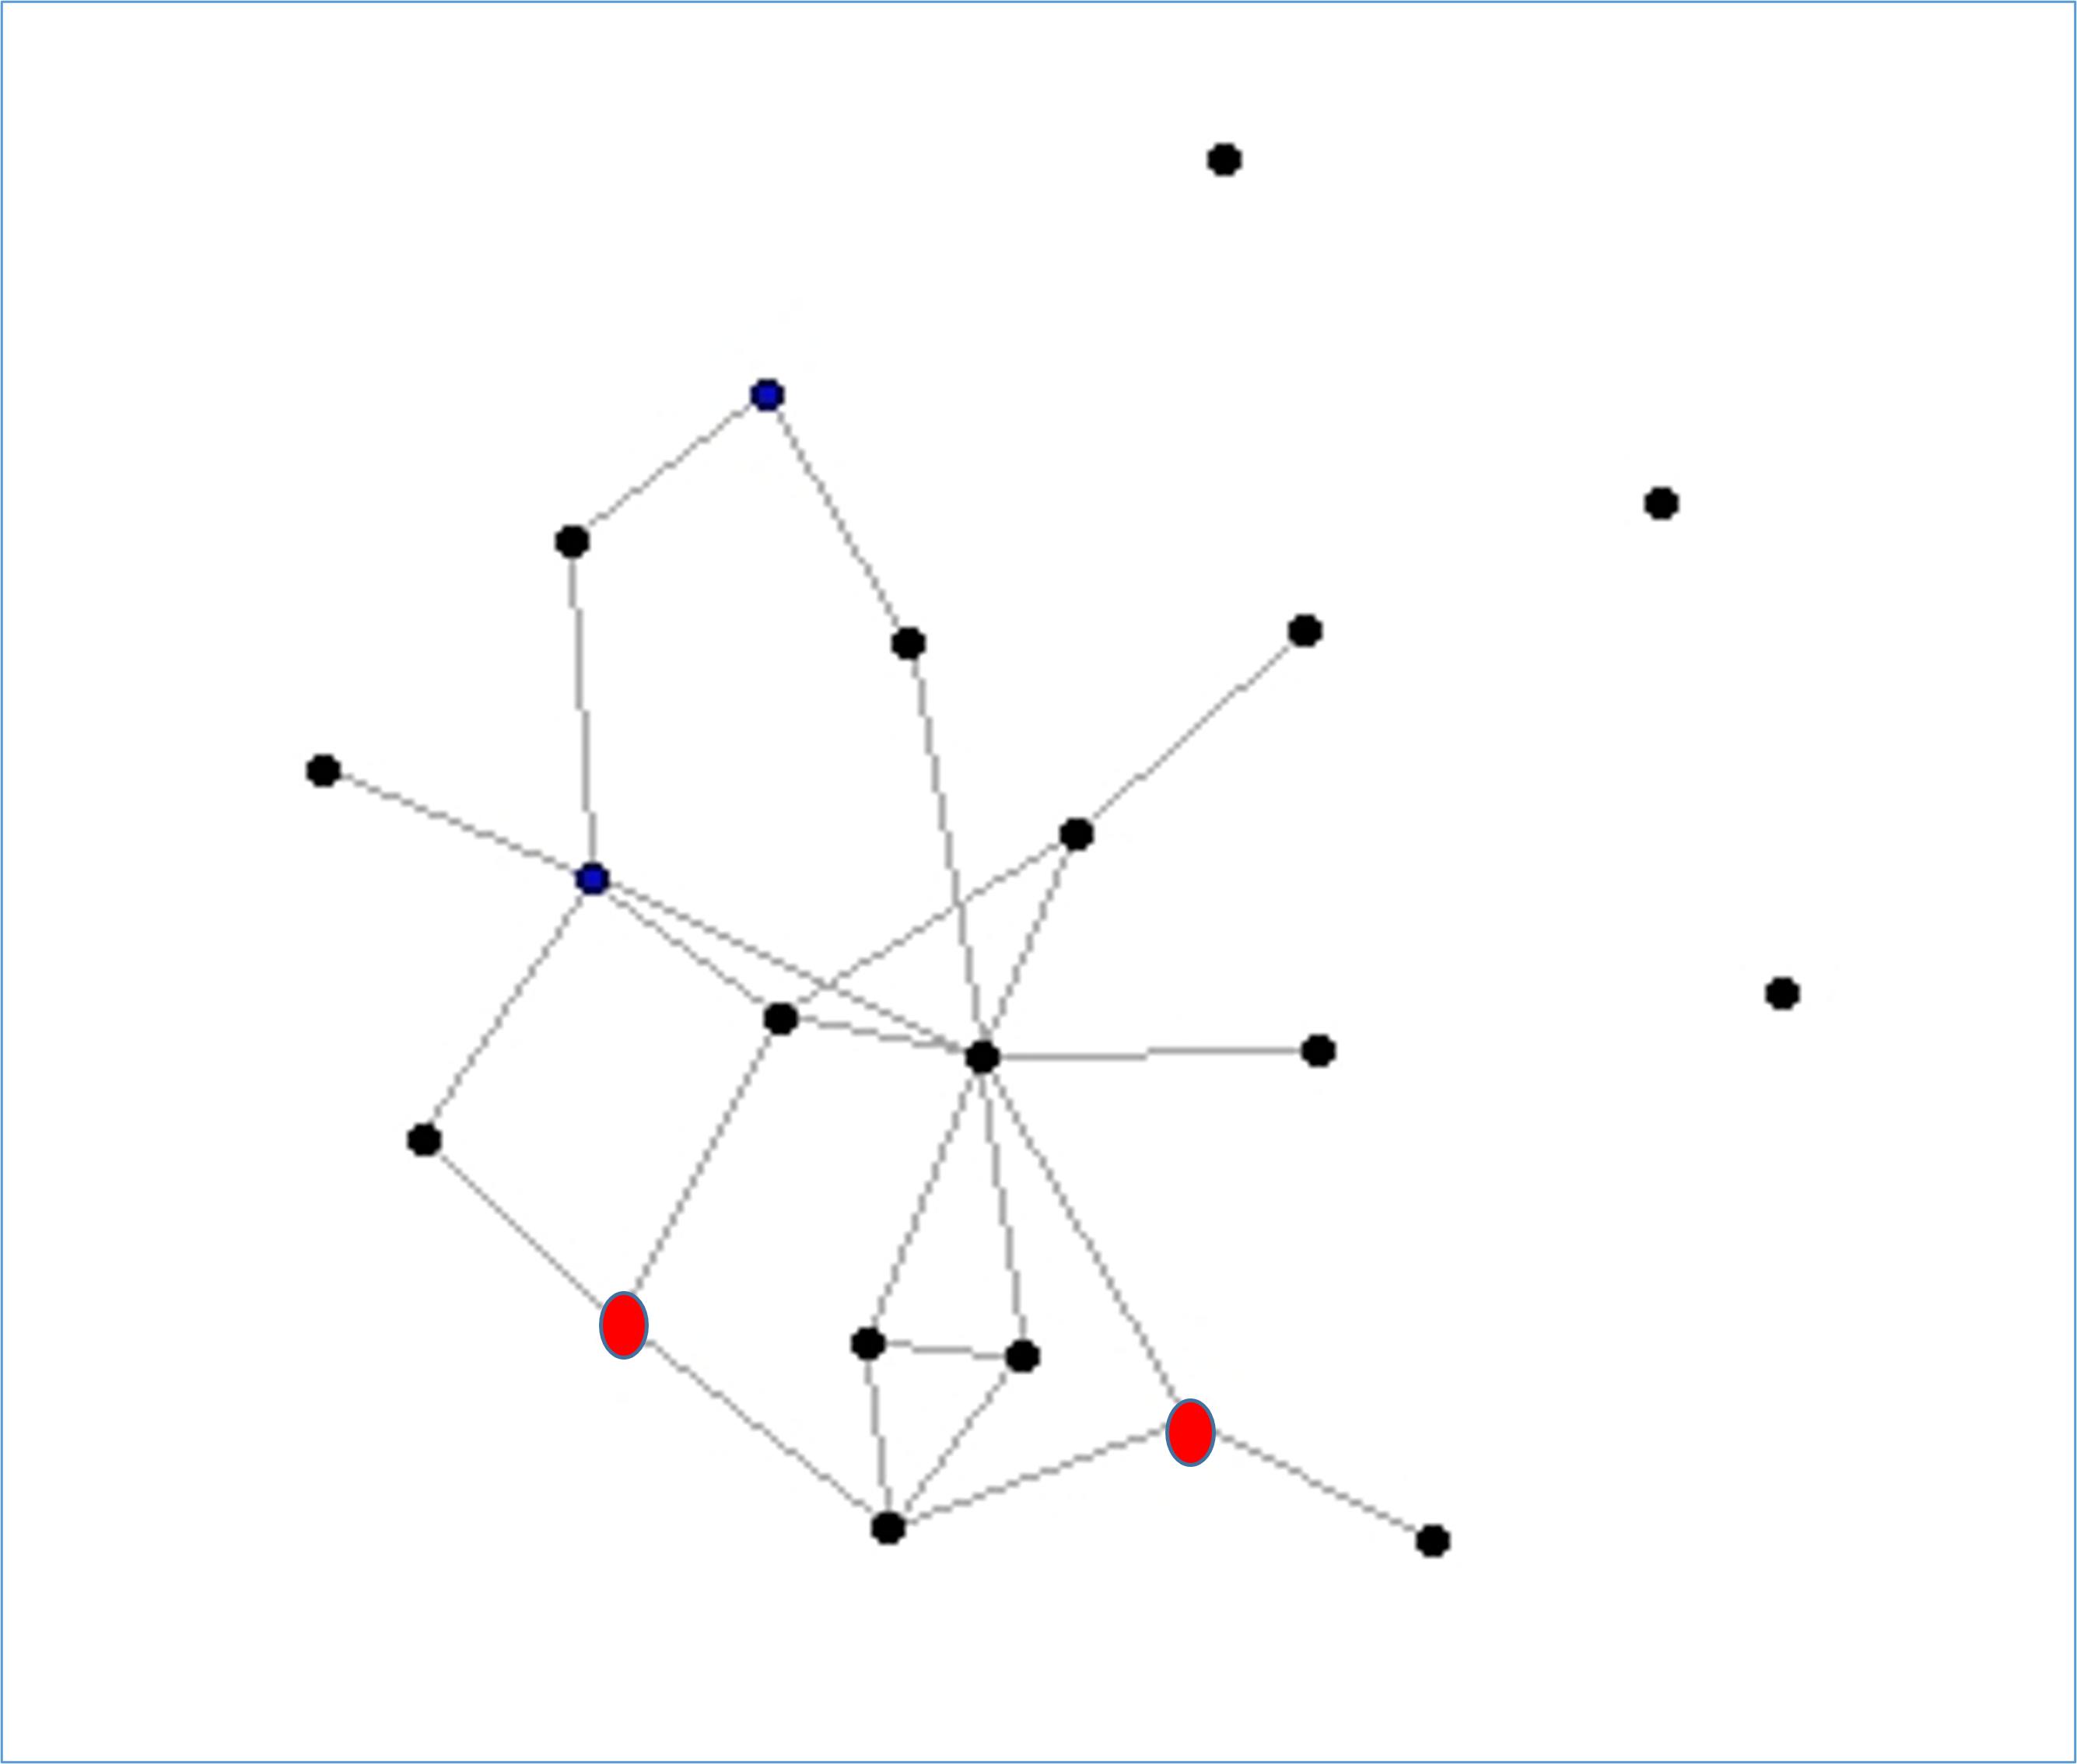
\includegraphics[scale=0.5]{Figures/Network Example 1.png}
    \caption{Control data generated for network example. 2 red nodes represent HIV positive individuals. 18 black nodes represent uninfected individuals.}
    \label{fig: Figure 2}
\end{figure}
Consider the control network in Figure \ref{fig: Figure 2}  above with 20 nodes and a probability of HIV infection of 10\%. If we want to estimate the Overall Effect of 20\% PrEP use vs. 10\% PrEP use, we assume: HIV status is known and PrEP not assigned to PHIV; PrEP is assigned to individuals without HIV at random; Single time-step iterations in the simulation to minimize interference.

 Of the 18 uninfected individuals (black nodes), 5 have an infectious contact. 13 individuals are uninfected with no infectious contacts.
\begin{figure}[H]
    \centering
    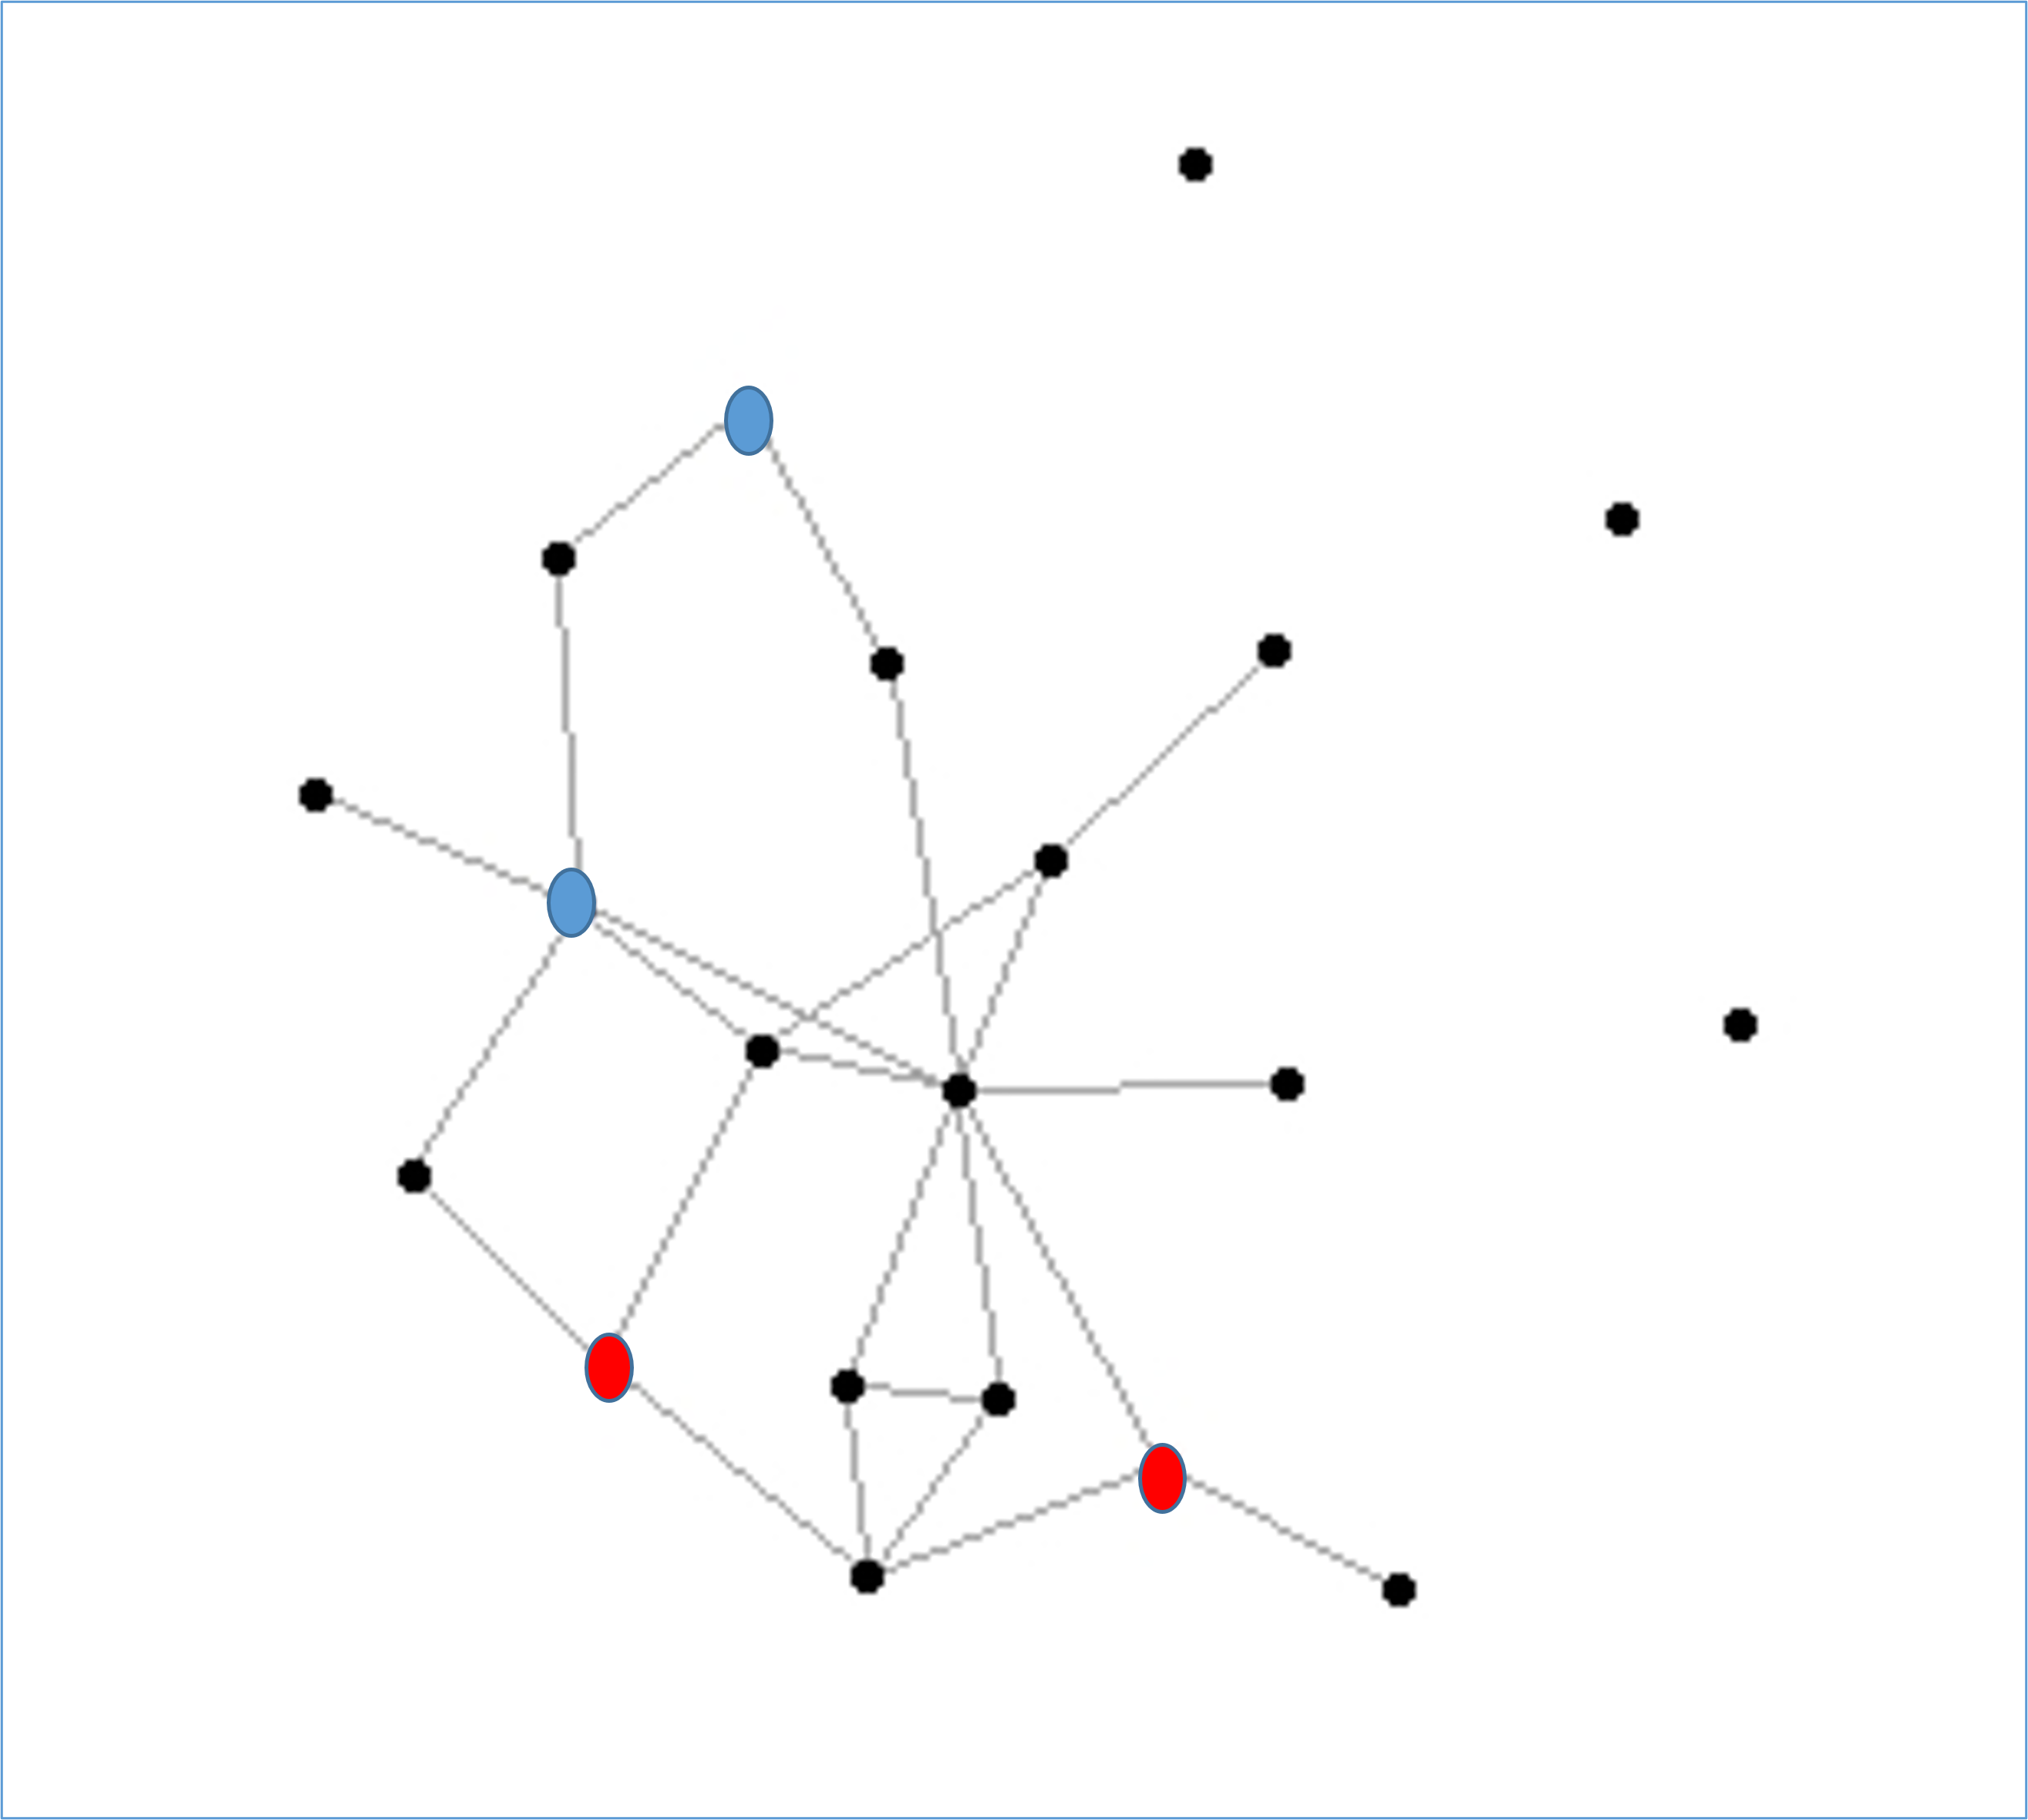
\includegraphics[scale=0.5]{Figures/Network Example 2.png}
    \caption{Random PrEP assignment to the network with 10\% coverage of uninfected individuals. 2 blue nodes represent uninfected individuals assigned to PrEP.}
    \label{fig:Figure 3}
\end{figure}

After PrEP assignment in Figure \ref{fig:Figure 3}. We can then compute probabilities of being infected given PrEP Assignment. Notice that neither of the 2 individuals assigned to PrEP are among the 5 uninfected individuals with known infectious contacts, so $$\mathbb{P}\left(\text{HIV}\vert \text{PrEP}\right)=\left(\frac{2}{2}\right)0=0.$$
Likewise, there are 16 uninfected individuals who were not assigned to PrEP, of whom 5 have an infectious contact. Let $p_{1}=\mathbb{P}\left(\text{HIV} \vert \text{infectious contact} \cap \neg \text{PrEP}\right)$ denote the probability of HIV infection given at least one infectious contact and not being assigned to PrEP.  Then, $$\mathbb{P}\left(\text{HIV} \vert \text{PrEP}^c\right)=\frac{5}{16}p_{1}+\left(\frac{11}{16}\right)0=\frac{5}{16}p_{1}.$$ Note, there is no HIV risk for those without infectious contacts.
\subsection{Treatment Scenario 1} 
\begin{figure}[H]
    \centering
    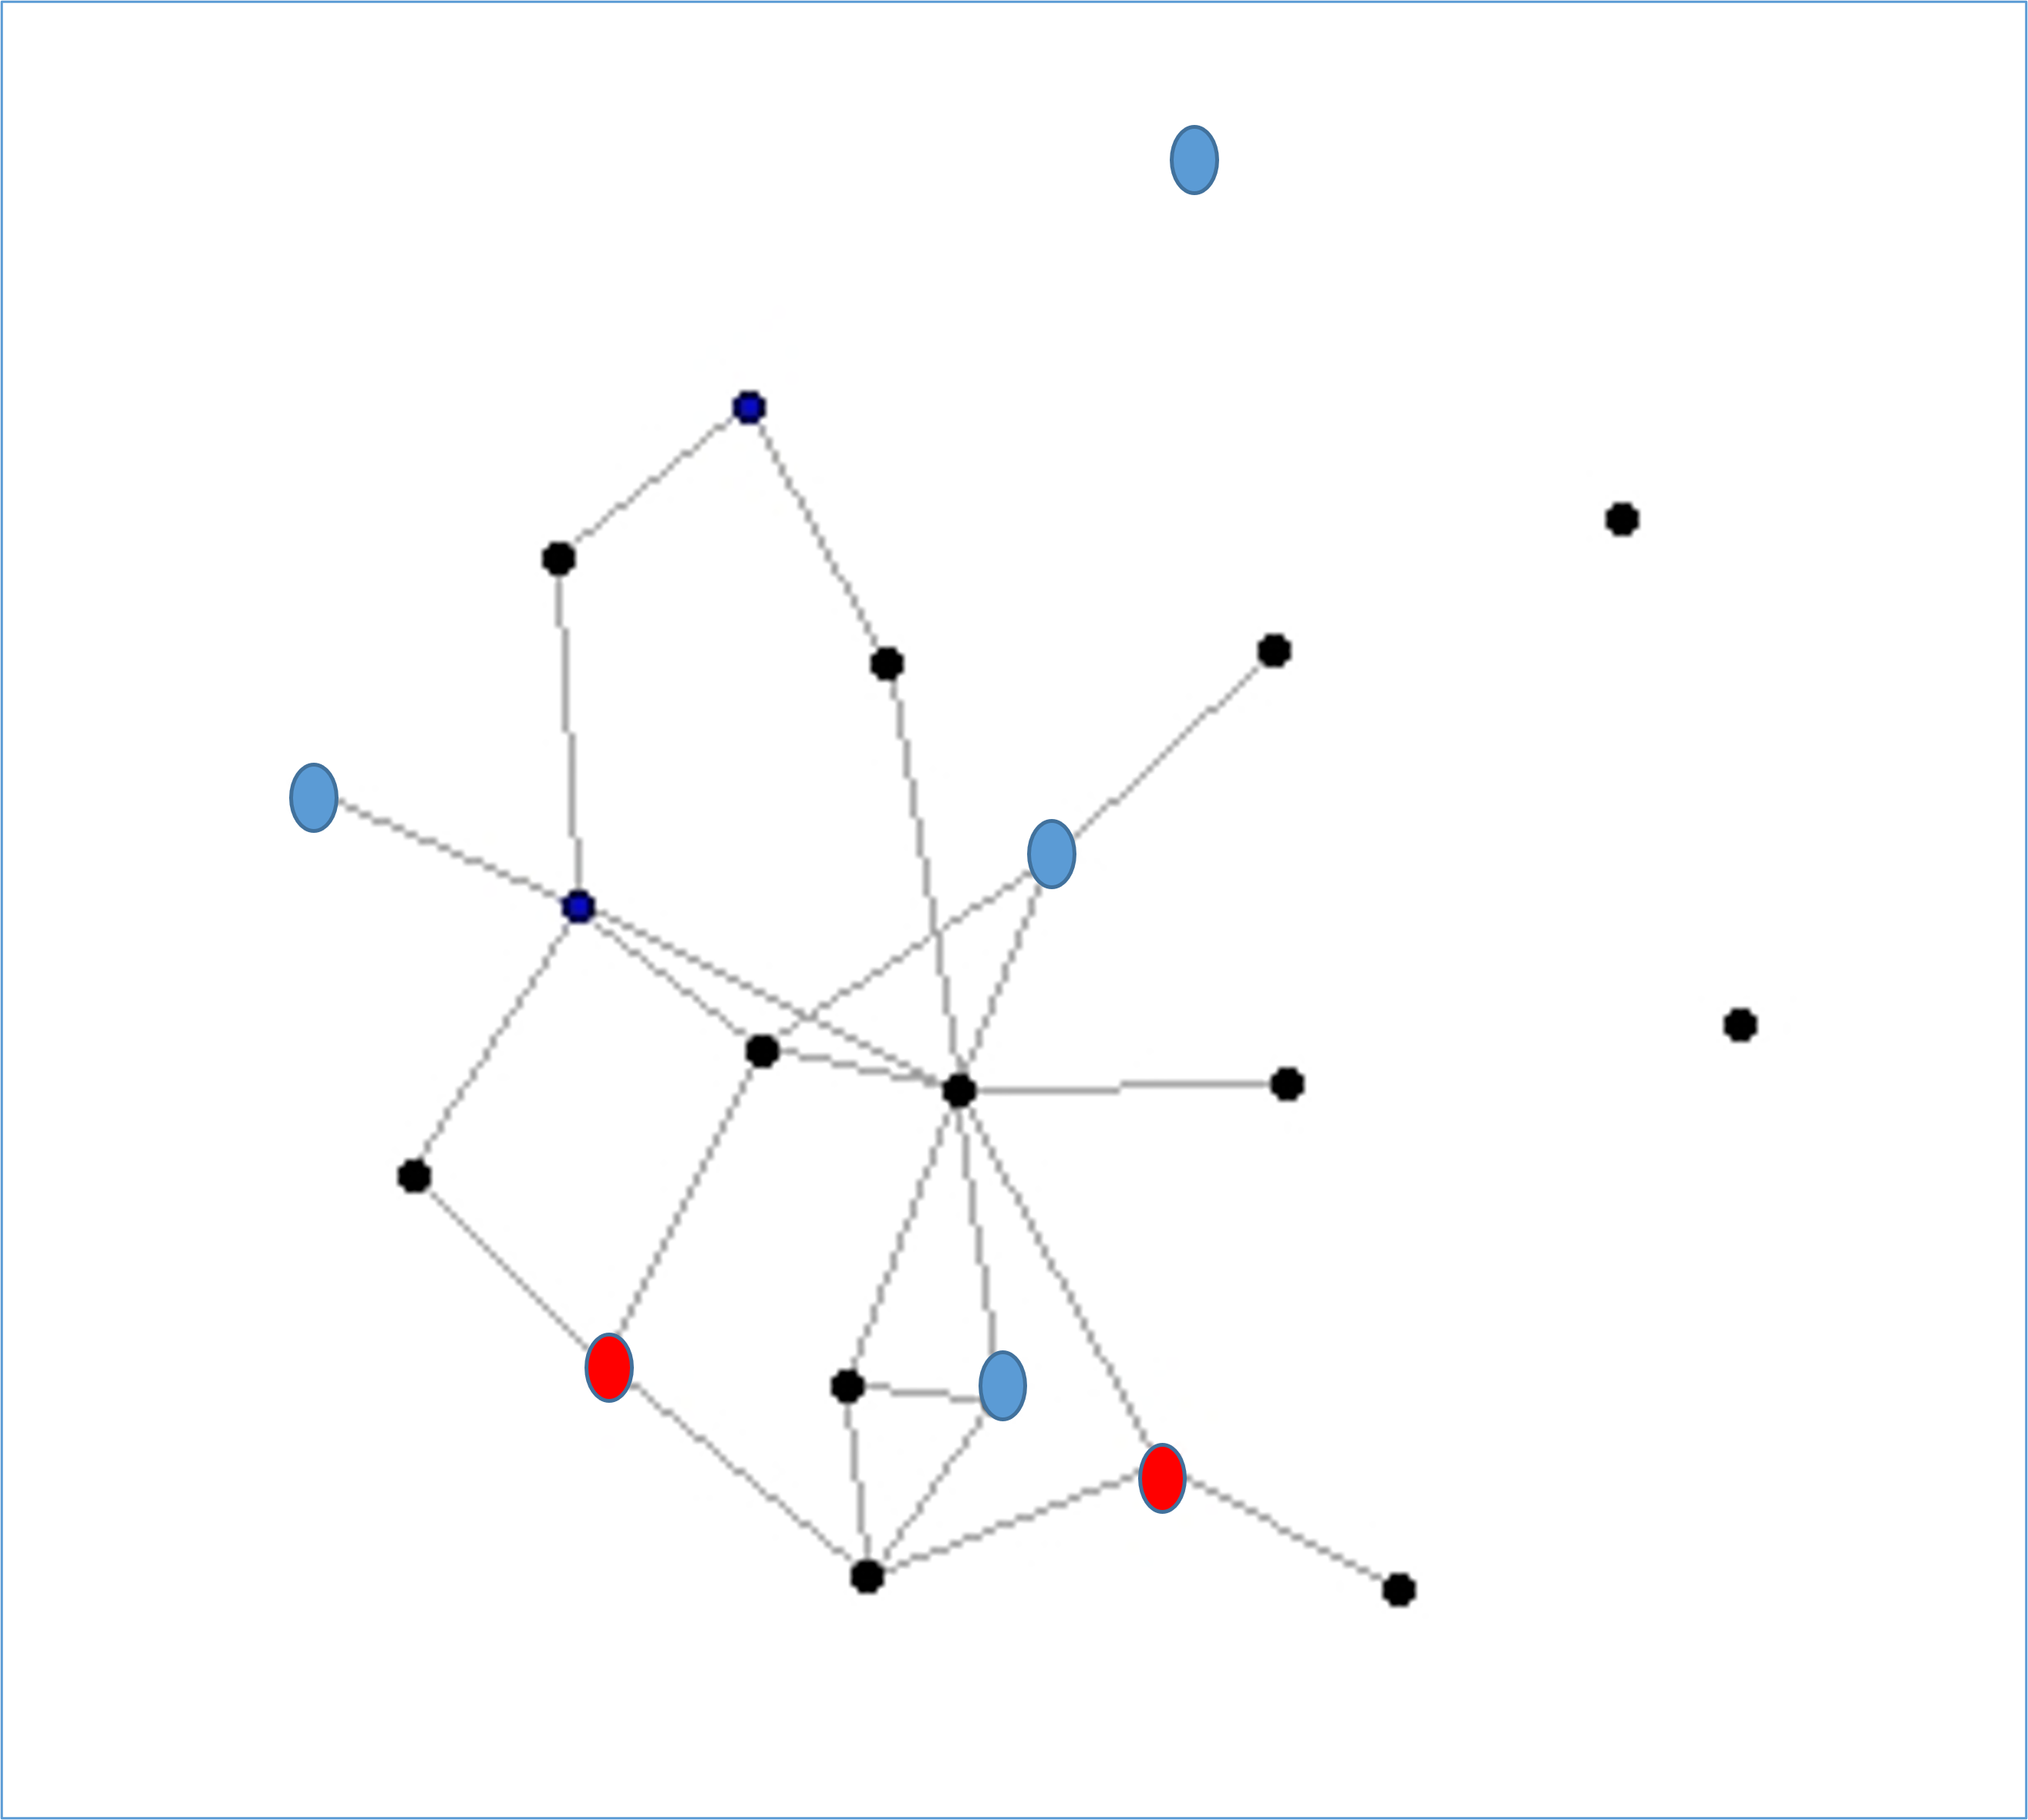
\includegraphics[scale=0.5]{Figures/Network Example 3.png}
    \caption{Treatment Option 1: Randomly assigned 20 \% coverage (blue nodes) to the uninfected individuals.}
    \label{fig:Figure 4}
\end{figure}

One option is to randomly assign 20 \% PrEP coverage to uninfected individuals, as in Figure \ref{fig:Figure 4} above.
We can see that 4 uninfected individuals were assigned to PrEP, but none of these have an infectious contact. So, $$\mathbb{P}\left[\text{HIV}\vert \text{PrEP} \right]=0.$$ Likewise, there are 14 uninfected individuals in the network who have been assigned no PrEP, 5 of whom have an infectious contact. Thus, $$\mathbb{P}\left[\text{HIV} \vert \neg \text{ PrEP}\right]=\frac{5}{14}p_{1}+\frac{9}{14}\left(0\right).$$  

\subsection{Treatment Scenario 2} 
\begin{figure}[H]
    \centering
    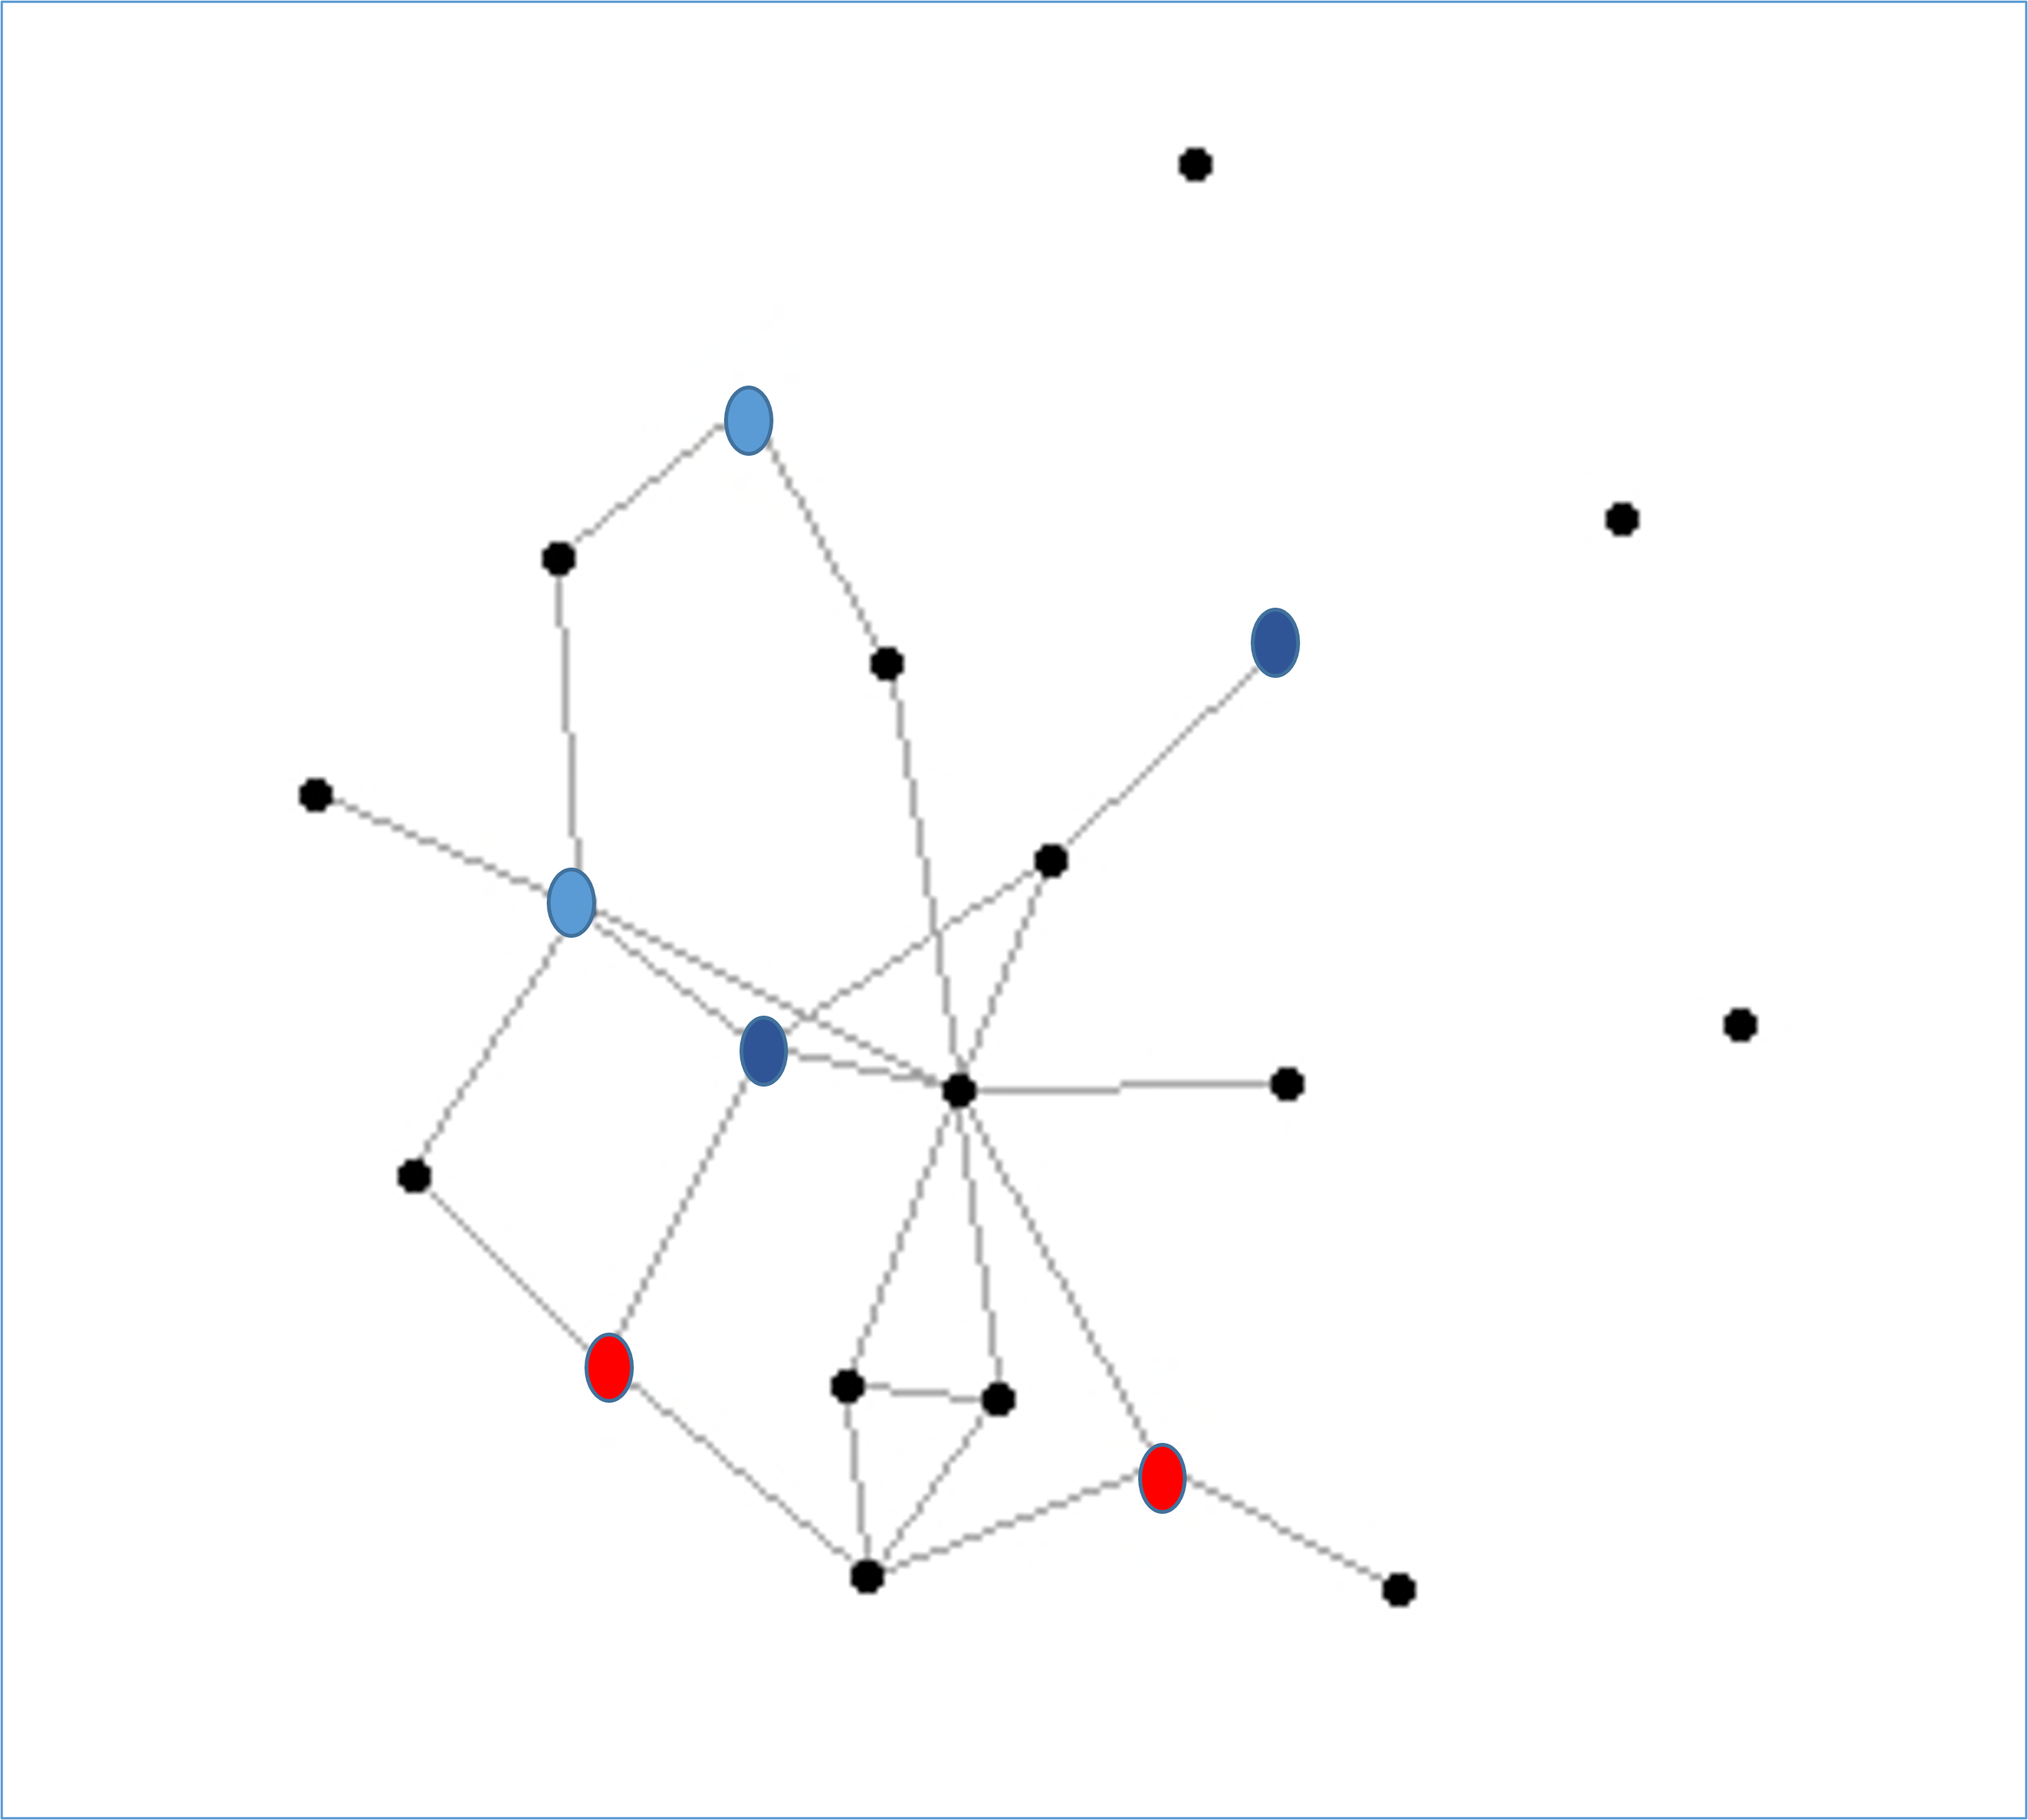
\includegraphics[scale=0.5]{Figures/Network Example 4.png}
    \caption{Treatment Option 2: Randomly assign an additional 10\% PrEP coverage to the Control Scenario network for a total coverage of 20\%. 2 uninfected individuals from the control scenario (light blue nodes) were assigned PrEP. 2 additional uninfected individuals (dark blue nodes) were assigned PrEP. }
    \label{fig:Figure 5}
\end{figure}

Another option is to assign PrEP coverage to an additional 10 \% remaining uninfected individuals from the control scenario. See Figure \ref{fig:Figure 5} above. 
We can see that 2 uninfected individuals have been assigned to PrEP, neither of whom have an infectious contact. 2 additional uninfected individuals were assigned PrEP, one of whom has an infectious contact. Let $p_{2}=\mathbb{P}\left[\text{HIV } \vert \text{ infectious contact} \cap \text{PrEP}\right].$ Then, $$\mathbb{P}\left[\text{HIV } \vert \text{ PrEP}\right]=\frac{1}{4}p_{2}+\frac{3}{4}\left(0\right).$$  
14 uninfected individuals have been assigned no PrEP, 5 of whom have an infectious contact. So, $$\mathbb{P}\left[\text{HIV } \vert \neg \text{ PrEP}\right]=\frac{5}{14}p_{1}+\frac{9}{14}\left(0\right).$$
\subsection{Treatment Scenario 3}
\begin{figure}[H]
    \centering
    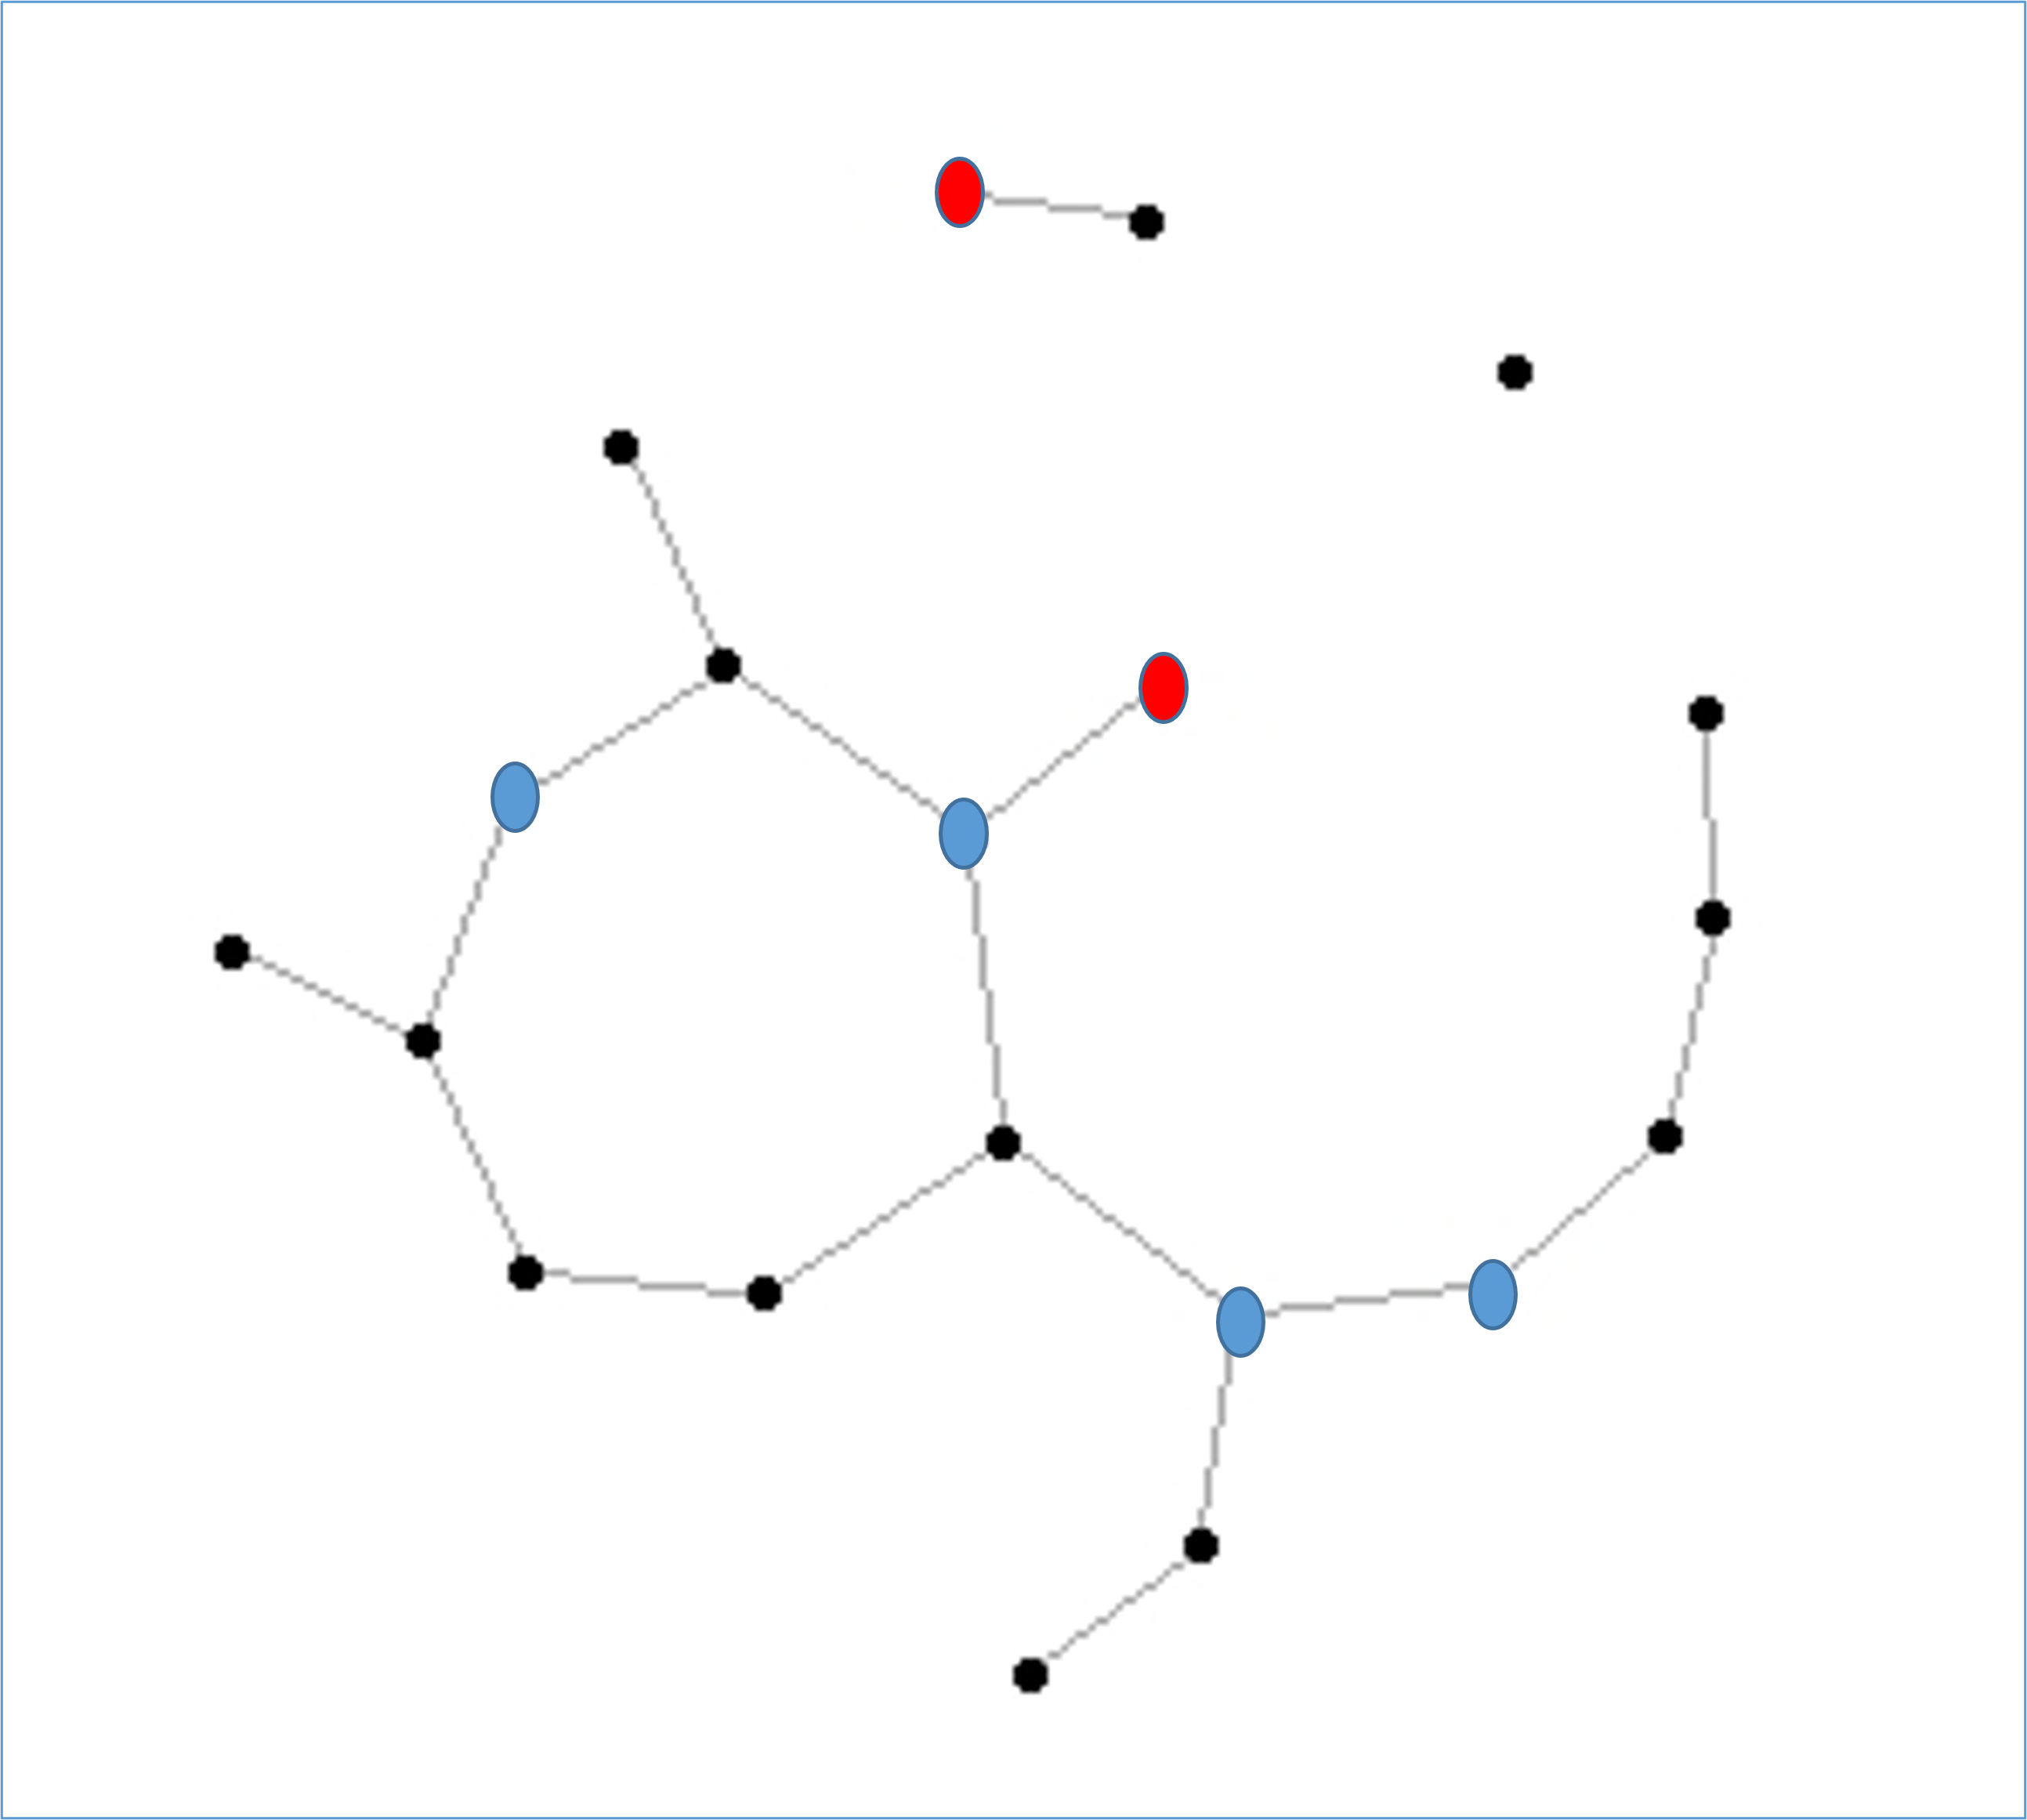
\includegraphics[scale=0.5]{Figures/Network Example 5.png}
    \caption{Treatment Option 3: Re-generate the network and randomly assign 20 \% PrEP coverage. 2 individuals are infected (red nodes). There are 4 uninfected individuals assigned to PrEP (light blue nodes), of whom one has an infectious contact. }
    \label{fig:Figure 6}
\end{figure}

Yet another option is to regenerate the network and randomly assign 20 \% PrEP coverage. See Figure \ref{fig:Figure 6} above. There are 2 infected individuals and 18 uninfected individuals. 2 uninfected individuals have infectious contacts. 4 uninfected individuals have been assigned to PrEP, one of whom has an infectious contact. Thus, $$\mathbb{P}\left[\text{HIV } \vert \text{PrEP}\right]=\frac{1}{4}p_{2}+\frac{3}{4}\left(0\right).$$
There are 14 uninfected individuals who have been assigned no PrEP, one of whom has an infectious contact. Hence, $$\mathbb{P}\left[\text{HIV } \vert \neg \text{ PrEP}\right]=\frac{1}{14}p_{1}+\frac{13}{14}\left(0\right).$$
\subsection{Effect Estimates}
We can now compute and compare the effect of 20\% PrEP coverage vs. 10\% PrEP coverage for each of the 3 scenarios.
\begin{center}
    \begin{tabular}{|c|c|c|}
    \hline
    PrEP Assignment Scenario     & $\mathbb{P}\left[\text{HIV} \vert \text{PrEP}\right]$ &  Effect Estimate  \\
         \hline
      10 \% Control   & $\frac{5}{18}p_{1}$ & NA\\
      \hline
      20\% random assignment on control network & $\frac{5}{18}p_{1}$ & 0 \\
      \hline
      20 \% from random additional 10\% on control network & $\frac{1}{18}p_{2}+\frac{5}{18}p_{1}$ & $\frac{1}{18}p_{2}$\\
      \hline
      20 \% random assignment on regenerated network & $\frac{1}{18}\left[p_{1}+p_{2}\right]$ & $\frac{1}{18}p_{2}-\frac{4}{18}p_{1}$\\
      \hline                 
    \end{tabular}                                      
    \end{center}
\section{Methods}
\subsection{Network Models}
Let $G=(V,E)$ be a graph representation of a network, with vertex set $V$ and edge set $E$. Let $N$ denote the \textit{order} of $G$, equal to the cardinality of the vertex set $\vert V \vert$. Network models are parameterized according to network size (graph order), and the generative model specifying the probability distribution from which the graph is drawn or the algorithm used to construct the graph. Let $deg(v)$ denote the degree of node $v$.

The simplest model considered is the  Erdős–Rényi (ER) Random Graph Model, with the $G(N,p)$ parameterization. This has the degree distribution function where each of $N$ nodes has a binomially-distributed degree:
\begin{equation*}
    \mathbb{P}(deg(v)=k)=\binom{n-1}{k}p^{k}\left(1-p\right)^{n-1-k}, \quad \forall v \in V . 
\end{equation*}

Two other network generative models were considered to incorporate specific aspects of network structure , namely \textit{preferential attachment} and \textit{clustering}. 

Preferential attachment is incorporated via the Barabási–Albert (BA) scale-free graph model. This model involves constructing an initial connected graph, then adding a new node at each time step which is connected to the existing node $i$ with probability 
\begin{equation*}
    p_{i}=\frac{k_{i}}{\sum_{j}k_{j}}.
\end{equation*}

This standard BA model has degree distribution
\begin{equation*}
    \mathbb{P}(deg(v)=k)=k^{-3}.
\end{equation*}
Note that we use a generalization of the Barabási–Albert model, sometimes called the Nonlinear Preferential Attachment Model with power parameter $\alpha$, where this probability is given by:
\begin{equation*}
    p_{i}=\frac{k_{i}^{\alpha}}{\sum_{j}k_{j}^{\alpha}}.
\end{equation*}

For notation convenience the NLPA model is still referred to as the BA model in this text.

To incorporate clustering, we used the Watts-Strogatz (WS) small world network model. The construction algorithm used here is different from the standard parameterization, and takes 4 parameters: the dimension of the initial lattice (here always equal to 1), the size of the graph in each dimension (here always the final graph order $N$), the connected \textit{neighborhood size} $n$, and the rewiring probability $r$. The initial graph is a lattice where each node is connected to its $n$ neighbors. From the initial lattice graph, edges are randomly ``rewired", i.e. removed and connected to a different node, uniformly with probability $r$.



Simulations were implemented in R 4.2.1. All code, data and figure files are available in the GitHub repository: \href{https://github.com/nico-dangelo/Network-Spillover}{Network Spillover}\footnote{https://github.com/nico-dangelo/Network-Spillover}. Network graphs were generated using igraph version 1.3.2.
\subsection{Static Simulations}

The Overall Effect (OE) was estimated according to the following:
%\begin{algorithm}
%   \SetKwInOut{KwIn}{Input}
%   \SetKwInOut{KwOut}{Output}
%   \KwIn{A vector of parameters (see above)}
%   \KwOut{A vector of contrast estimates [``random",``additive", ``regenerated"]}
%\end{algorithm}
    \begin{enumerate}
\item In each simulation iteration, let $G_{\text{control}}=\left(V_{\text{control}},E_{\text{control}}\right)$ be the ``control" network graph, with $\vert V_{\text{control}}\vert \eqqcolon N_{\text{control}}$. The vertex attributes of $V_{\text{control}}$ are initialized to one of three states: 
\begin{itemize}
        \item  $N_{HIV}(V_{\text{control}})=N_{\text{control}}p_{hiv}$ nodes are initialized to the  ``infectious" state.
        \item $N_{PrEP_{1}}\left(V_{\text{control}}\right)=\left[N_{\text{control}}-N_{HIV}\left(V_{\text{control}}\right)\right]p_{PrEP_{1}}$ nodes are initialized to the ``treated,susceptible" state. 
        \item The remaining $N_{\text{control}}-\left[N_{HIV}\left(V_{\text{control}}\right)+N_{PrEP_{1}}\left(V_{\text{control}}\right)\right]$ nodes are initialized to the ``untreated, susceptible" state.
    \end{itemize}
    \item The set $IC(V_{\text{control}})$ of susceptible nodes with at least one infectious contact is identified from each node's neighborhood.
    \item The probability of HIV given treatment in the control scenario, $\mathbb{P}(\text{HIV} \vert \text{PrEP})_{\text{control}}$ is computed:
    \begin{enumerate}
     
    \item We compute $\mathbb{P}\left( \text{PrEP} \cap \text{Infectious contact}\right)$ as the proportion of the treated set  $T(V_{\text{control}})$ that have an infectious contact: \begin{equation}
        \mathbb{P}\left( \text{PrEP} \cap \text{Infectious contact}\right)=\frac{\vert IC\left(V_{\text{control}}\right) \bigcap \left({T\left(V_{\text{control}}\right)}\right)\vert}{\vert T\left(V_{\text{control}}\right)\vert}.
    \end{equation}
    \item The probability $\mathbb{P}\left(\text{HIV} \vert \text{PrEP}\right)_{\text{control}}$ is then 
    \begin{equation}
        \mathbb{P}\left(\text{HIV} \vert \text{PrEP}\right)_{\text{control}}=\mathbb{P}\left(\text{HIV} \vert \text{PrEP} \cap \text{Infectious Contact}\right) \mathbb{P}\left(\text{PrEP} \cap \text{Infectious Contact}\right)
    \end{equation}
    \end{enumerate}
    \item We then similarly compute the probability of HIV given no treatment in the control scenario, $\mathbb{P} \left(\text{HIV} \vert \neg \text{PrEP}\right)_{\text{control}}$:
    \begin{enumerate}
    \item We compute $\mathbb{P}\left(\neg \text{PrEP} \cap \text{Infectious Contact} \right)  $ as the proportion of untreated susceptible nodes that have an infectious contact:
    \begin{equation}
        \mathbb{P}\left(\neg \text{PrEP} \cap \text{Infectious Contact} \right)=\frac{\vert IC\left(V_{\text{control}}\right) \bigcap \left({T'\left(V_{\text{control}}\right)}\right)\vert}{\vert T'\left(V_{\text{control}}\right)\vert},
    \end{equation}

    where $T'\left(V_{\text{control}}\right)$ denotes the set of untreated susceptible nodes.
    \item The probability $\mathbb{P}\left(\text{HIV} \vert \neg \text{PrEP}\right)_{\text{control}}$ is then
    \begin{equation}
        \mathbb{P}\left(\text{HIV} \vert \neg \text{PrEP}\right)_{\text{control}}=\mathbb{P}\left(\text{HIV} \vert \neg \text{PrEP} \cap \text{Infectious Contact}\right) \mathbb{P}\left( \neg \text{PrEP} \cap \text{Infectious Contact}\right).
    \end{equation}
    \end{enumerate}
    \item For the ``random" and ``additive" $\text{PrEP}_{2}$ treatment allocation  scenarios, the topology of $G_{\text{control}}$ is fixed, but treatment attributes on the vertex set are varied. 
    \begin{enumerate}
        \item For the ``random" $\text{PrEP}_{2}$ scenario, the infectious nodes from the control scenario are fixed, but the treatment set is instead a randomly selected $N_{\text{control}}PrEP_{2}$ nodes.
        %check me %
        \item For the ``additive" scenario, the infectious nodes are fixed, with the treated set $T\left(V_{\text{additive}}\right)$ contains the original treated nodes in addition to $\left[N_{\text{control}}-N_{HIV}-N_{PrEP1}\right]PrEP_{2}$ treated nodes.
    \end{enumerate}
    \item For the ``regenerated" treatment scenario, a new graph $G_{\text{regenerated}}=\left(V_{ \text{regenerated}},E_{\text{regenerated}}\right)$ with new attributes on the vertex set is generated.
    \begin{itemize}
        \item $N_{HIV}\left(V_{\text{regenerated}}\right)p_{hiv}$ nodes are assigned to the ``infectious" state.
        \item $N_{PrEP_{2}}\left(V_{\text{regenerated}}\right)=\left[N_{\text{regenerated}}\left(V_{\text{regenerated}}\right)-N_{HIV}\left(V_{\text{regenerated}}\right)\right]p_{PrEP_{2}}$ nodes are assigned to the ``susceptible, treated" state. 
    \end{itemize}
    \item The probabilities of infection with and without treatment are then computed similarly to the control scenario.
    \item The combined probability of HIV is computed, given each PrEP coverage and allocation
    \item The contrast estimate between each of the counterfactual allocations (``random", ``additive", ``regenerated") and the control are computed as the difference  between each of these combined probabilities and that for the control.
    \item These simulations are repeated $n_{sim}$ times and the means of these contrast estimates are computed.
\end{enumerate}
% \begin{table}[H]
%     \centering
%     \begin{tabular}{|c|c|c|}
%     \hline
%          \bf Object &  \bf Definition & \bf Variable name/alias in code  \\
%         \hline
%          $G_{\text{control}}=\left(V_{\text{control}},E_{\text{control}}\right)$& Network Graph for the control scenario & g \\
%      \hline
%      N_{\text{control}} & 
%     \end{tabul ar}
%     \caption{Notation for Static Simulation Effect Estimation}
%     \label{tab:my_label}
% \end{table}

%\subsection{Dynamic Simulations}

\section{Results}
\subsection{Erdős–Rényi  Random Graph Models}
We now display simulation results for various parameter combinations in the Erdős–Rényi Random Graph Model.
\begin{center}
    \begin{tabular}{|c|c|c|c|}
    \hline
         \bf Parameter & Alias in Code &  Default Value & Range Considered  \\
         \hline
         Network size & $N$& 20 & $\Set{20,50,200}$\\
         \hline
         ER Edge Formation probability & ``eprob" & 0.1 & Fixed \\
         \hline
         HIV prevalence & ``phiv" & 0.1 & $[0.1,0.8]$\\
         \hline
         Control PrEP Coverage &  ``PrEP1" & 0.2 & $[0.1,1]$\\
         \hline
         Counterfactual PrEP Coverage & ``PrEP2" & 0.4 & $[0.1,1]$\\
         \hline
         $\mathbb{P}\left[\text{HIV} \vert \neg \text{PrEP} \cap \text{Contact}\right]$ & $p1$ & 0.2 & $[0.1,1]$\\
         \hline
         $\mathbb{P}\left[\text{HIV} \vert \text{PrEP} \cap \text{Contact}\right]$ & $p2$  & 0.1 & $[0.1,1]$\\
         \hline
         Re-sampling sample size & ``nsim" & 200 & $\Set{100,1000,10000}$\\
         \hline
    \end{tabular}
\end{center}
\subsubsection{Effect Modification by Network Size}
\begin{figure}[H]
    \centering
    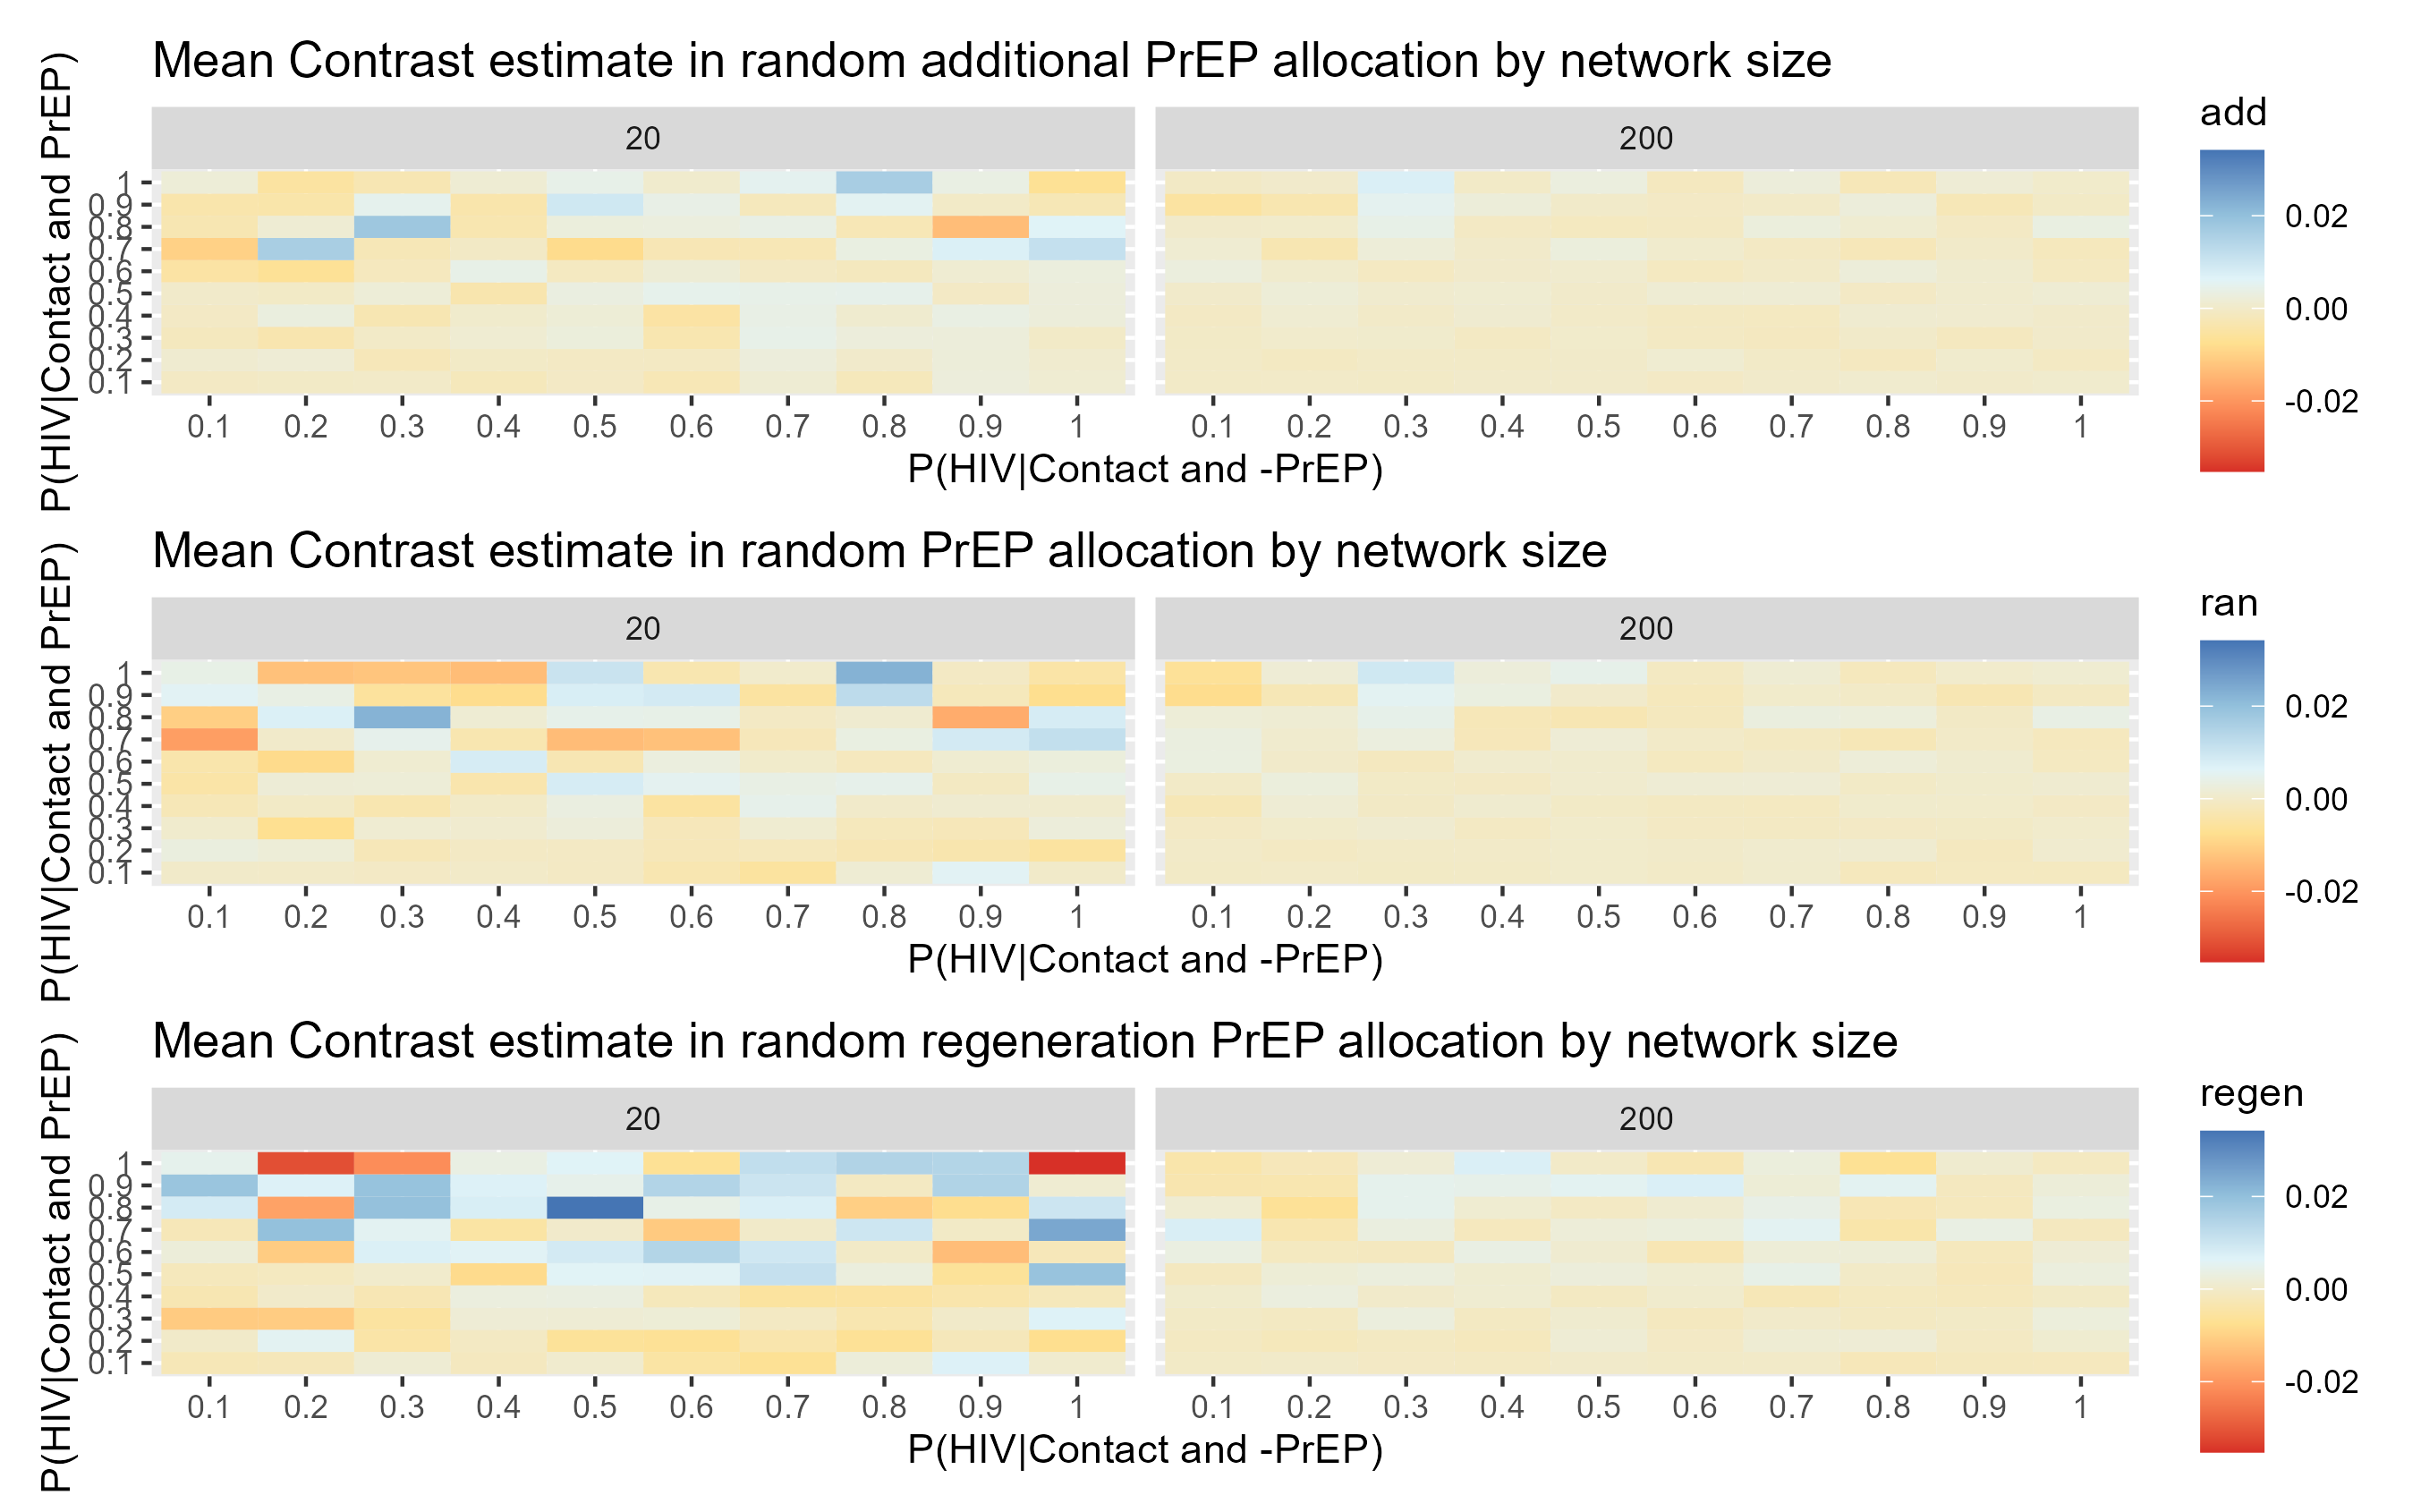
\includegraphics[width=\linewidth]{Figures/Network Size Mean Plot.png}
    \caption{Mean Causal Contrast estimates as $\mathbb{P}\left[\text{HIV} \vert \neg \text{PrEP} \cap \text{Contact}\right]$ and $\mathbb{P}\left[\text{HIV} \vert \text{PrEP} \cap \text{Contact}\right]$ increase, stratified by Network Size/Graph Order. From top to bottom: ``additive" Mean Contrast of random 20\% additional vs. random 20\% PrEP allocation control, ``random" Mean Contrast of random 40\% PrEP allocation vs. random 20\% control, ``regenerated" Mean Contrast of random 40\% allocation on regenerated network vs. random 20\% control. }
    \label{fig:Figure 7}
\end{figure}
\begin{figure}[H]
    \centering
    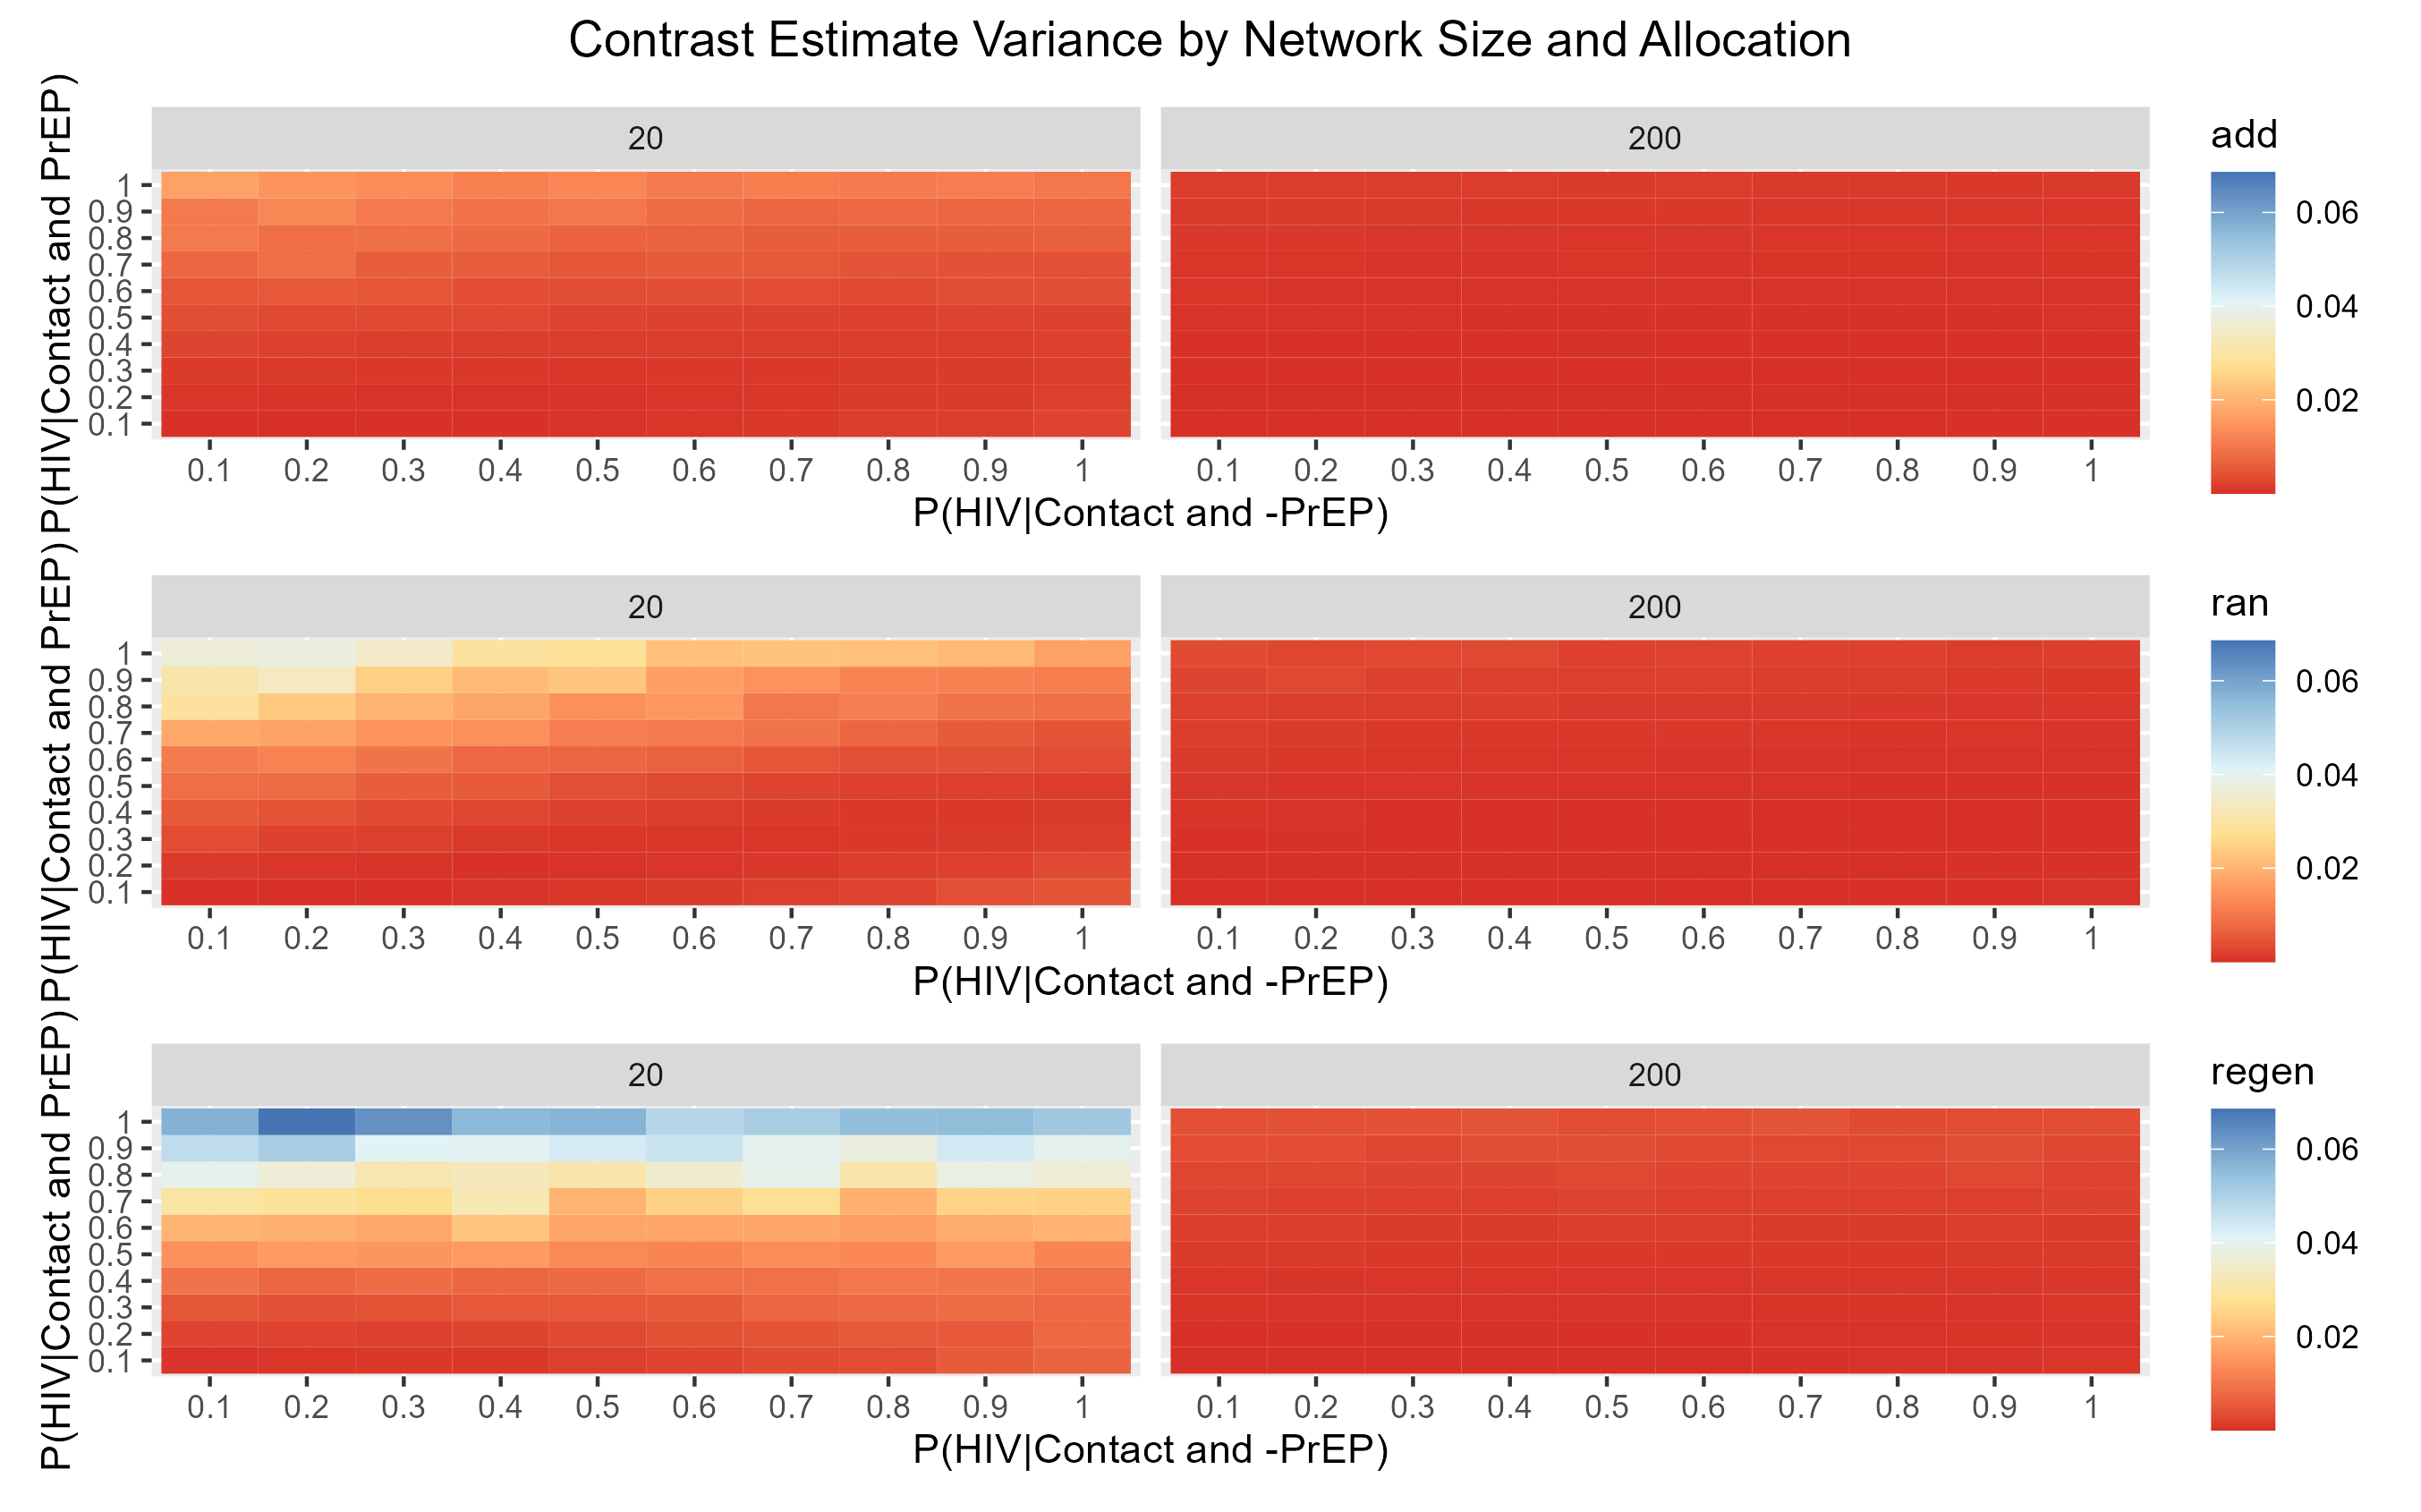
\includegraphics[width=\linewidth]{Figures/Network Size Variance plots.png}
    \caption{Variance of Causal Contrast estimates  as $\mathbb{P}\left[\text{HIV} \vert \neg \text{PrEP} \cap \text{Contact}\right]$ and $\mathbb{P}\left[\text{HIV} \vert \text{PrEP} \cap \text{Contact}\right]$ increase, stratified by Network Size/Graph Order. From top to bottom: ``additive" Variance of Contrast of random 20\% additional vs. random 20\% PrEP allocation control, ``random" Variance of Contrast of random 40\% PrEP allocation vs. random 20\% control, ``regenerated" Variance of Contrast of random 40\% allocation on regenerated network vs. random 20\% control.}
    \label{fig:Figure 8}
\end{figure}
From both the Mean and Variance plots above, there is apparent effect modification of the relationship between ``risks" of HIV and treatment allocation strategy at small network sizes. However, this modification essentially disappears in (order of magnitude) larger networks. The effect modification is particularly apparent with respect to the regenerated networks where the means are most variable across risk combinations (as well as the variances themselves).  

\subsubsection{Effect Modification by Sample Size}
\begin{figure}[H]
    \centering
    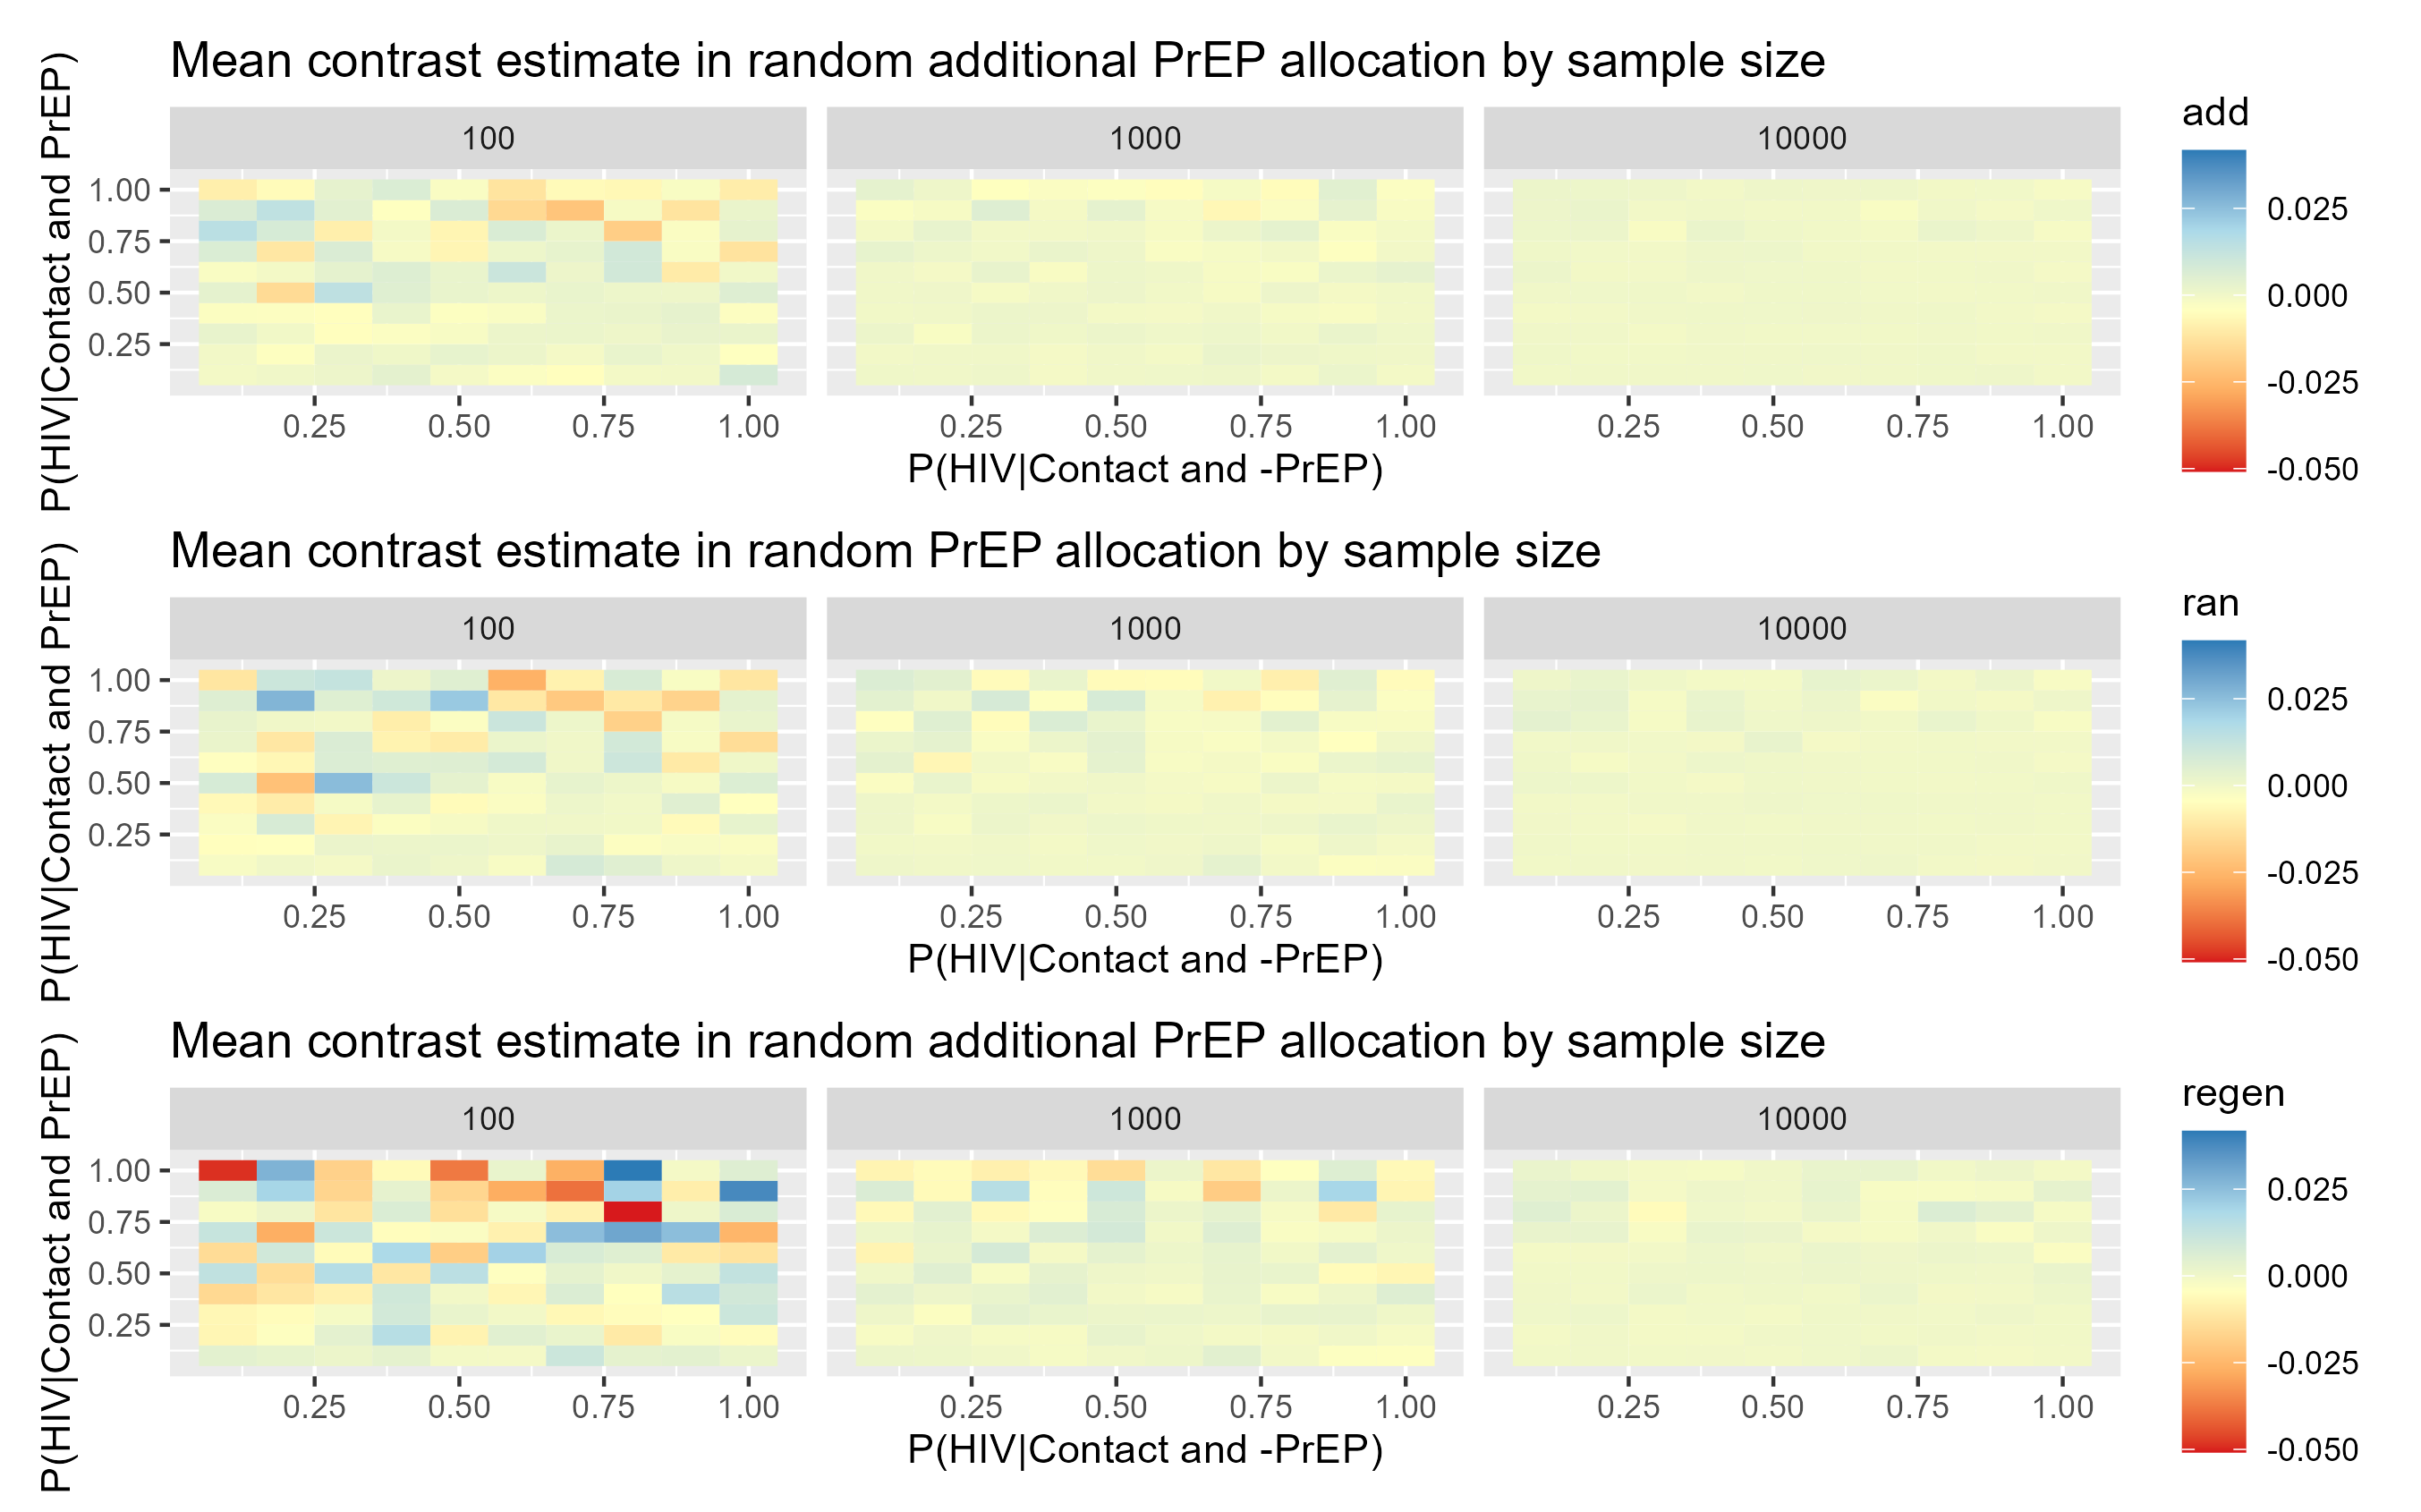
\includegraphics[width=\linewidth]{Figures/Sample size Mean plots.png}
    \caption{Mean Causal Contrast estimates as $\mathbb{P}\left[\text{HIV} \vert \neg \text{PrEP} \cap \text{Contact}\right]$ and $\mathbb{P}\left[\text{HIV} \vert \text{PrEP} \cap \text{Contact}\right]$ increase, stratified by resampling sample size. From top to bottom: ``additive" Mean Contrast of random 20\% additional vs. random 20\% PrEP allocation control, ``random" Mean Contrast of random 40\% PrEP allocation vs. random 20\% control, ``regenerated" Mean Contrast of random 40\% allocation on regenerated network vs. random 20\% control.}
    \label{fig:Figure 9}
\end{figure}
\begin{figure}[H]
    \centering
    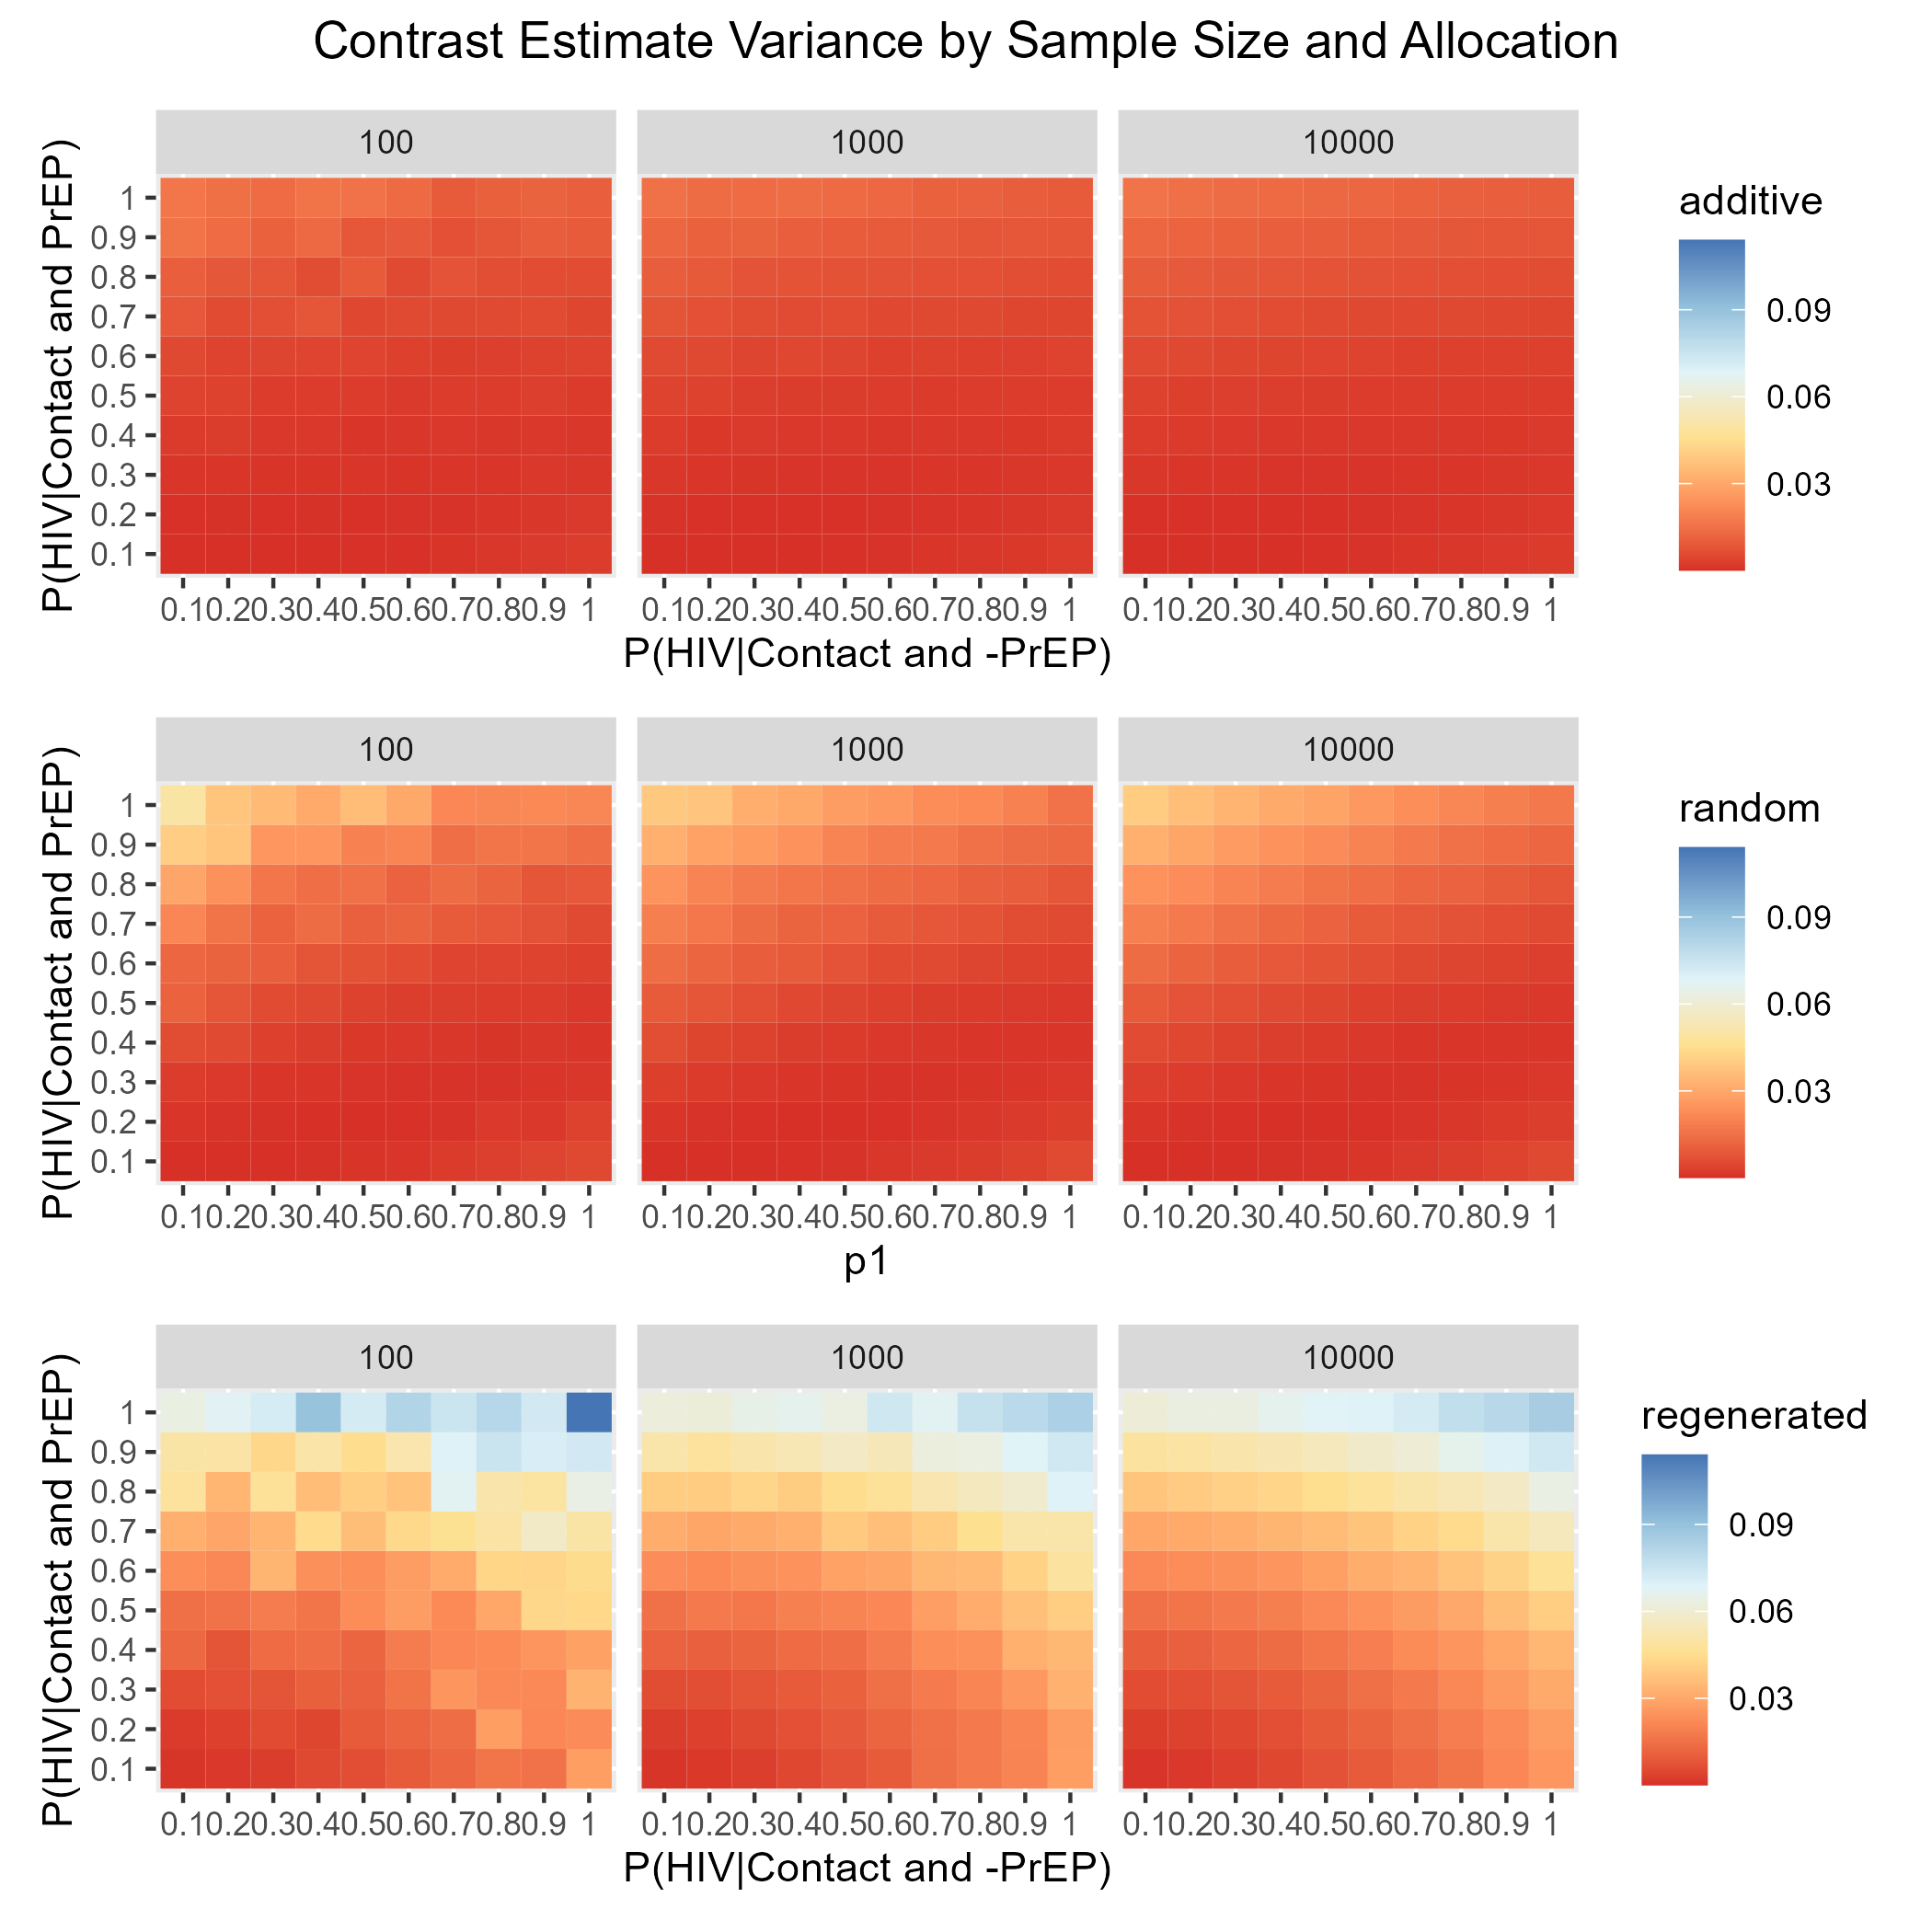
\includegraphics[width=\linewidth]{Figures/Sample Size Variance plots.png}
    \caption{Variance of Causal Contrast estimates as $\mathbb{P}\left[\text{HIV} \vert \neg \text{PrEP} \cap \text{Contact}\right]$ and $\mathbb{P}\left[\text{HIV} \vert \text{PrEP} \cap \text{Contact}\right]$ increase, stratified by resampling sample size. From top to bottom: ``additive" Variance of Contrast of random 20\% additional vs. random 20\% PrEP allocation control, ``random" Variance of Contrast of random 40\% PrEP allocation vs. random 20\% control, ``regenerated" Variance of Contrast of random 40\% allocation on regenerated network vs. random 20\% control.}
    \label{fig:Figure 10}
\end{figure}
Much like with network size, effect modification of the relationship between underlying HIV risks and treatment strategy by resampling size is apparent in both Mean and Variance plots above. We can see clearly from these plots that Contrast estimate variances differ not only in range of magnitudes, but also follow very different gradients under different treatment strategies.
\subsubsection{Effect Modification by HIV Prevalence}
\begin{figure}[H]
    \centering
    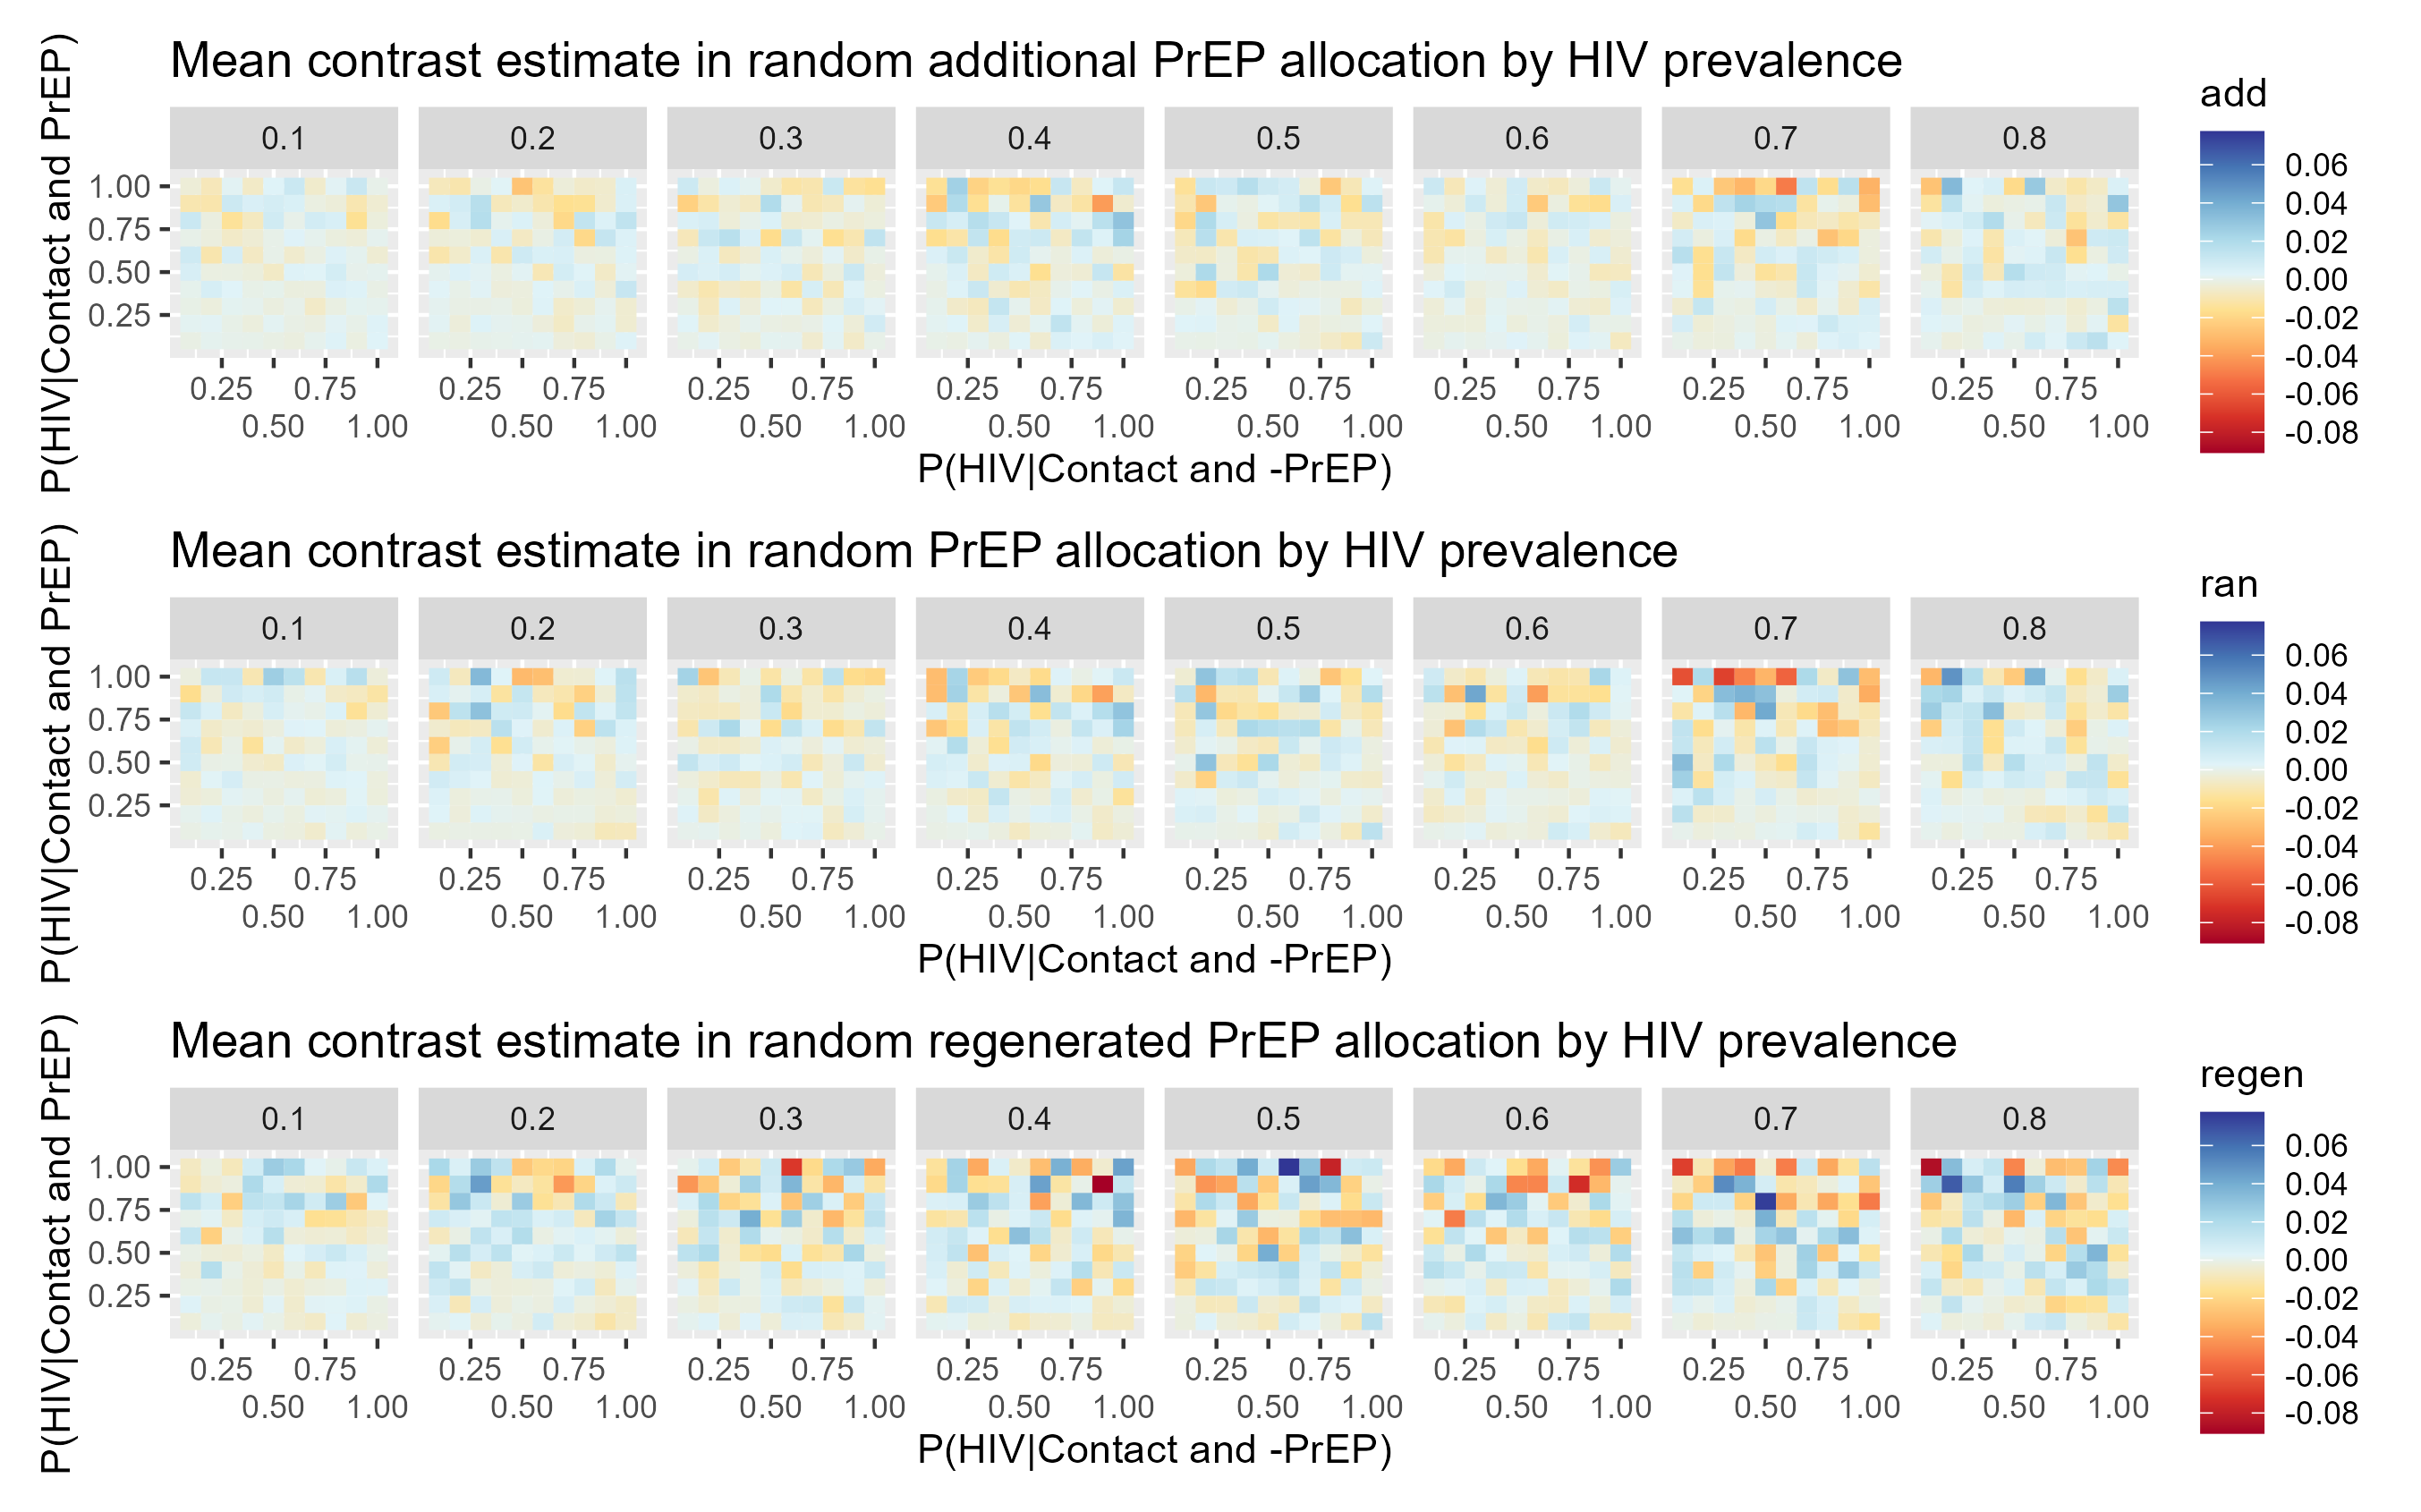
\includegraphics[width=\linewidth]{Figures/HIV Prevalence Mean plots.png}
    \caption{Mean Causal Contrast estimates as $\mathbb{P}\left[\text{HIV} \vert \neg \text{PrEP} \cap \text{Contact}\right]$ and $\mathbb{P}\left[\text{HIV} \vert \text{PrEP} \cap \text{Contact}\right]$ increase,  stratified by HIV Prevalence. From top to bottom: ``additive" Mean Contrast of random 20\% additional vs. random 20\% PrEP allocation control, ``random" Mean Contrast of random 40\% PrEP allocation vs. random 20\% control, ``regenerated" Mean Contrast of random 40\% allocation on regenerated network vs. random 20\% control.}
    \label{fig:Figure 11}
\end{figure}
\begin{figure}[H]
    \centering
    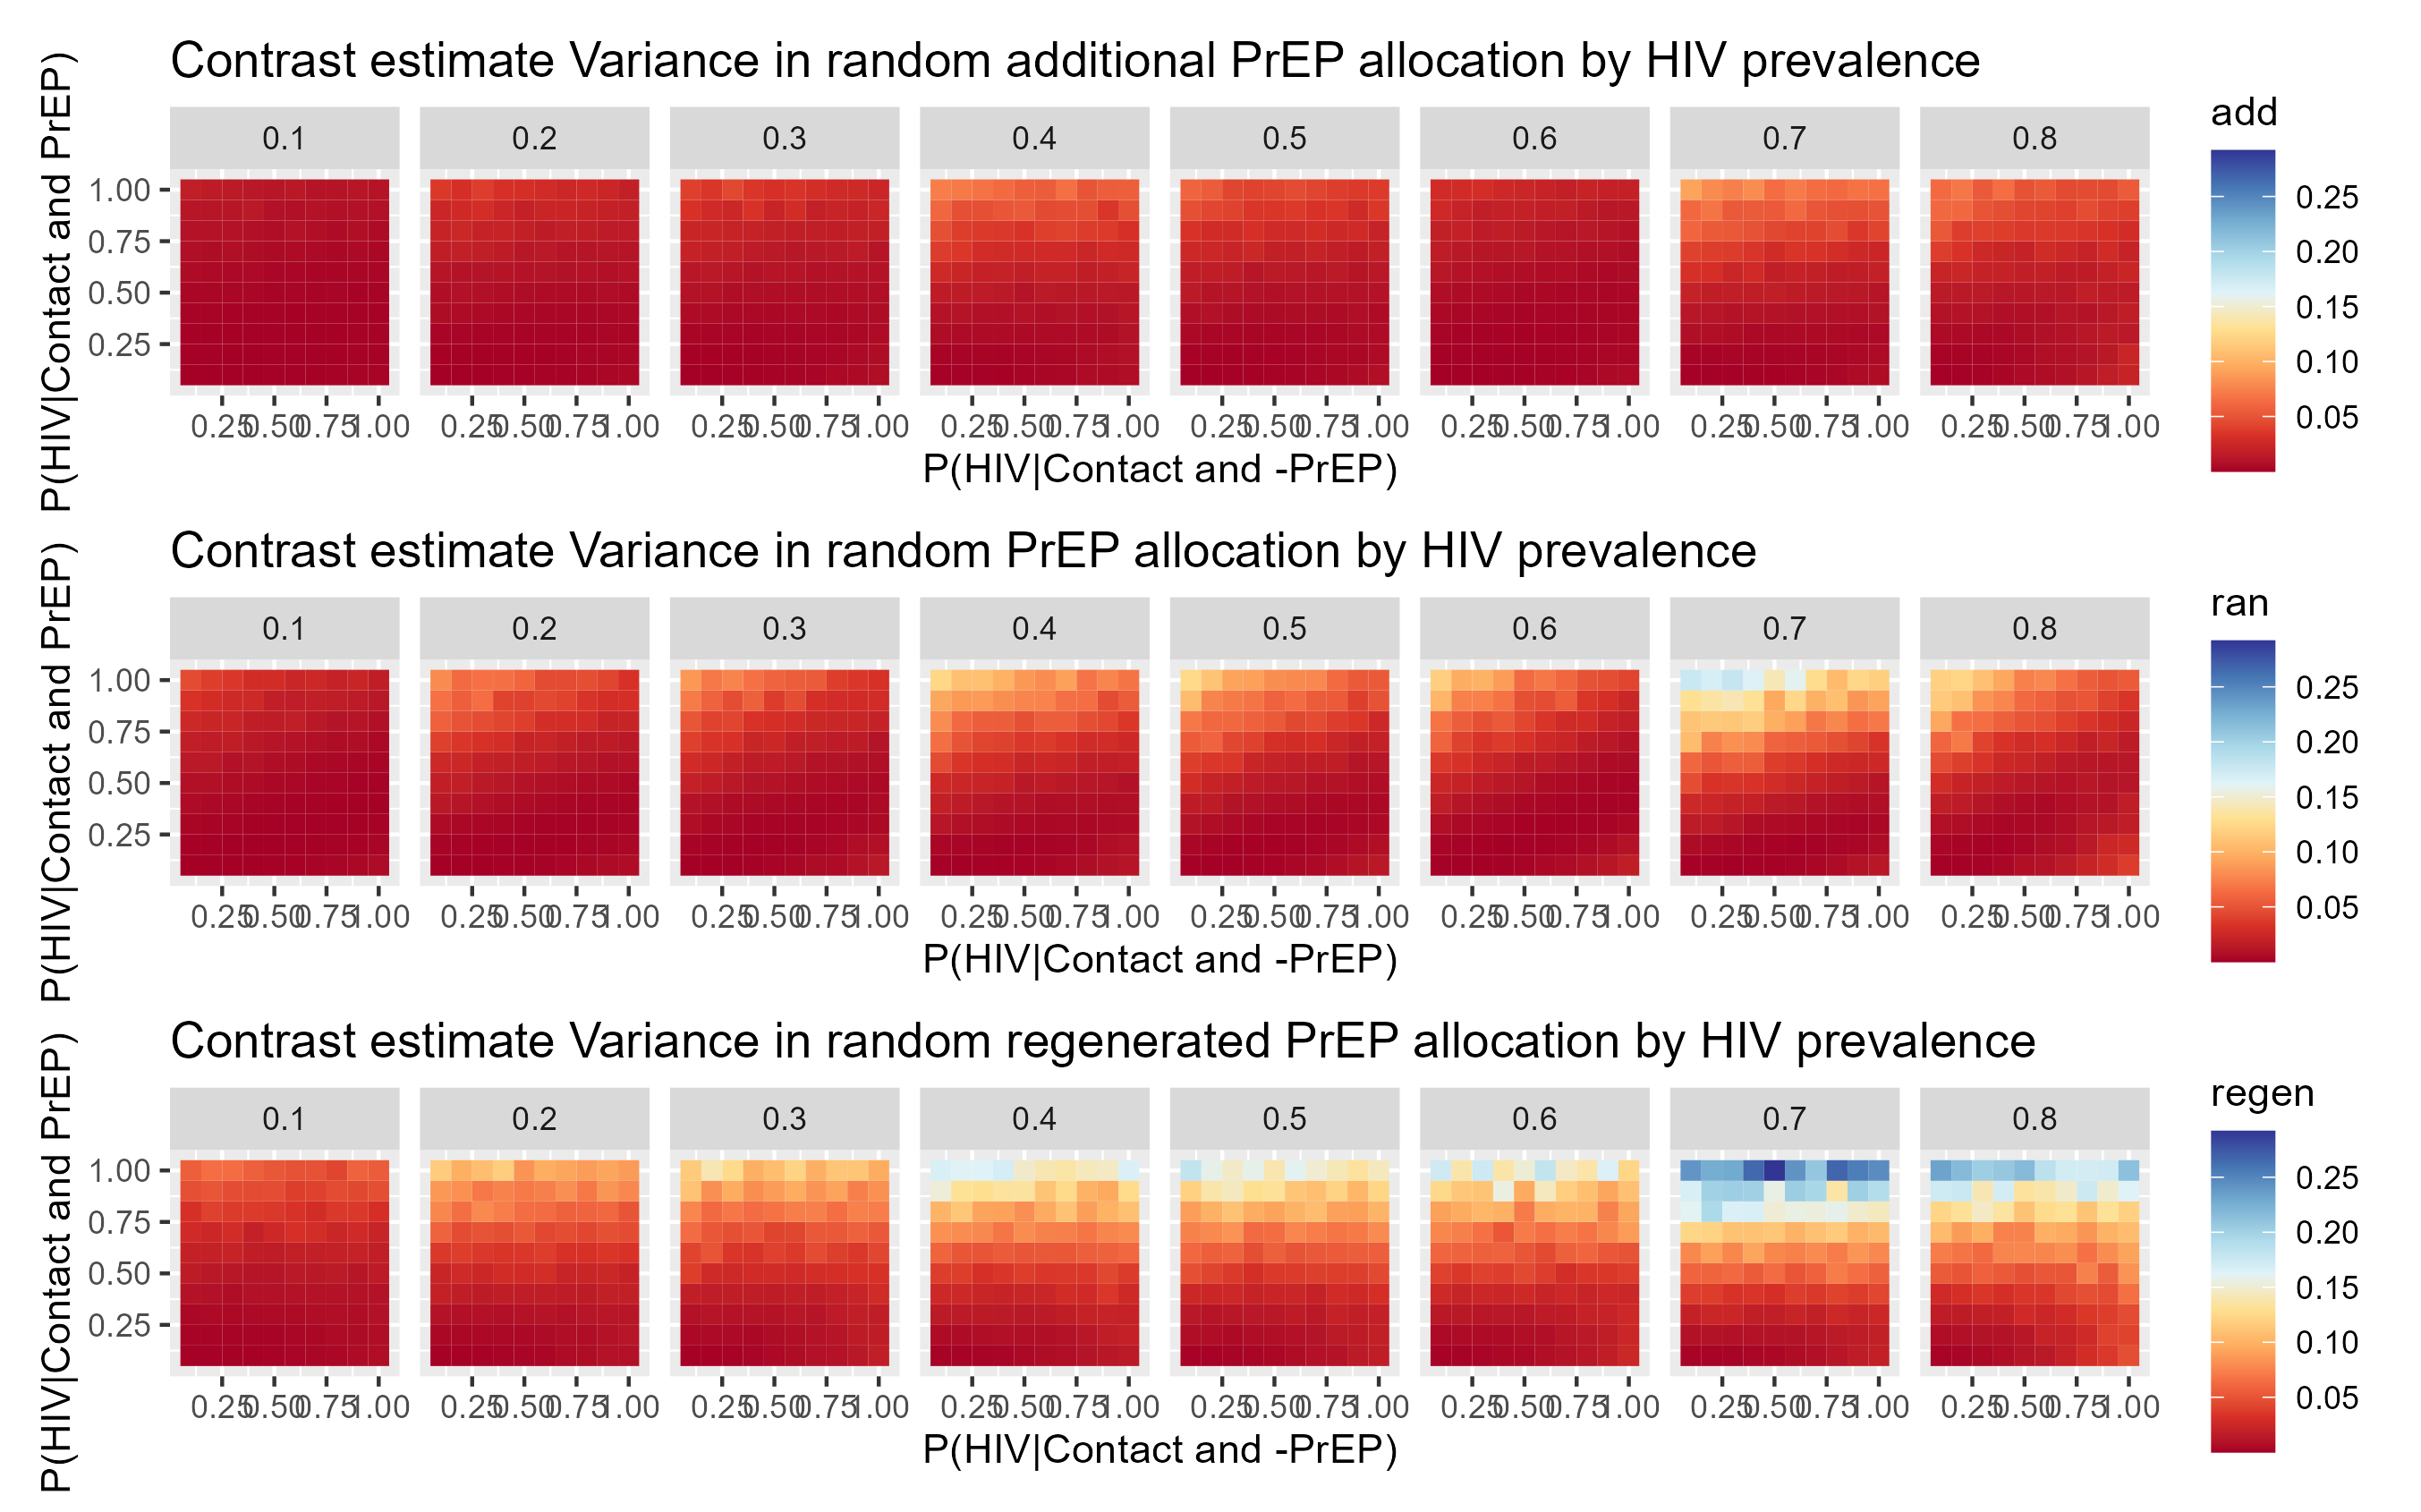
\includegraphics[width=\linewidth]{Figures/HIV Prevalence Variance plots.png}
    \caption{Variance of Causal Contrast estimates as $\mathbb{P}\left[\text{HIV} \vert \neg \text{PrEP} \cap \text{Contact}\right]$ and $\mathbb{P}\left[\text{HIV} \vert \text{PrEP} \cap \text{Contact}\right]$ increase,  stratified by HIV Prevalence. From top to bottom: ``additive" Variance of Contrast of random 20\% additional vs. random 20\% PrEP allocation control, ``random" Variance of Contrast of random 40\% PrEP allocation vs. random 20\% control, ``regenerated" Variance of Contrast of random 40\% allocation on regenerated network vs. random 20\% control.}
    \label{fig:Figure 12}
\end{figure}

While it may be more obvious from the Variance plots in Figure \ref{fig:Figure 12} than in the Mean plots \ref{fig:Figure 11}, there is apparent effect modification of the relationship between underlying HIV risks and treatment strategy by the initial HIV prevalence. We can see three distinct gradients in the magnitude of the contrast estimate Variance over the HIV risks for each of the treatment strategies, with distinct changes in these gradients by HIV prevalence. 
\subsubsection{Effect Modification by \texorpdfstring{$\mathbb{P}[\text{HIV } | \text {Contact } \cap \neg \text{ PrEP}]$}{ℙ[HIV | ¬PrEP]}}
\begin{figure}[H]
    \centering
    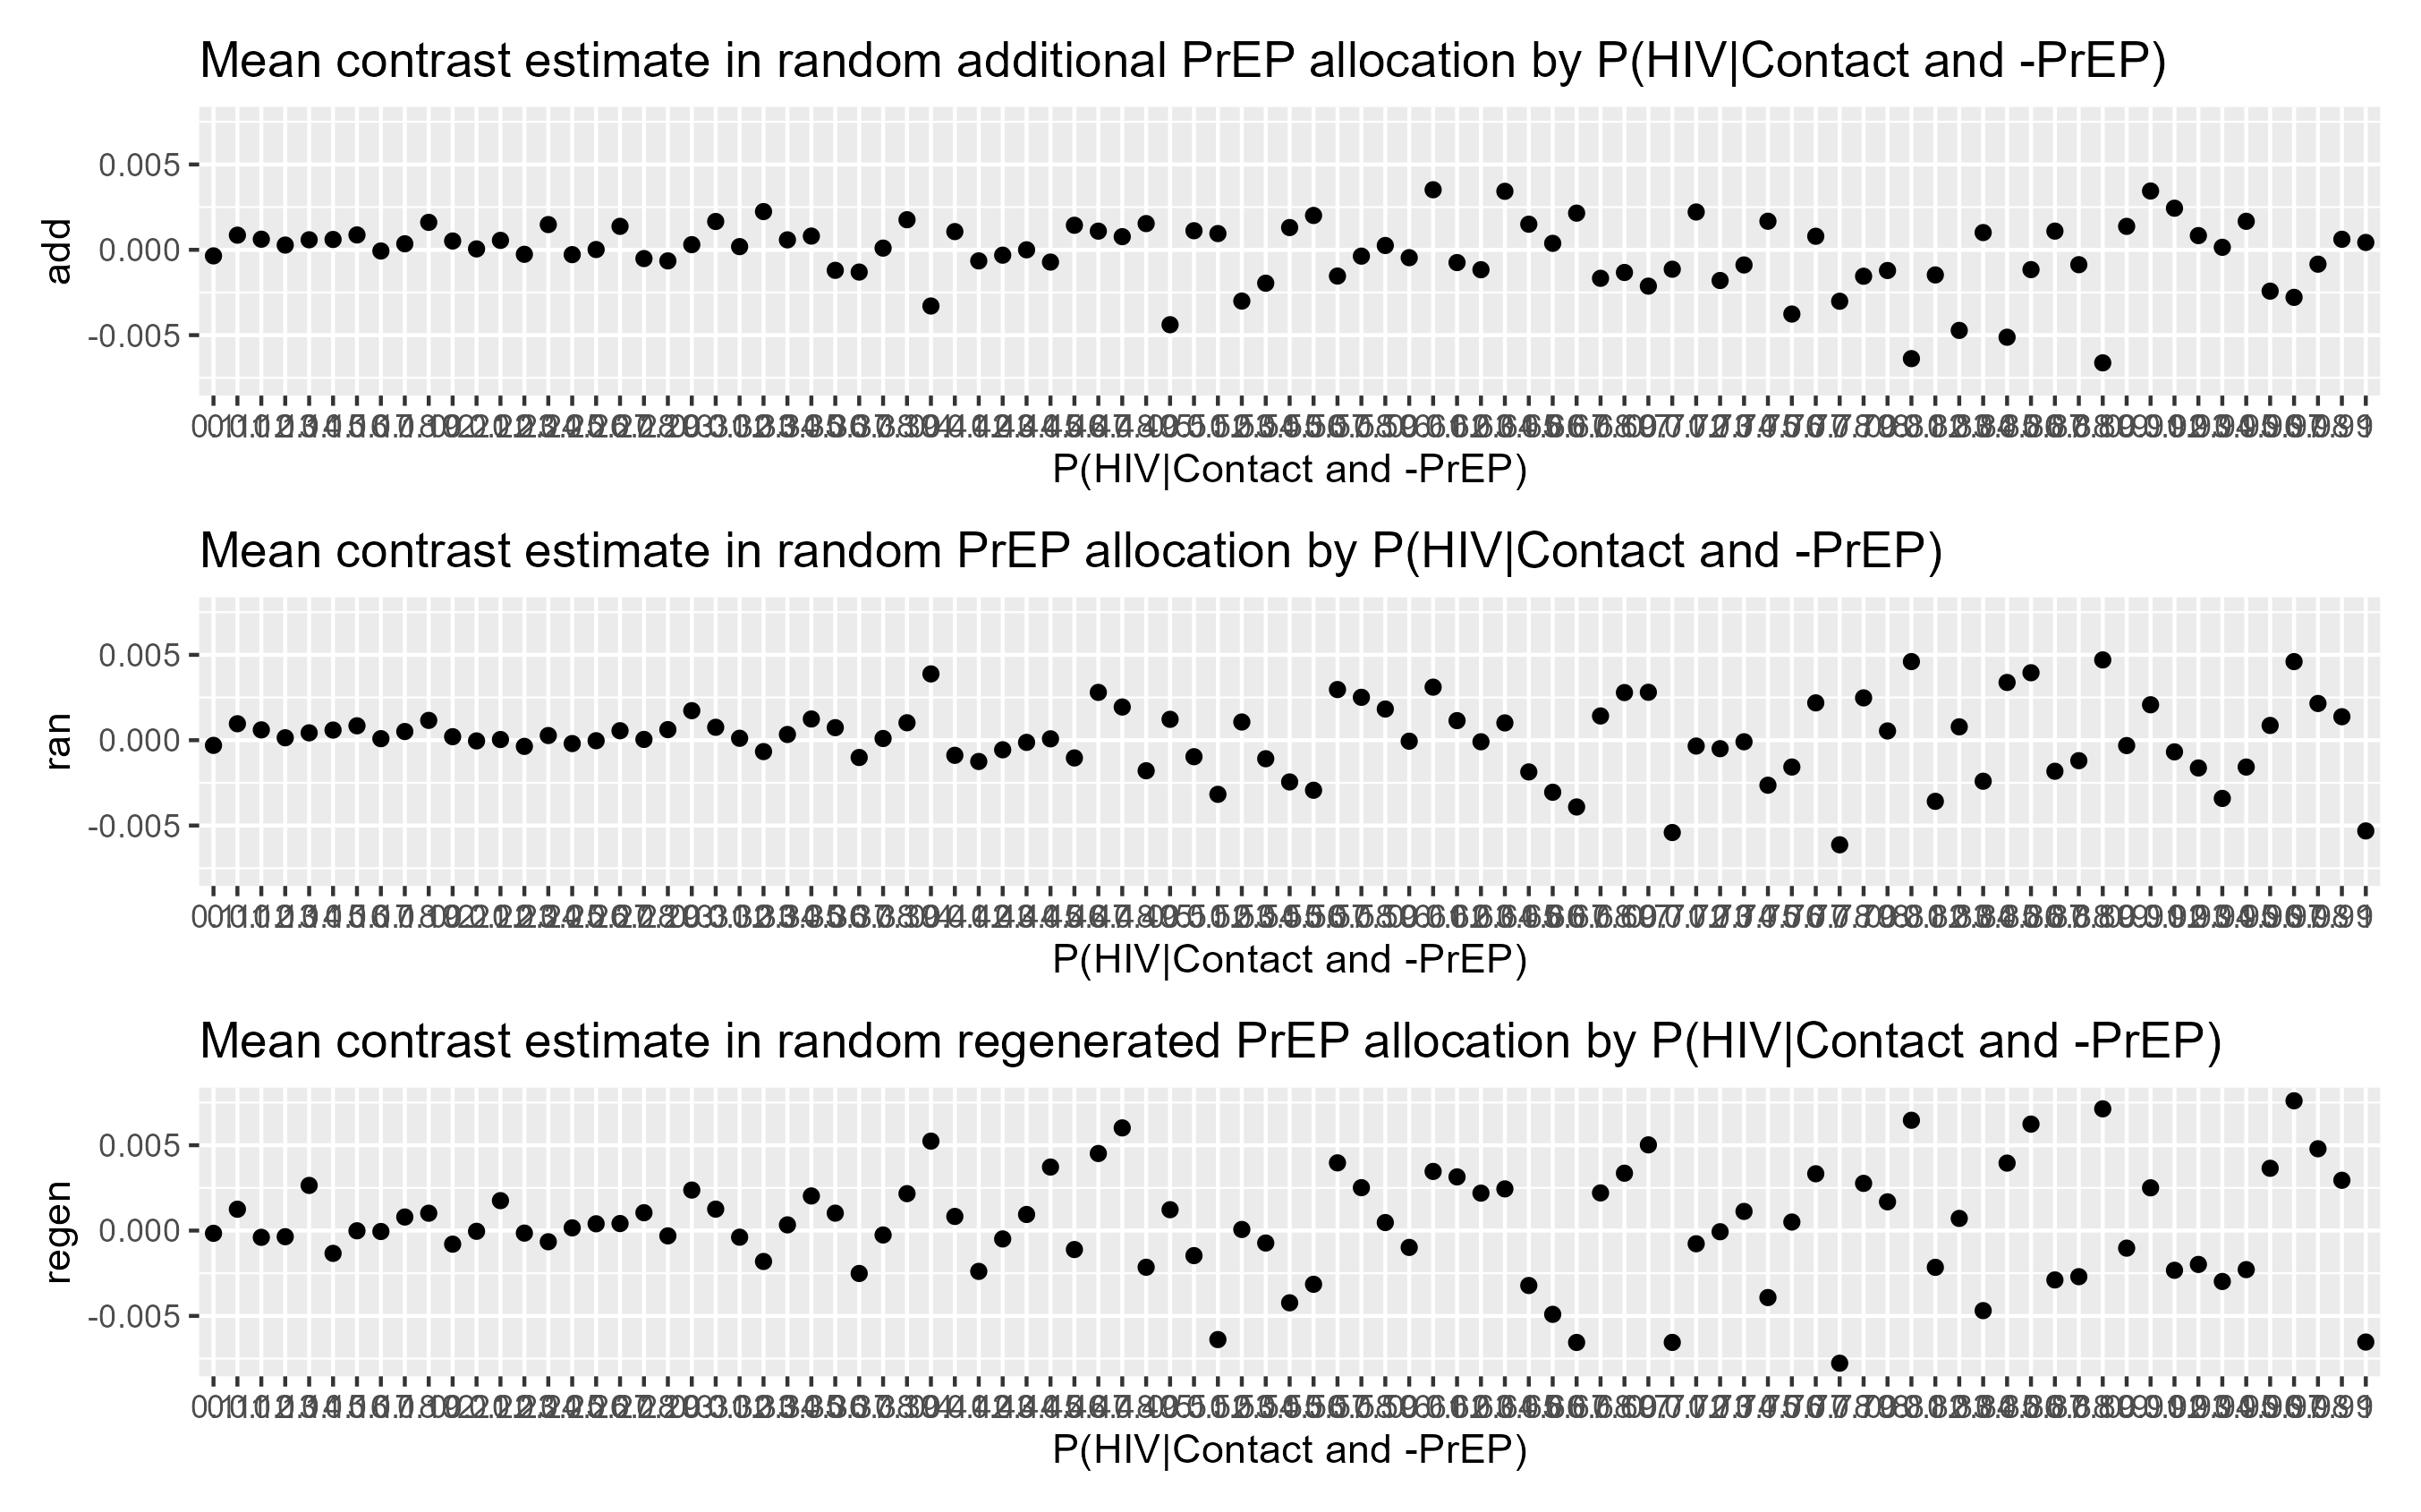
\includegraphics[width=\linewidth]{Figures/p1 Mean plots.png}
    \caption{Mean Causal Contrast estimates as $\mathbb{P}\left[\text{HIV } \vert \text {Contact } \cap \neg \text{ PrEP}\right]$ increases . From top to bottom: ``additive" Mean Contrast of random 20\% additional vs. random 20\% PrEP allocation control, ``random" Mean Contrast of random 40\% PrEP allocation vs. random 20\% control, ``regenerated" Mean Contrast of random 40\% allocation on regenerated network vs. random 20\% control.}
    \label{fig:Figure 13}
\end{figure}
\begin{figure}[H]
    \centering
    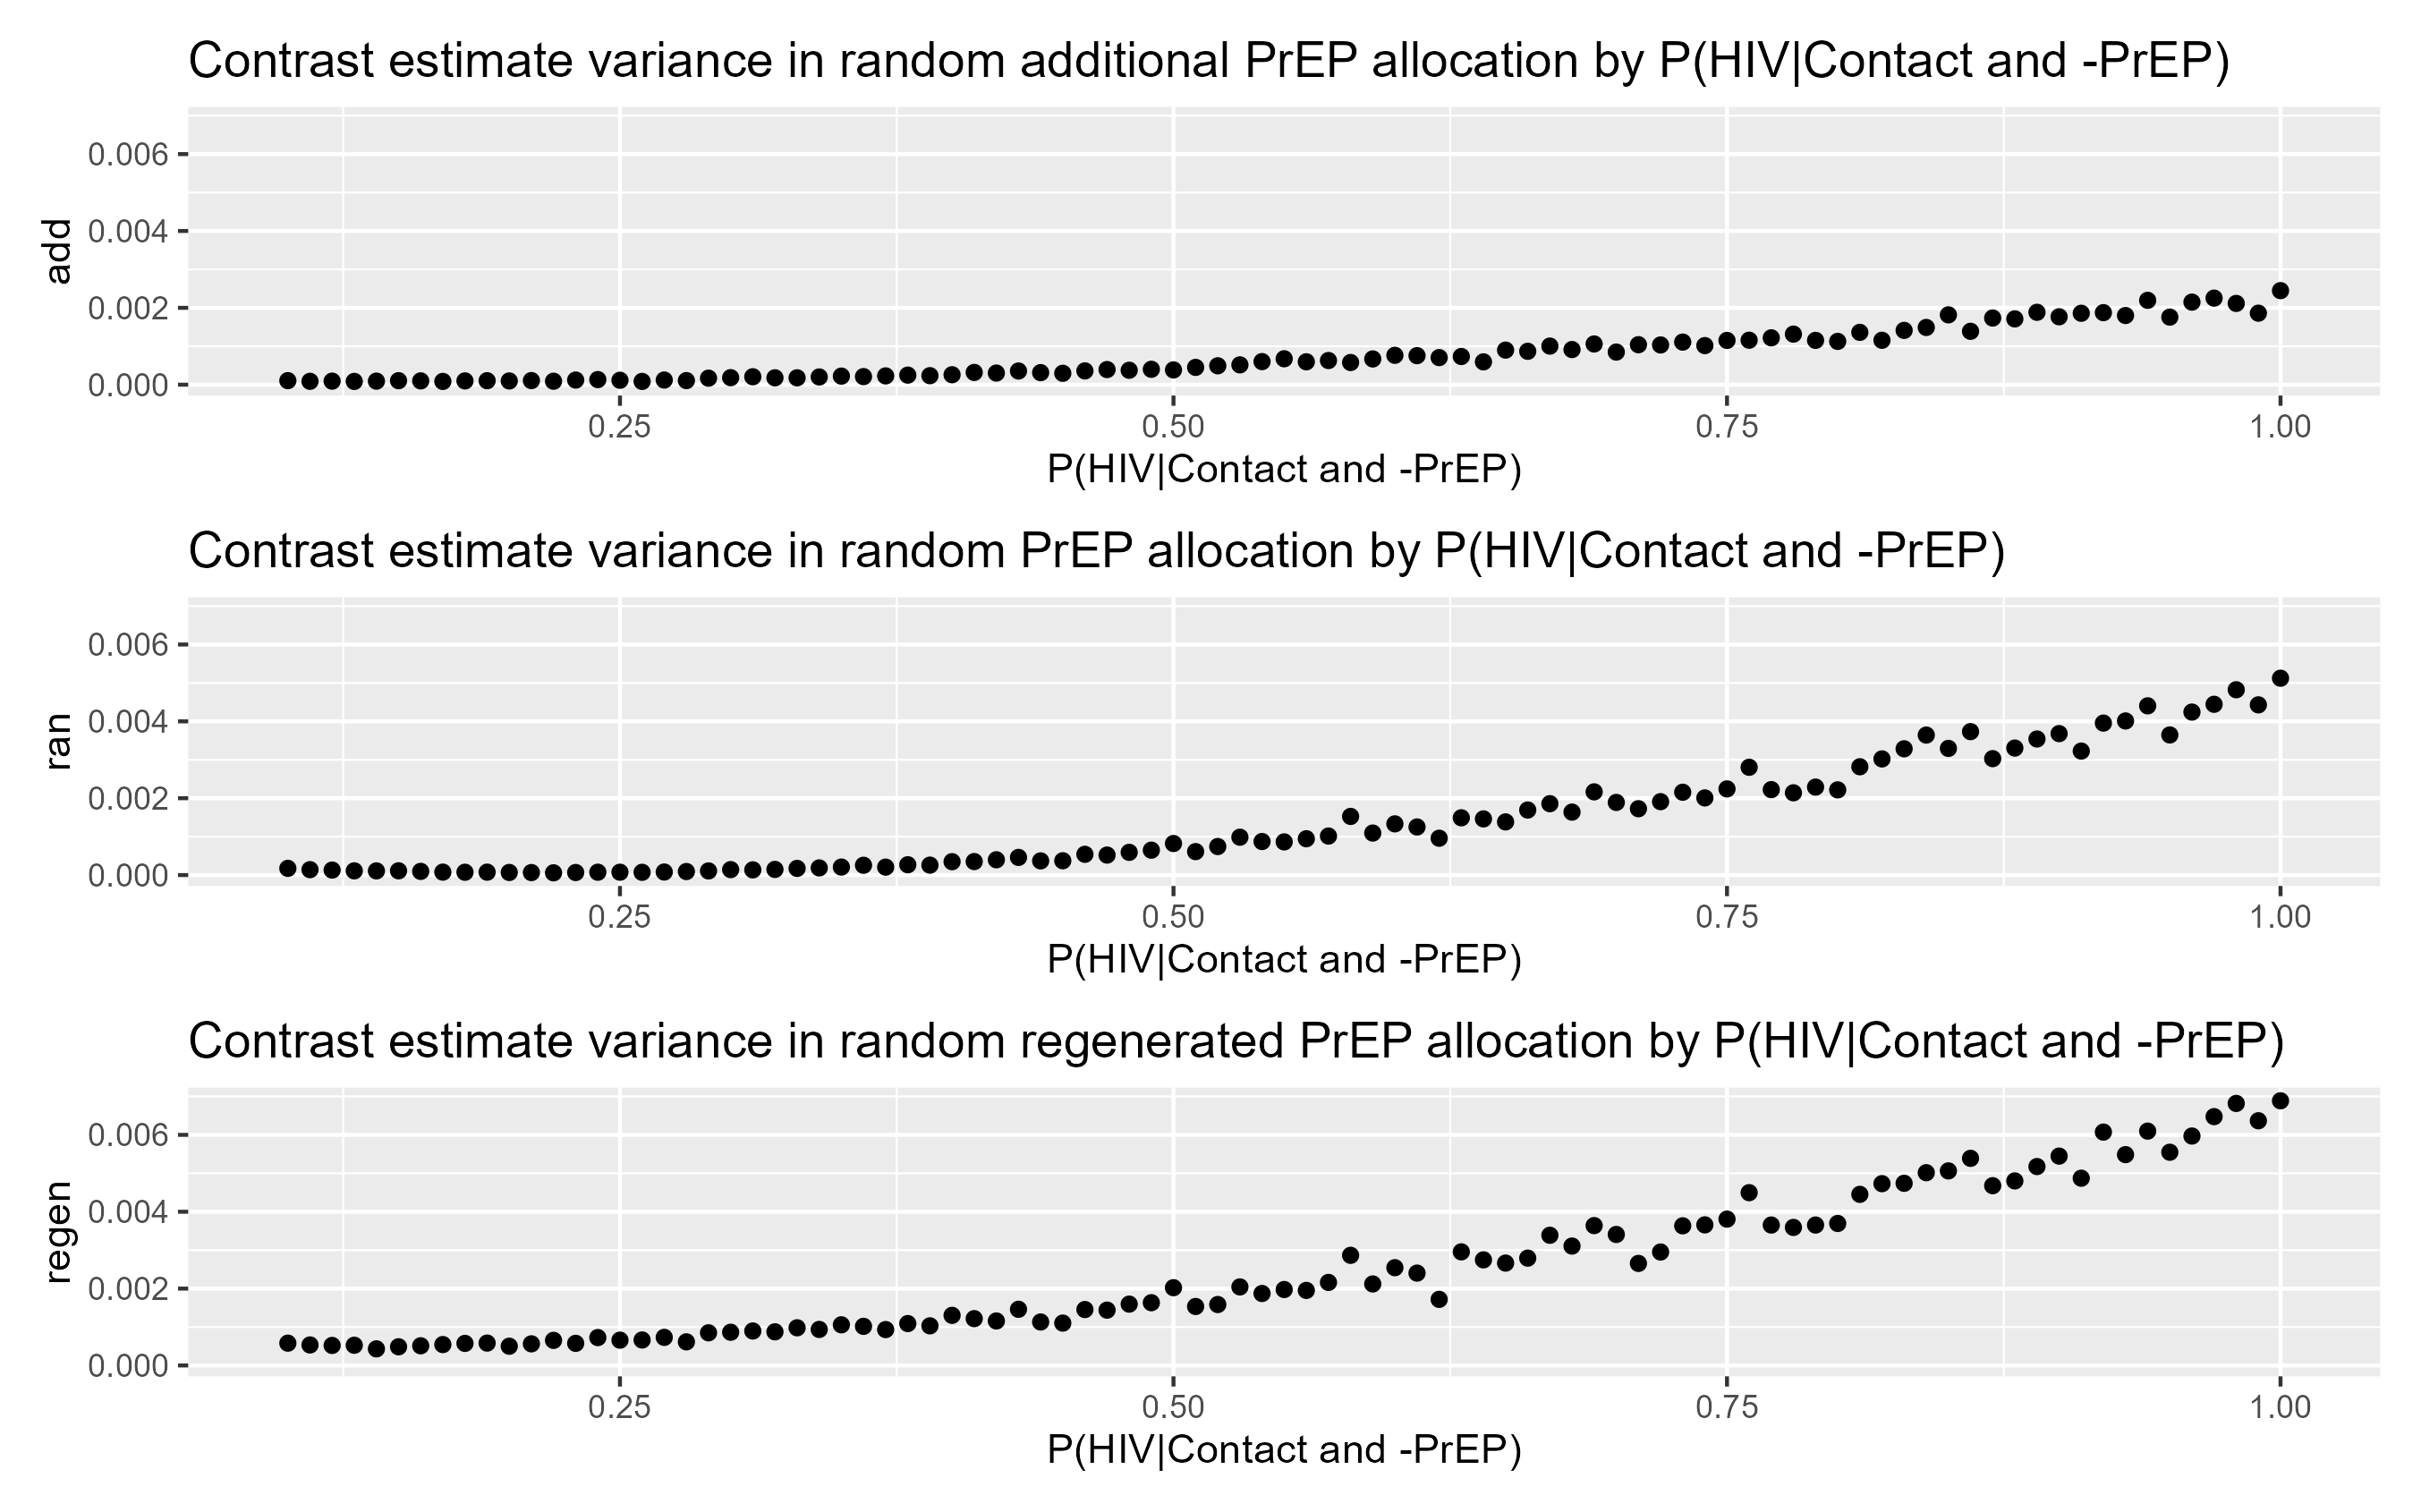
\includegraphics[width=\linewidth]{Figures/p1 Variance plots.png}
    \caption{Variance of Causal Contrast estimates as $\mathbb{P}\left[\text{HIV } \vert \text {Contact } \cap \neg \text{ PrEP}\right]$ increases .  From top to bottom: ``additive" Variance of Contrast of random 20\% additional vs. random 20\% PrEP allocation control, ``random" Variance of Contrast of random 40\% PrEP allocation vs. random 20\% control, ``regenerated" Variance of Contrast of random 40\% allocation on regenerated network vs. random 20\% control.}
    \label{fig:Figure 14}
\end{figure}
From the contrast estimate Mean and Variance plots in figures \ref{fig:Figure 13} and \ref{fig:Figure 14} above, we observe effect modification of the relationship between the underlying risk of HIV given contact and no treatment and HIV risk by treatment strategy. Whilst in the ``additive" treatment strategy, the contrast estimate Mean and Variance are both very small and relatively constant except for relatively large values of $\mathbb{P}\left[\text{HIV } \vert \text {Contact } \cap \neg \text{ PrEP}\right]$. The ``random" and ``regenerated" treatment strategies show marked heteroskedasticity beginning with much smaller values of $\mathbb{P}\left[\text{HIV } \vert \text {Contact } \cap \neg \text{ PrEP}\right]$, with the "regenerated" strategy usually having larger variability than the ``random" strategy for the same value of $\mathbb{P}\left[\text{HIV } \vert \text {Contact } \cap \neg \text{ PrEP}\right]$.  
\subsubsection{Effect Modification by \texorpdfstring{$\mathbb{P}\left[\text{HIV } \vert \text {Contact } \cap \text{ PrEP}\right]$}{ℙ[HIV | PrEP]}}
\begin{figure}[H]
    \centering
    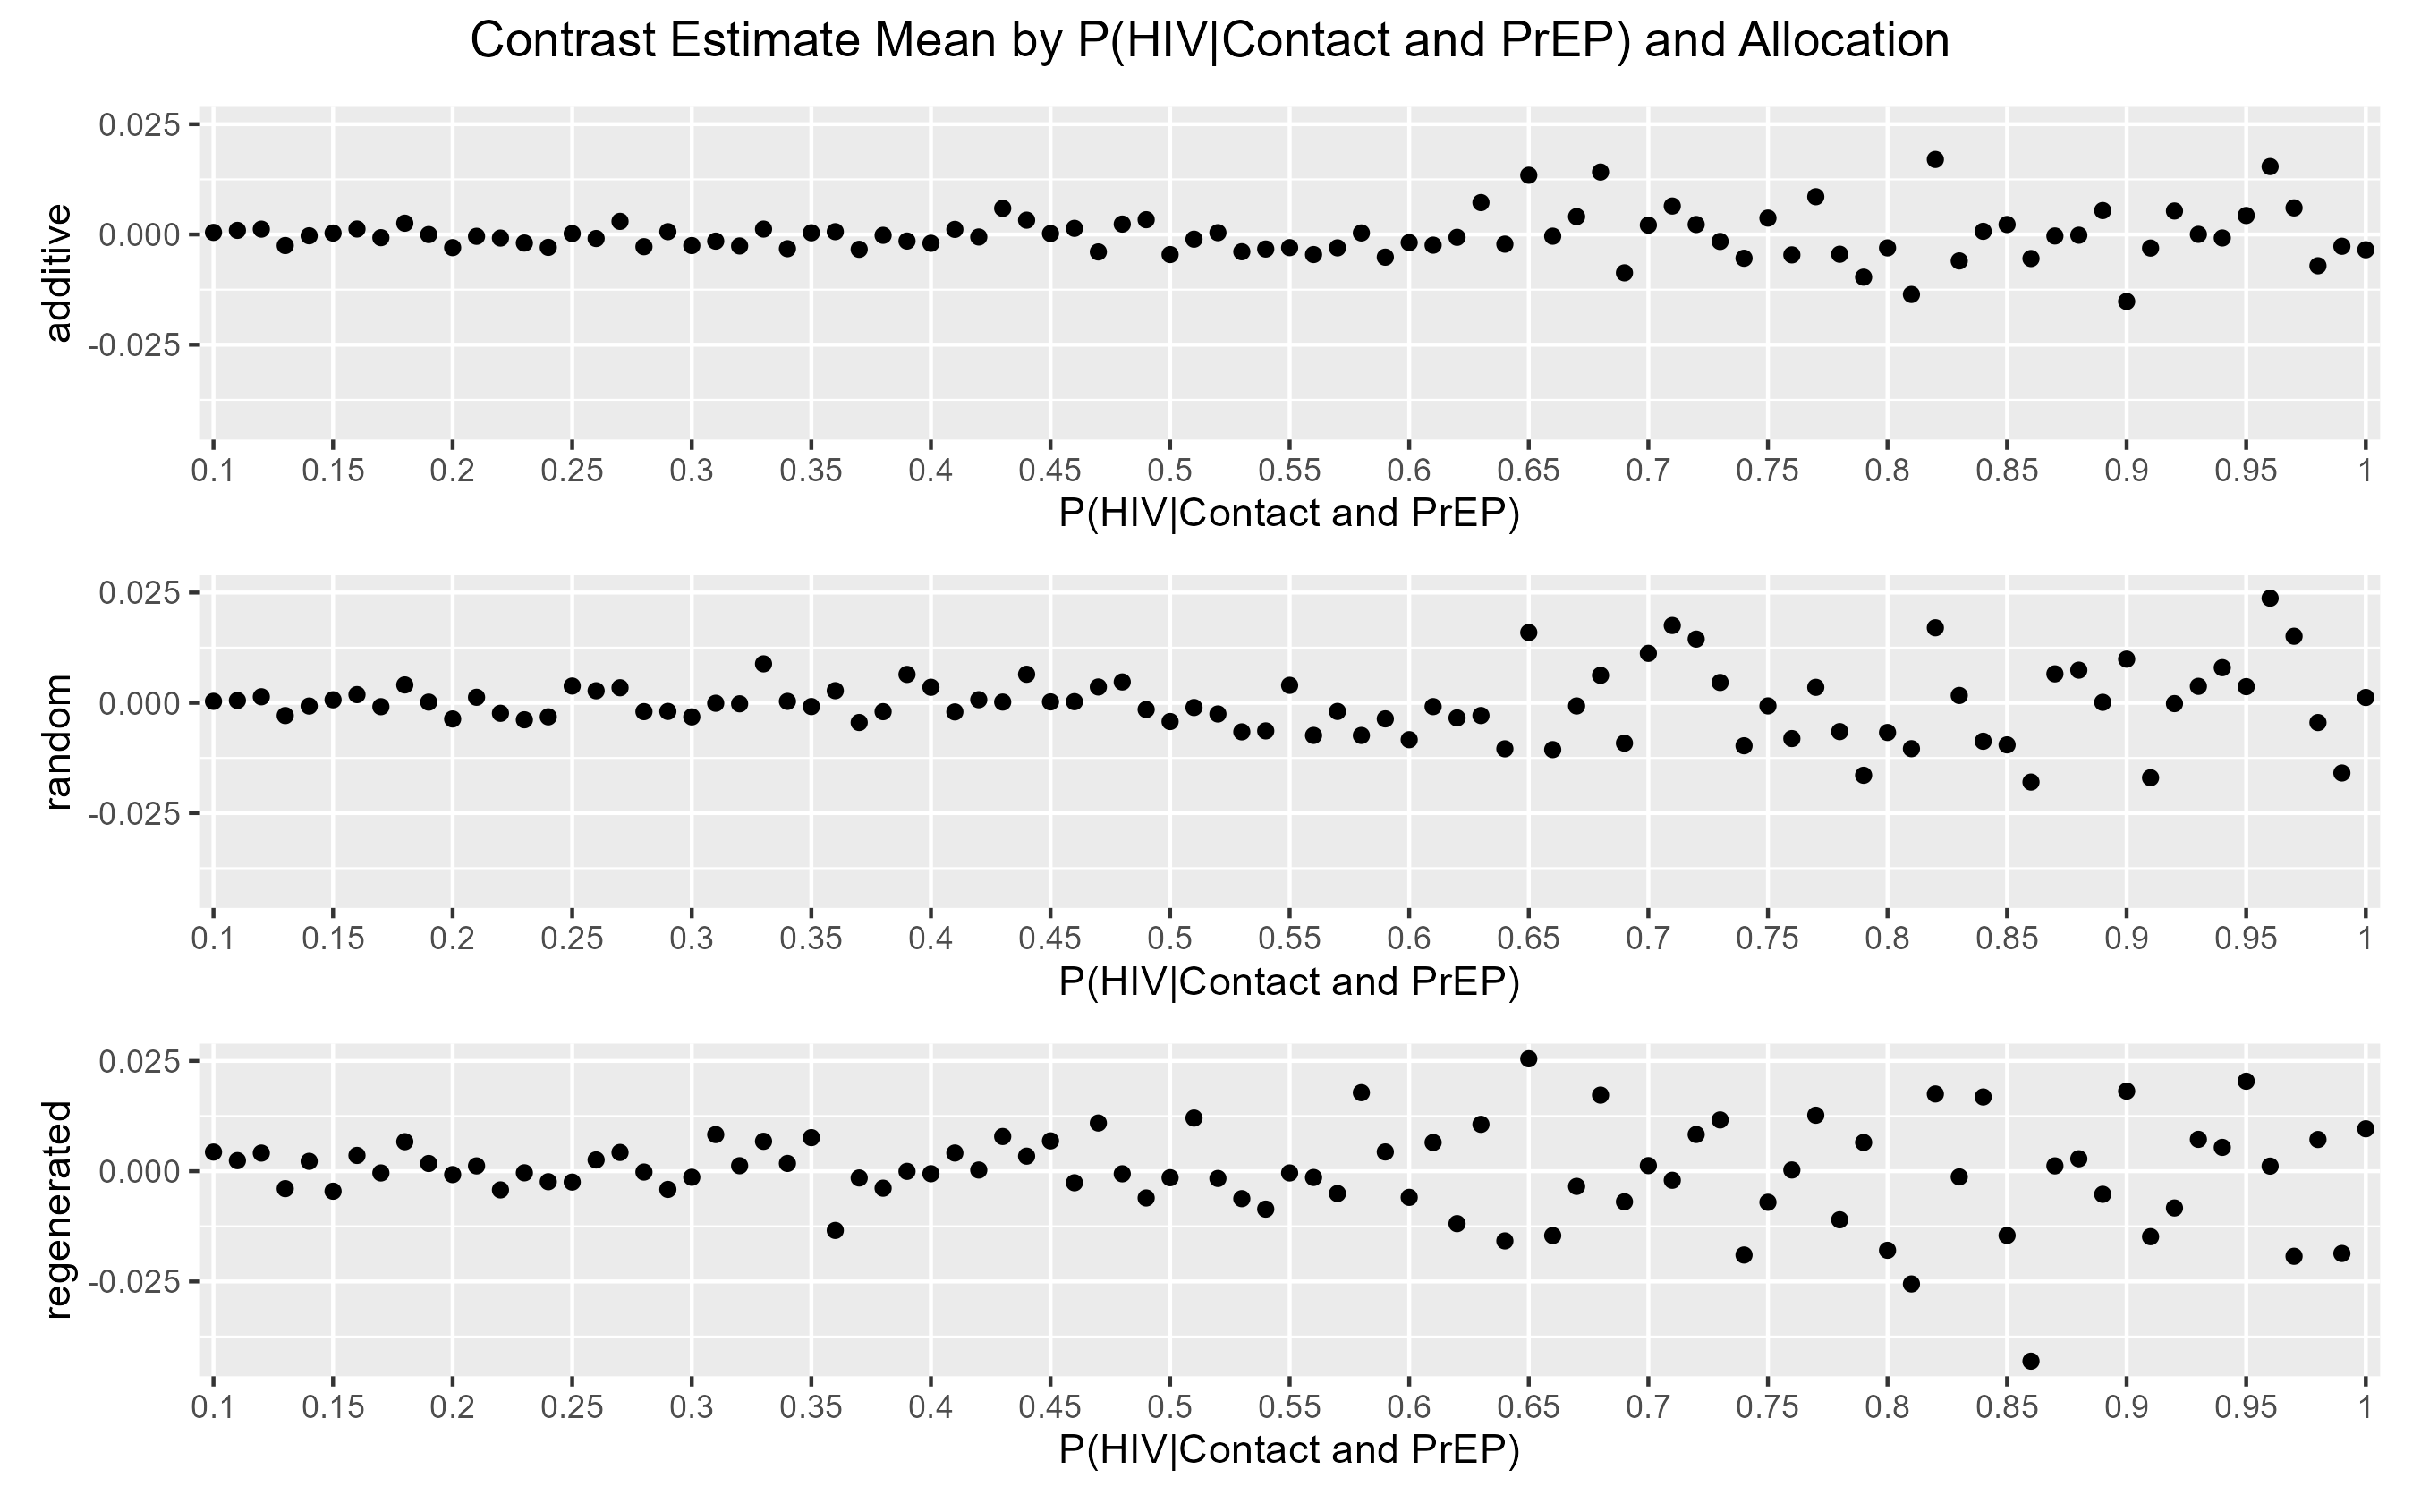
\includegraphics[width=\linewidth]{Figures/p2 Mean plots.png}
    \caption{Mean Causal Contrast estimates as $\mathbb{P}\left[\text{HIV } \vert \text{ PrEP}\right]$ increases . From top to bottom: ``additive" Mean Contrast of random 20\% additional vs. random 20\% PrEP allocation control, ``random" Mean Contrast of random 40\% PrEP allocation vs. random 20\% control, ``regenerated" Mean Contrast of random 40\% allocation on regenerated network vs. random 20\% control.}
    \label{fig:Figure 15}

\end{figure}

\begin{figure}[H]
    \centering
    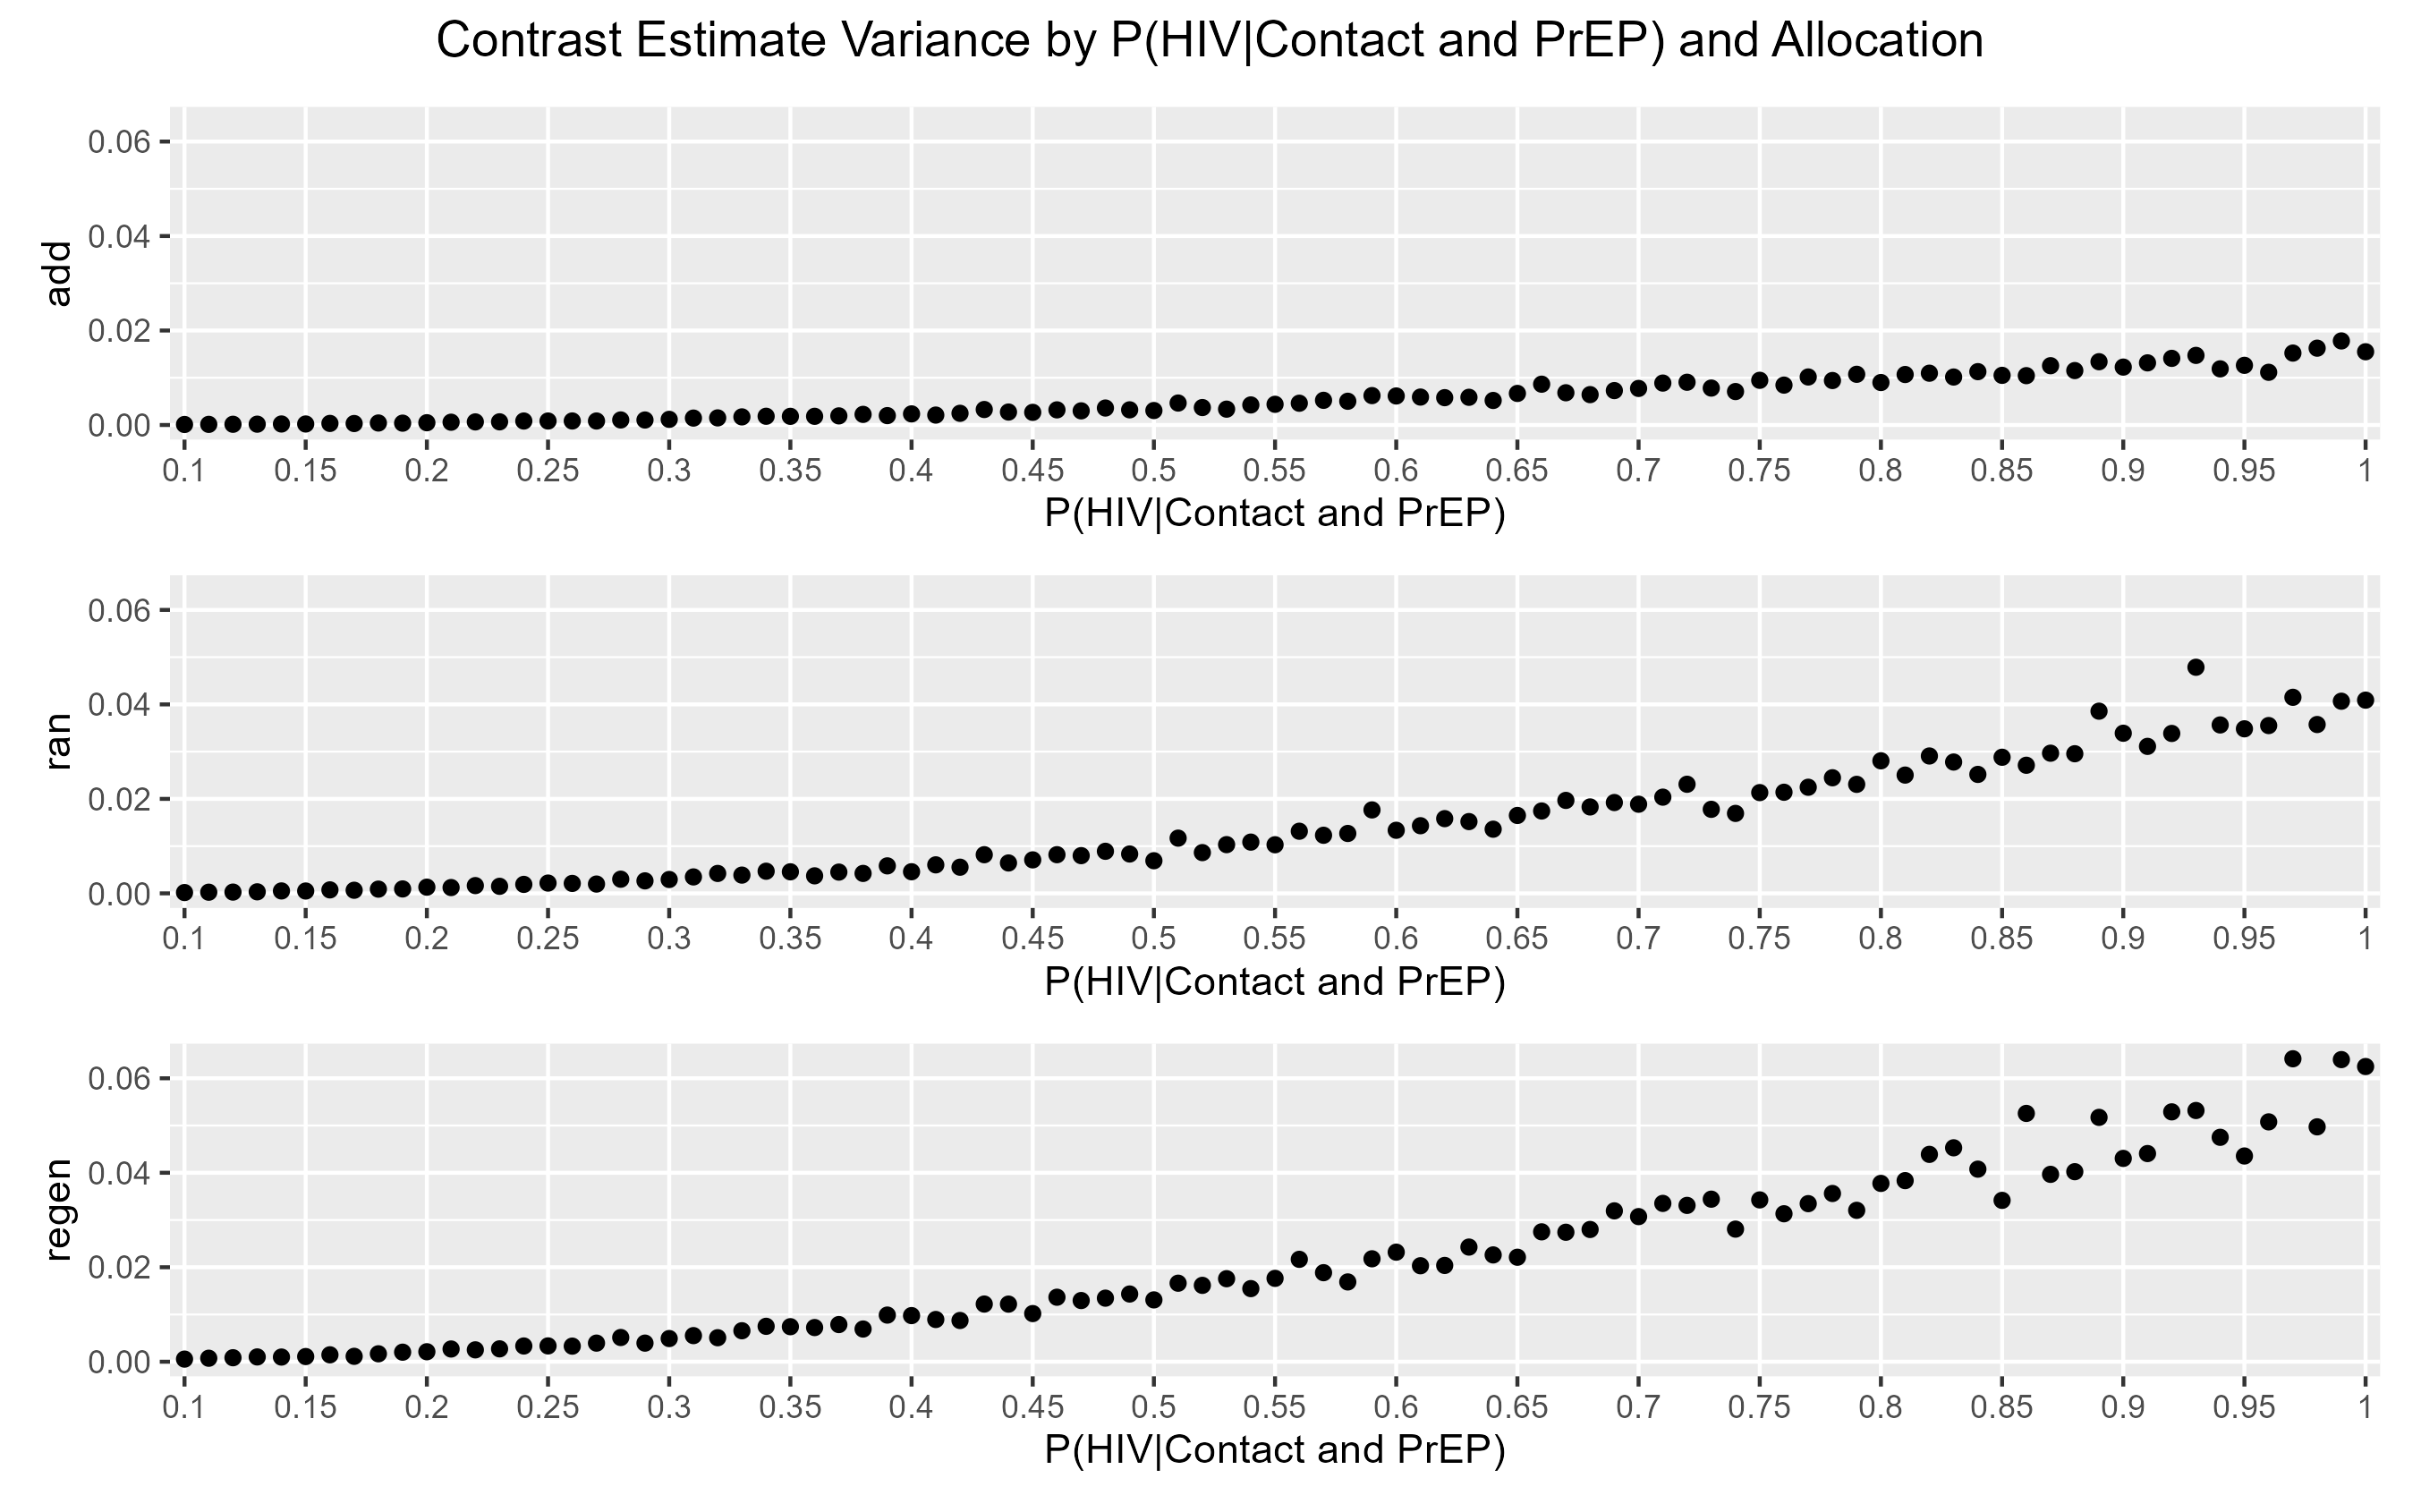
\includegraphics[width=\linewidth]{Figures/p2 Variance plots.png}
    \caption{Variance of Causal Contrast estimates as $\mathbb{P}\left[\text{HIV } \vert \text{ PrEP}\right]$ increases .  From top to bottom: ``additive" Variance of Contrast of random 20\% additional vs. random 20\% PrEP allocation control, ``random" Variance of Contrast of random 40\% PrEP allocation vs. random 20\% control, ``regenerated" Variance of Contrast of random 40\% allocation on regenerated network vs. random 20\% control.}
    \label{fig:Figure 16}
\end{figure}
Much like with the underlying risk of HIV given no treatment, we observe effect modification of the relationship between the underlying risk of HIV given infectious contact and PrEP treatment by allocation strategy. This modification is apparent in both Causal Contrast estimate Mean and Variance plots in Figure \ref{fig:Figure 15} and \ref{fig:Figure 16}, respectively. While the modification is qualitatively similar to that for the no treatment risk, it is interesting to note that the range of both Mean and Variance magnitudes is larger for $\mathbb{P}\left[\text{HIV } \vert \text{ PrEP}\right]$ than for $\mathbb{P}\left[\text{HIV } \vert \text {Contact } \cap \neg \text{ PrEP}\right]$.

\subsubsection{Effect Modification by PrEP contrasts in ER model}
\begin{figure}[H]
    \centering
    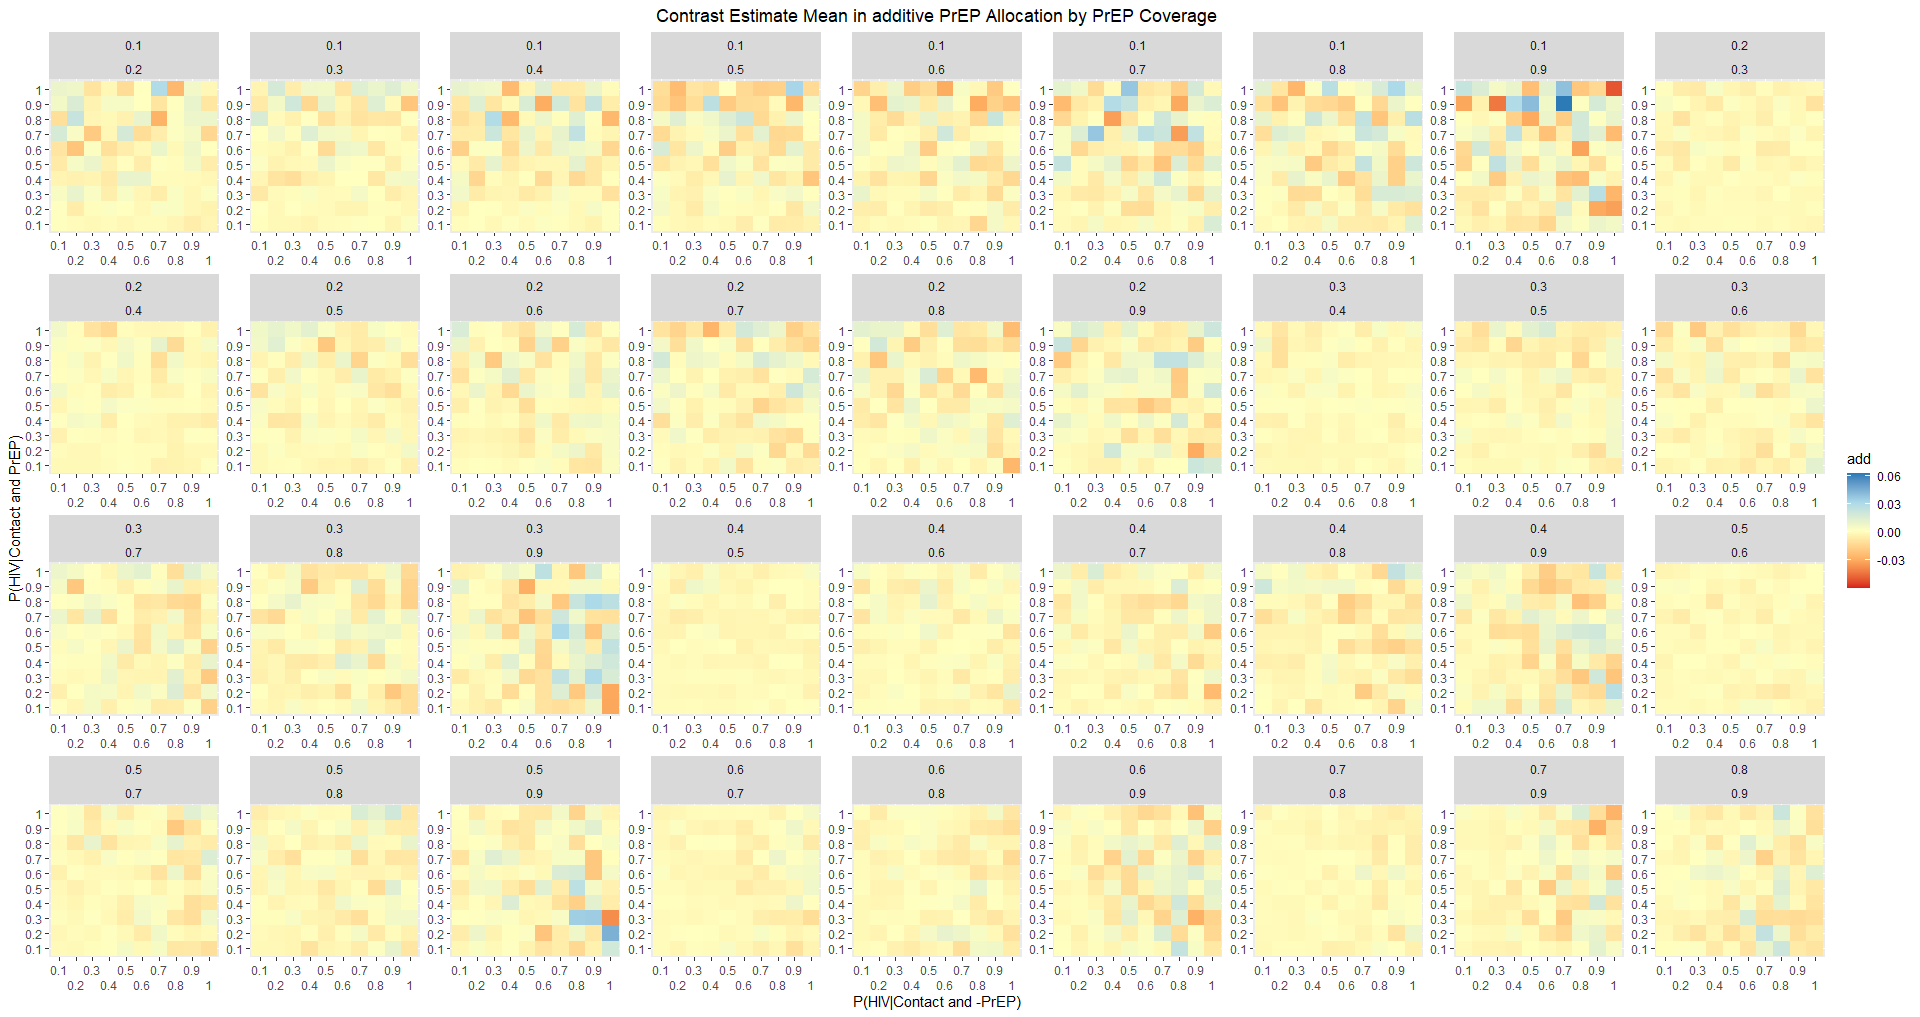
\includegraphics[width=\linewidth]{Figures/PrEP Additive Mean Plots.png}
    \caption{Mean Causal Contrast estimates as $\mathbb{P}\left[\text{HIV} \vert \neg \text{PrEP} \cap \text{Contact}\right]$ and $\mathbb{P}\left[\text{HIV} \vert \text{PrEP} \cap \text{Contact}\right]$ increase, stratified by random PrEP1\% additional vs. random PrEP2-PrEP1 \% PrEP allocation control. Top number indicates PrEP1 \% control coverage. Bottom number is PrEP2 counterfactual coverage. }
    \label{fig:Figure 17}
\end{figure}
\begin{figure}[H]
    \centering
    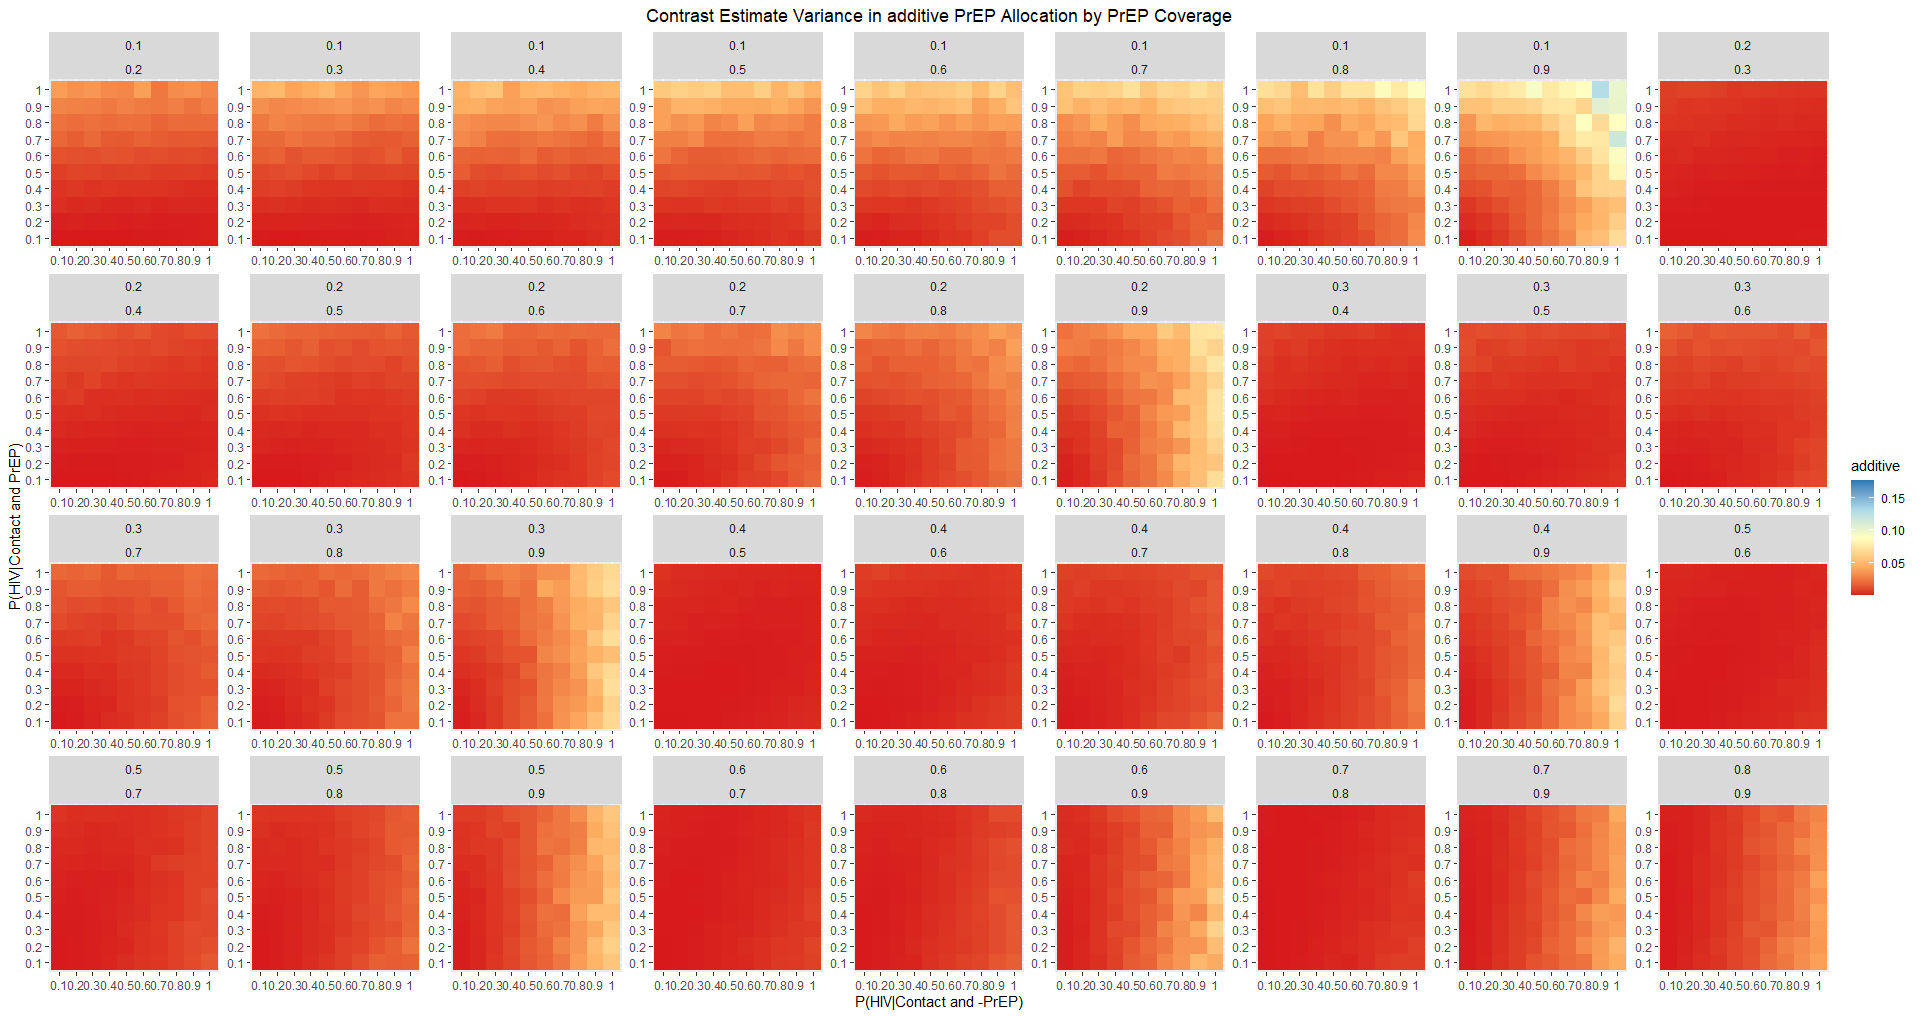
\includegraphics[width=\linewidth]{Figures/PrEP Additive Variance Plots.png}
    \caption{Variance of Causal Contrast estimates as $\mathbb{P}\left[\text{HIV} \vert \neg \text{PrEP} \cap \text{Contact}\right]$ and $\mathbb{P}\left[\text{HIV} \vert \text{PrEP} \cap \text{Contact}\right]$ increase, stratified by random PrEP2-PrEP1\% additional vs. random PrEP1 \% PrEP allocation control. Top number indicates PrEP1/control coverage. Bottom number is PrEP2 counterfactual coverage.}
    \label{fig:Figure 18}
\end{figure}
\begin{figure}[H]
    \centering
    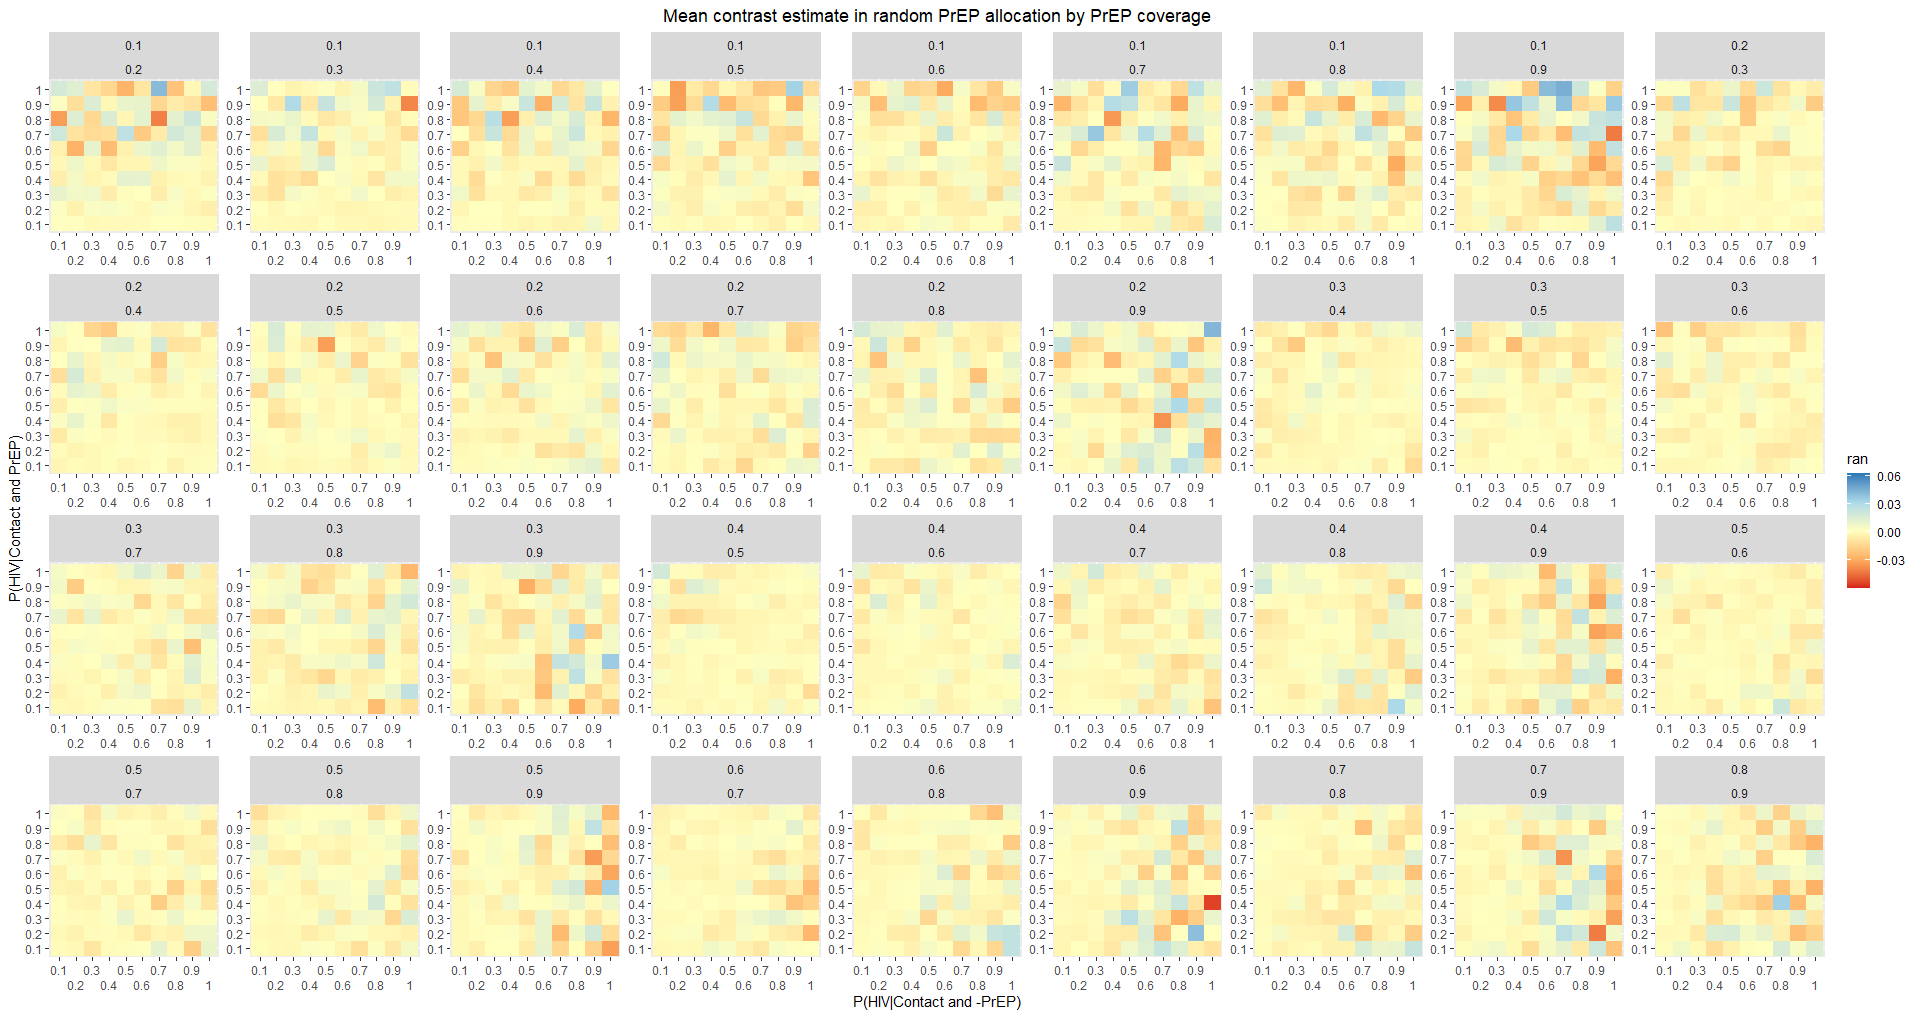
\includegraphics[width=\linewidth]{Figures/PrEP Random Mean Plots.png}
    \caption{Mean Causal Contrast estimates as $\mathbb{P}\left[\text{HIV} \vert \neg \text{PrEP} \cap \text{Contact}\right]$ and $\mathbb{P}\left[\text{HIV} \vert \text{PrEP} \cap \text{Contact}\right]$ increase, stratified by random PrEP2\% vs. random PrEP1\% PrEP allocation control. Top number indicates PrEP1/control coverage. Bottom number is PrEP2 counterfactual coverage.}
    \label{fig:Figure 19}
\end{figure}
\begin{figure}[H]
    \centering
    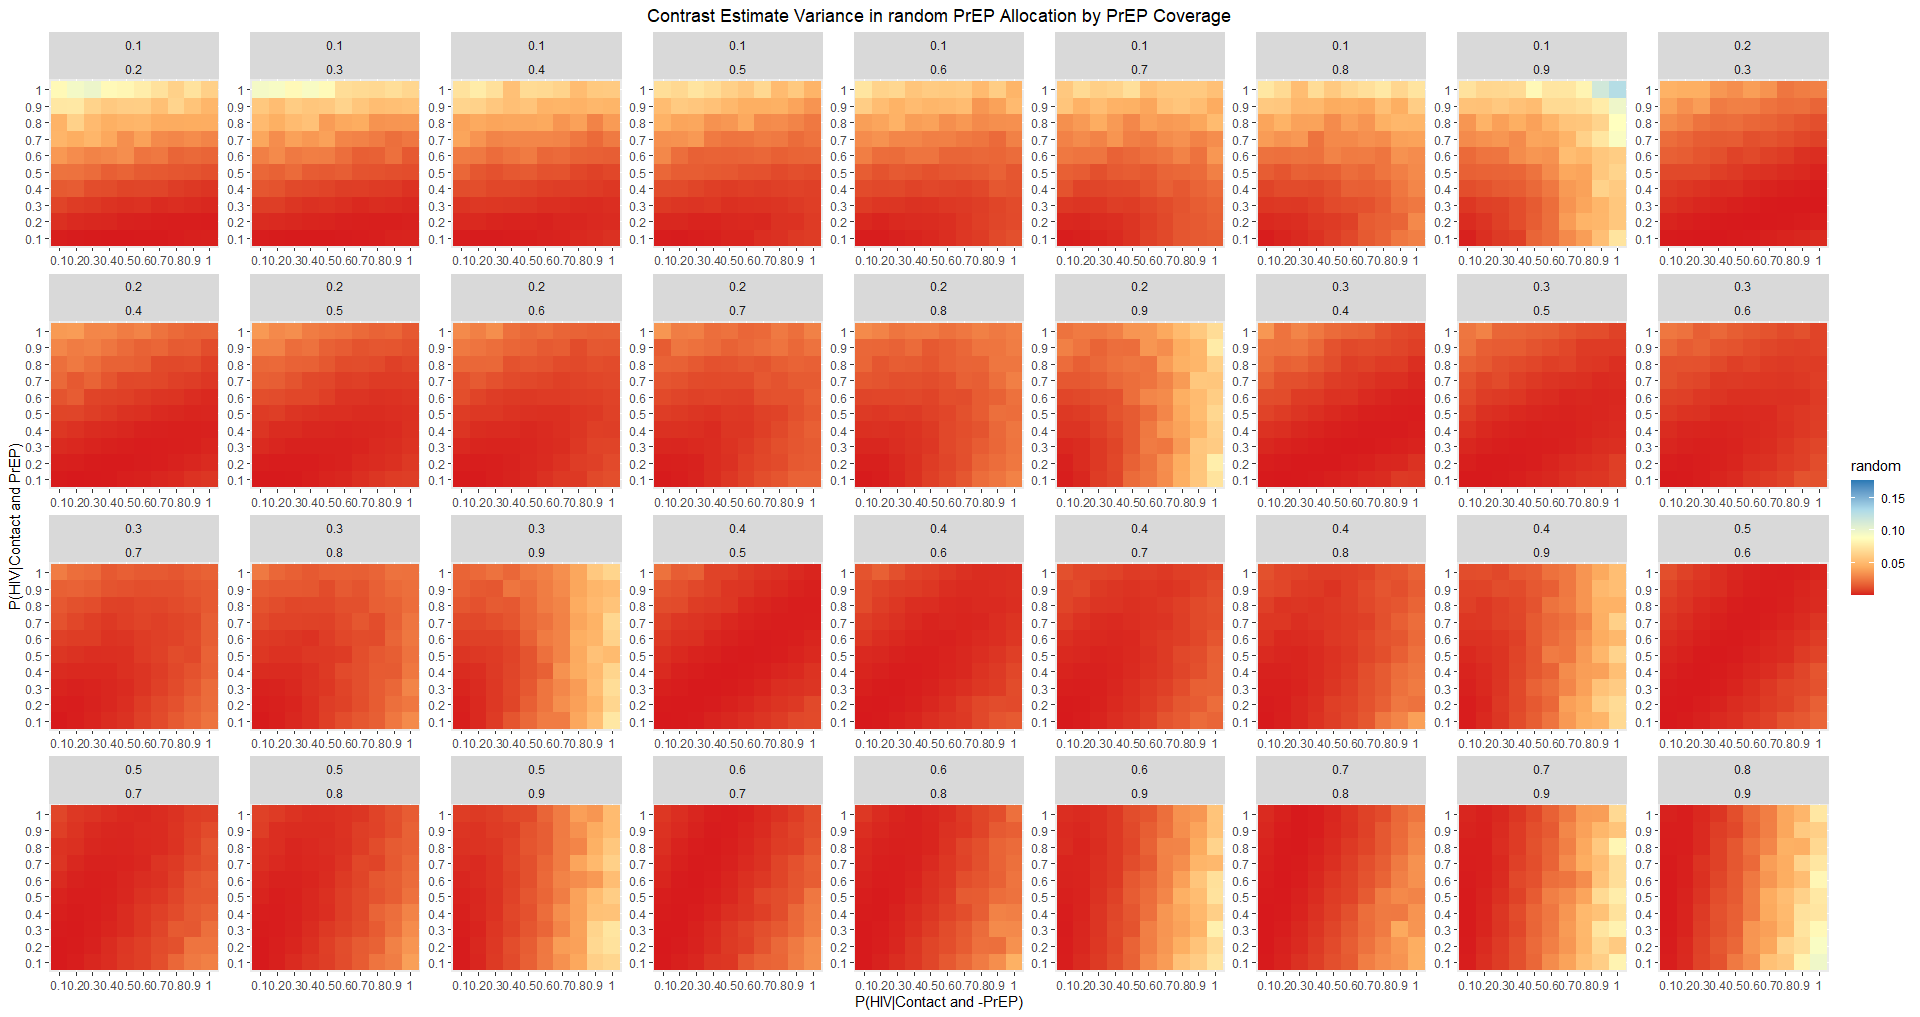
\includegraphics[width=\linewidth]{Figures/PrEP Random Variance Plots.png}
    \caption{Variance of Causal Contrast estimates as $\mathbb{P}\left[\text{HIV} \vert \neg \text{PrEP} \cap \text{Contact}\right]$ and $\mathbb{P}\left[\text{HIV} \vert \text{PrEP} \cap \text{Contact}\right]$ increase, stratified by random PrEP2\% vs. random PrEP1\% PrEP allocation control. Top number indicates PrEP1/control coverage. Bottom number is PrEP2 counterfactual coverage.}
    \label{fig:Figure 20}
\end{figure}
\begin{figure}[H]
    \centering
    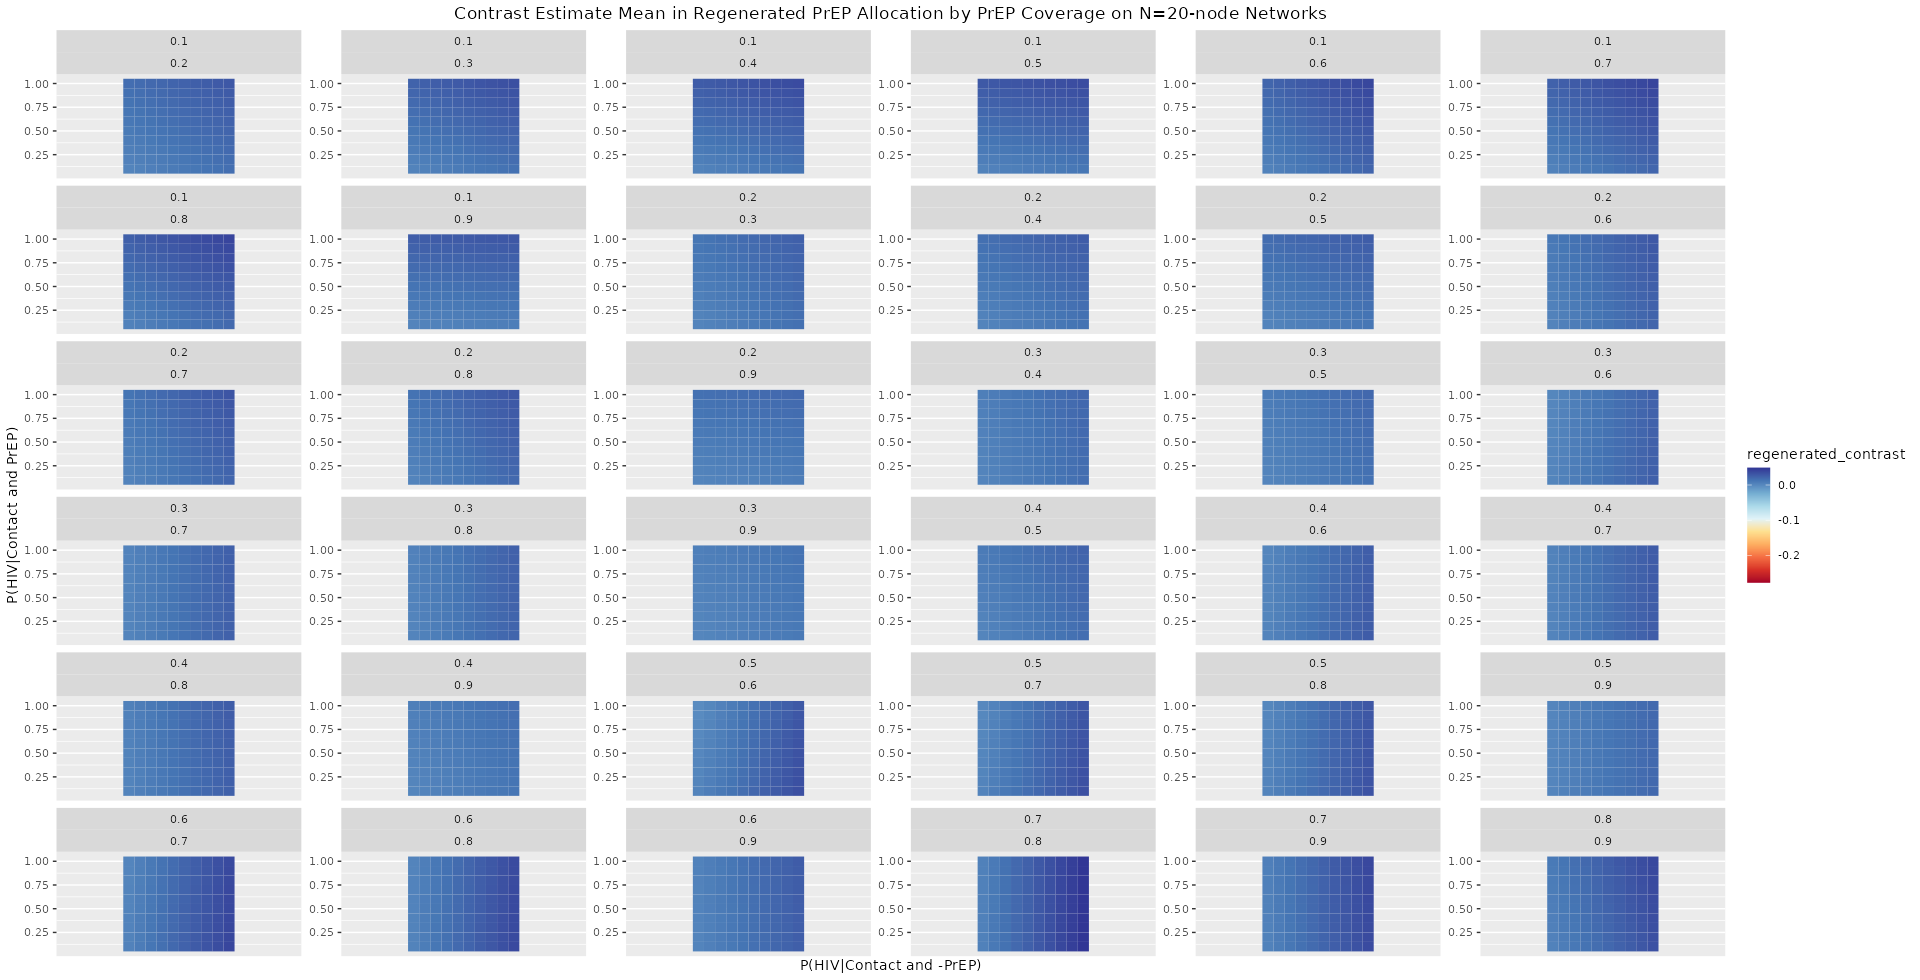
\includegraphics[width=\linewidth]{Figures/PrEP Regenerated Mean Plots.png}
    \caption{Mean of Causal Contrast estimates as $\mathbb{P}\left[\text{HIV} \vert \neg \text{PrEP} \cap \text{Contact}\right]$ and $\mathbb{P}\left[\text{HIV} \vert \text{PrEP} \cap \text{Contact}\right]$ increase, stratified by  random PrEP1 \% allocation vs random PrEP2\% allocation on a regenerated network. Top number indicates PrEP1/control coverage. Bottom number is PrEP2 counterfactual coverage.}
    \label{fig:Figure 21}
\end{figure}
\begin{figure}[H]
    \centering
    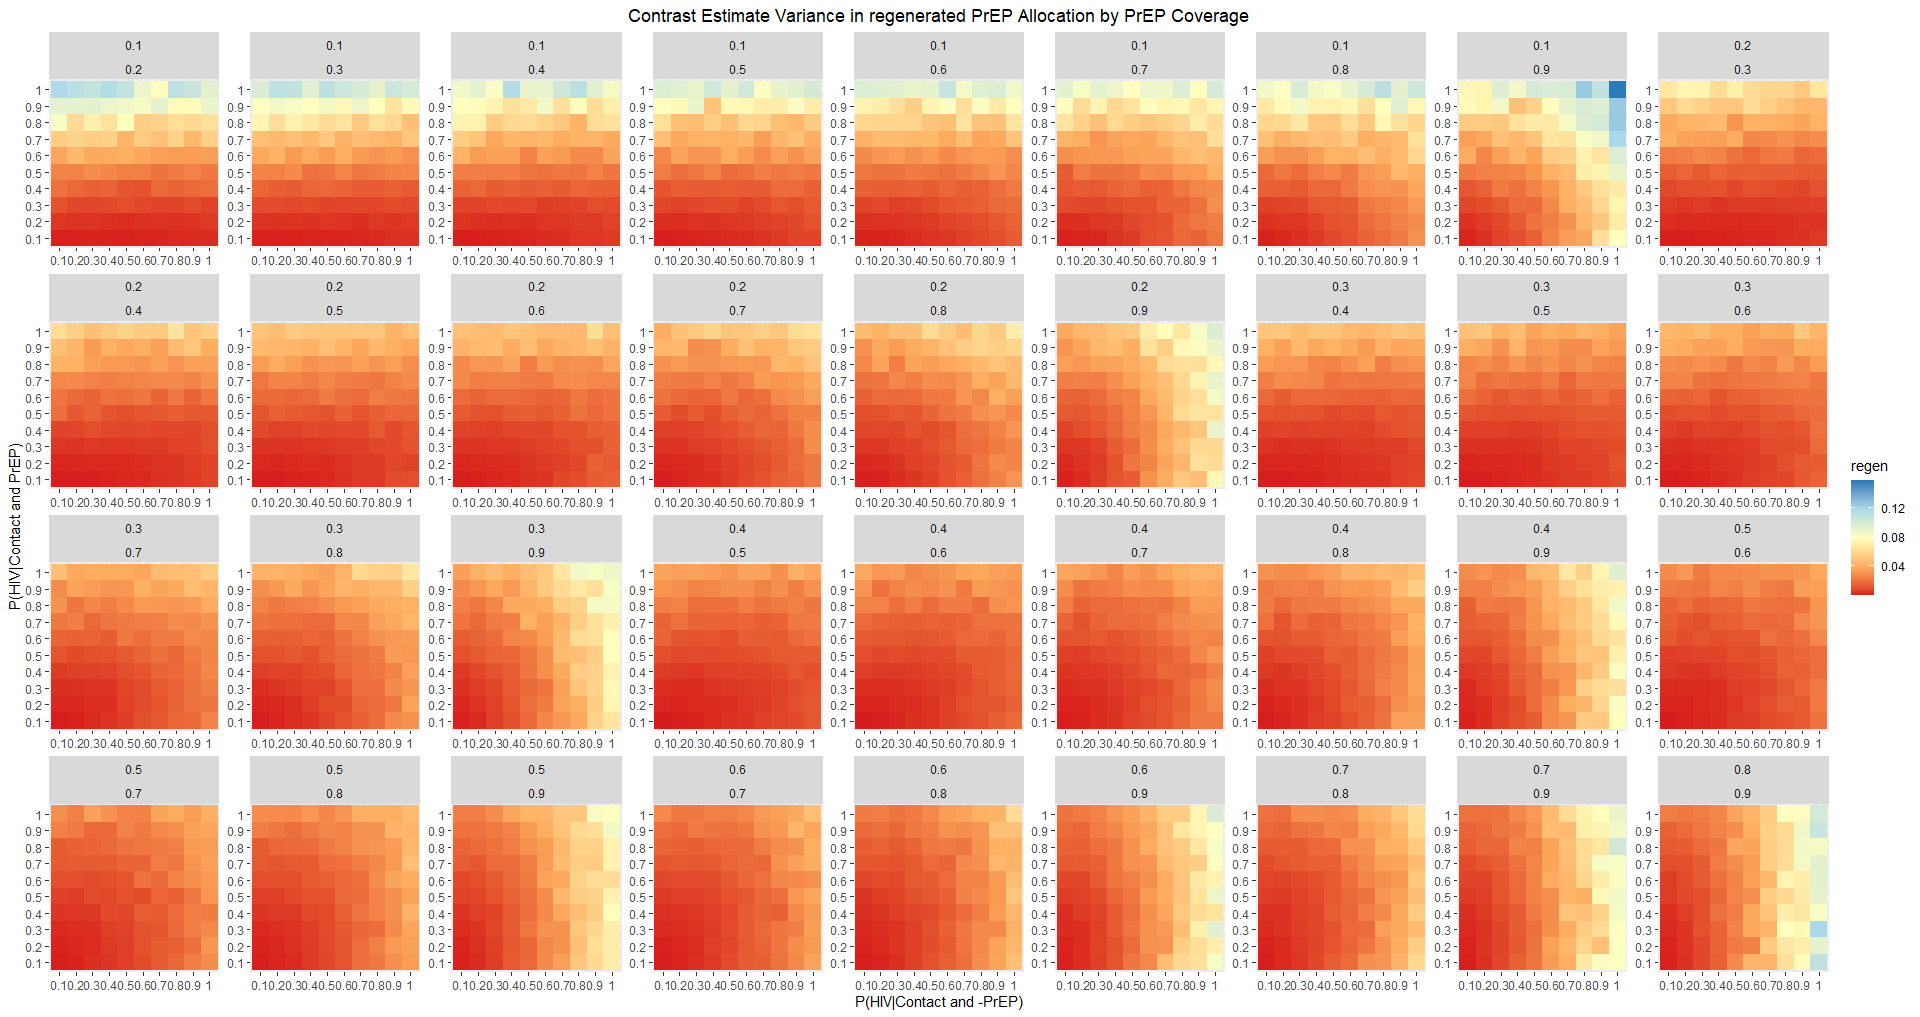
\includegraphics[width=\linewidth]{Figures/PrEP Regenerated Variance Plots.png}
    \caption{Variance of Causal Contrast estimates as $\mathbb{P}\left[\text{HIV} \vert \neg \text{PrEP} \cap \text{Contact}\right]$ and $\mathbb{P}\left[\text{HIV} \vert \text{PrEP} \cap \text{Contact}\right]$ increase, stratified by random PrEP1 \% allocation vs random PrEP2\% allocation on a regenerated network. Top number indicates PrEP1/control coverage. Bottom number is PrEP2 counterfactual coverage. }
    \label{fig:Figure 22}
\end{figure}

We can observe from the Causal Contrast Mean and Variance plots in Figures \ref{fig:Figure 17}-\ref{fig:Figure 22} that there is effect modification of the relationship between underlying HIV risks and treatment strategy by the choices of PrEP treatment contrasts. This modification is easier to identify in the Variance plots, as once again the variances for the regenerated allocation strategy contrasts display a completely different gradient across underlying risks from the additive and random strategy for all pairs of PrEP coverages. While the gradients are more similar between the random and additive strategies, there are still clear differences in contrast Variance magnitude for given choices of PrEP coverage and HIV risks. With respect to the contrast estimate Mean, effect modification is more subtle between the random and additive strategies and more apparent when comparing these two to the regenerated strategy contrasts. 
\subsection{Other Network Models}
We also considered effect modification in two other network generating models, the Barabási–Albert scale-free graph for preferential attachment, and the Watts-Strogatz Small-World graph. The parameter values considered for these models are summarized in the table below.
\begin{center}
    \begin{tabular}{|c|c|c|}
    \hline
         Parameter & Default Value & Range Considered  \\
         \hline
         Network size $N$& 50 & Fixed \\
         \hline
         BA Preferential Attachment power ``pow" & 1 & $\left[1,2 \right]$ \\
         \hline
         WS neighborhood size ``nb" & 5 & $\Set{5,10,15,20}$ \\
         \hline
         WS rewiring probability ``rprob" & 0.05 &$\left[0.05, 0.95 \right]$ \\
         \hline
         HIV prevalence ``phiv" & 0.1 & Fixed\\
         \hline
         Control PrEP Coverage ``PrEP1" & 0.2 & Fixed\\
         \hline
         Counterfactual PrEP Coverage ``PrEP2" & 0.4 & Fixed\\
         \hline
         $\mathbb{P}\left[\text{HIV} \vert \neg \text{PrEP}\right]$ $p1$ & 0.2 & $[0.1,1]$\\
         \hline
         $\mathbb{P}\left[\text{HIV} \vert \text{PrEP}\right]$ $p2$ & 0.1 & $[0.1,1]$\\
         \hline
         Re-sampling sample size ``nsim" & 200 & Fixed\\
         \hline
    \end{tabular}
\end{center}
\subsubsection{Effect Modification by Network Generating Model with Default Parameters}
\begin{figure}[H]
    \centering
    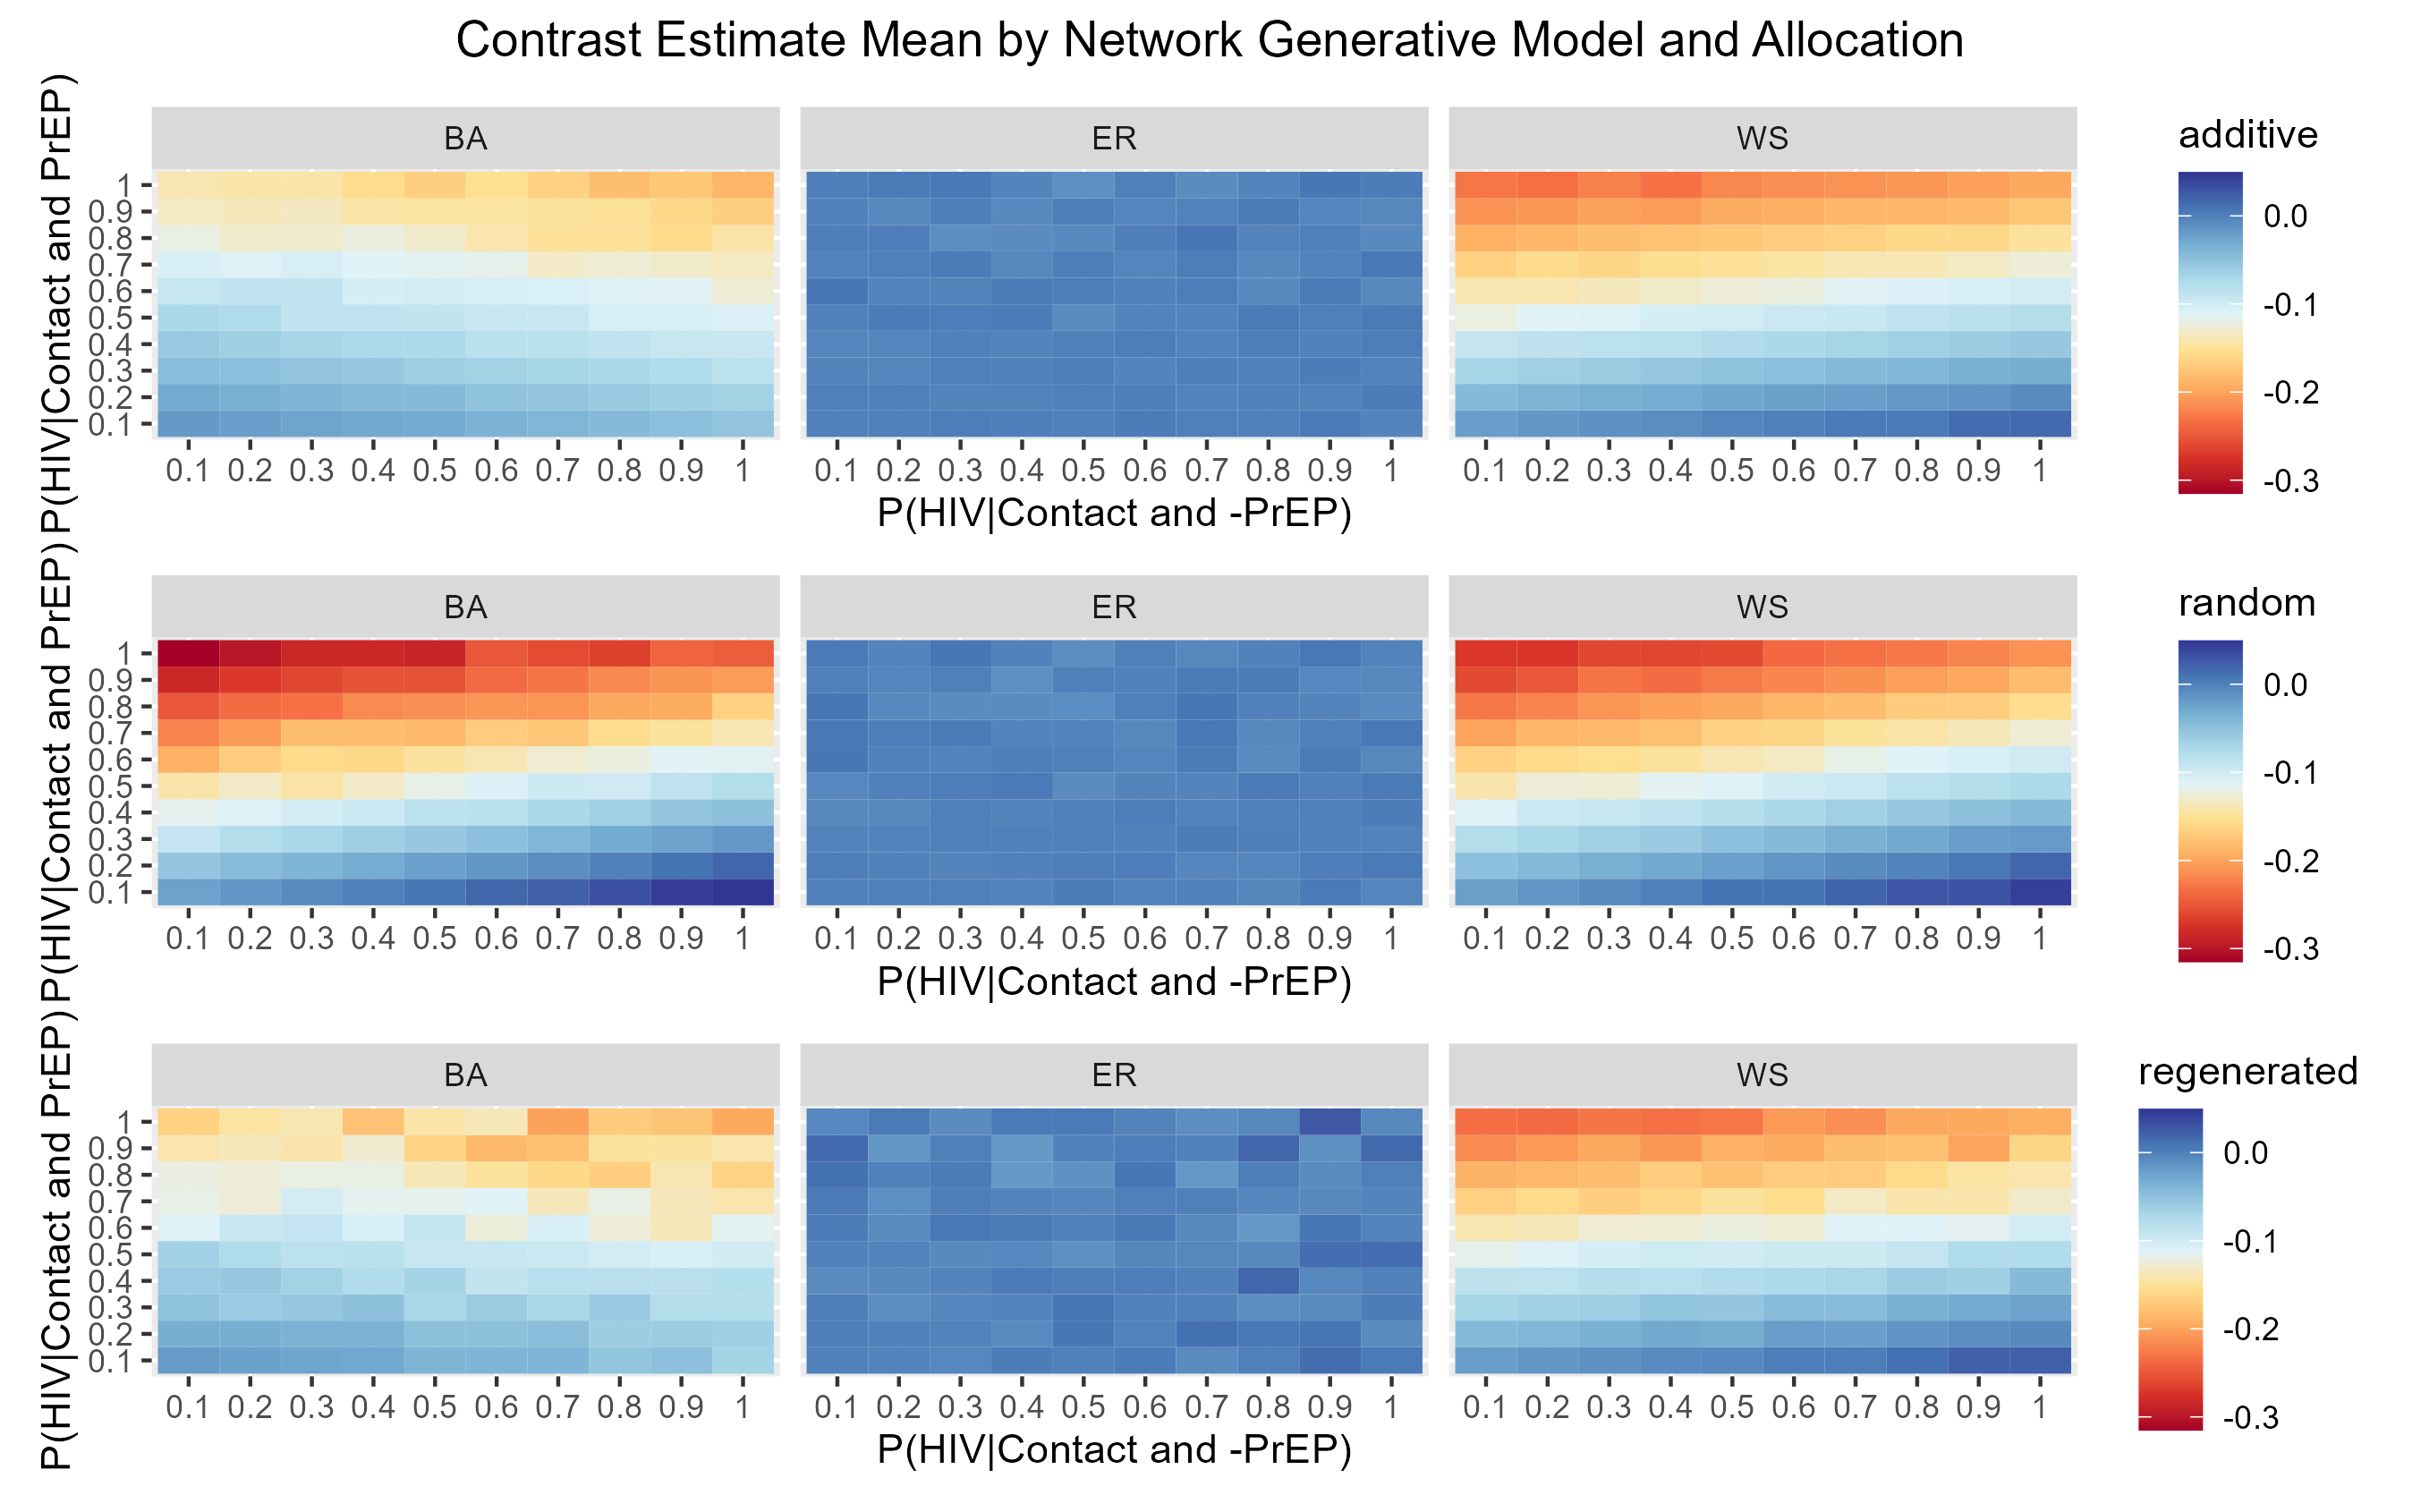
\includegraphics[width=\linewidth]{Figures/Generative Model Mean plots.png}
    \caption{Mean of Causal Contrast estimates as $\mathbb{P}\left[\text{HIV} \vert \neg \text{PrEP} \cap \text{Contact}\right]$ and $\mathbb{P}\left[\text{HIV} \vert \text{PrEP} \cap \text{Contact}\right]$ increase, stratified by stratified by the model used to generate the networks, and by estimator. From left to right, ``BA" the Barabási–Albert scale-free model, ``ER" the Erdős–Rényi Random Graph model, ``WS" the Watts-Strogatz Small-World model. From top to bottom: ``additive" Mean Contrast of random 20\% additional vs. random 20\% PrEP allocation control, ``random" Mean Contrast of random 40\% PrEP allocation vs. random 20\% control, ``regenerated" Mean Contrast of random 40\% allocation on regenerated network vs. random 20\% control. }
    \label{fig:Figure 23}
\end{figure}
From the Causal Contrast Mean plots in Figure \ref{fig:Figure 23} above, we can see stark effect modification of the relationship between underlying HIV risks and treatment strategy by the choice of network generative model. In particular, the ER model displays a completely different gradient than those of the BA or WS models for all treatment strategies. There is also a ``reversal" in the direction of effects for the BA model with random allocation compared to additive and regenerated strategies, as well as relatively large differences in magnitude of effect estimates. WS model effect estimate magnitudes are also different across treatment strategies. 

\begin{figure}[H]
    \centering
    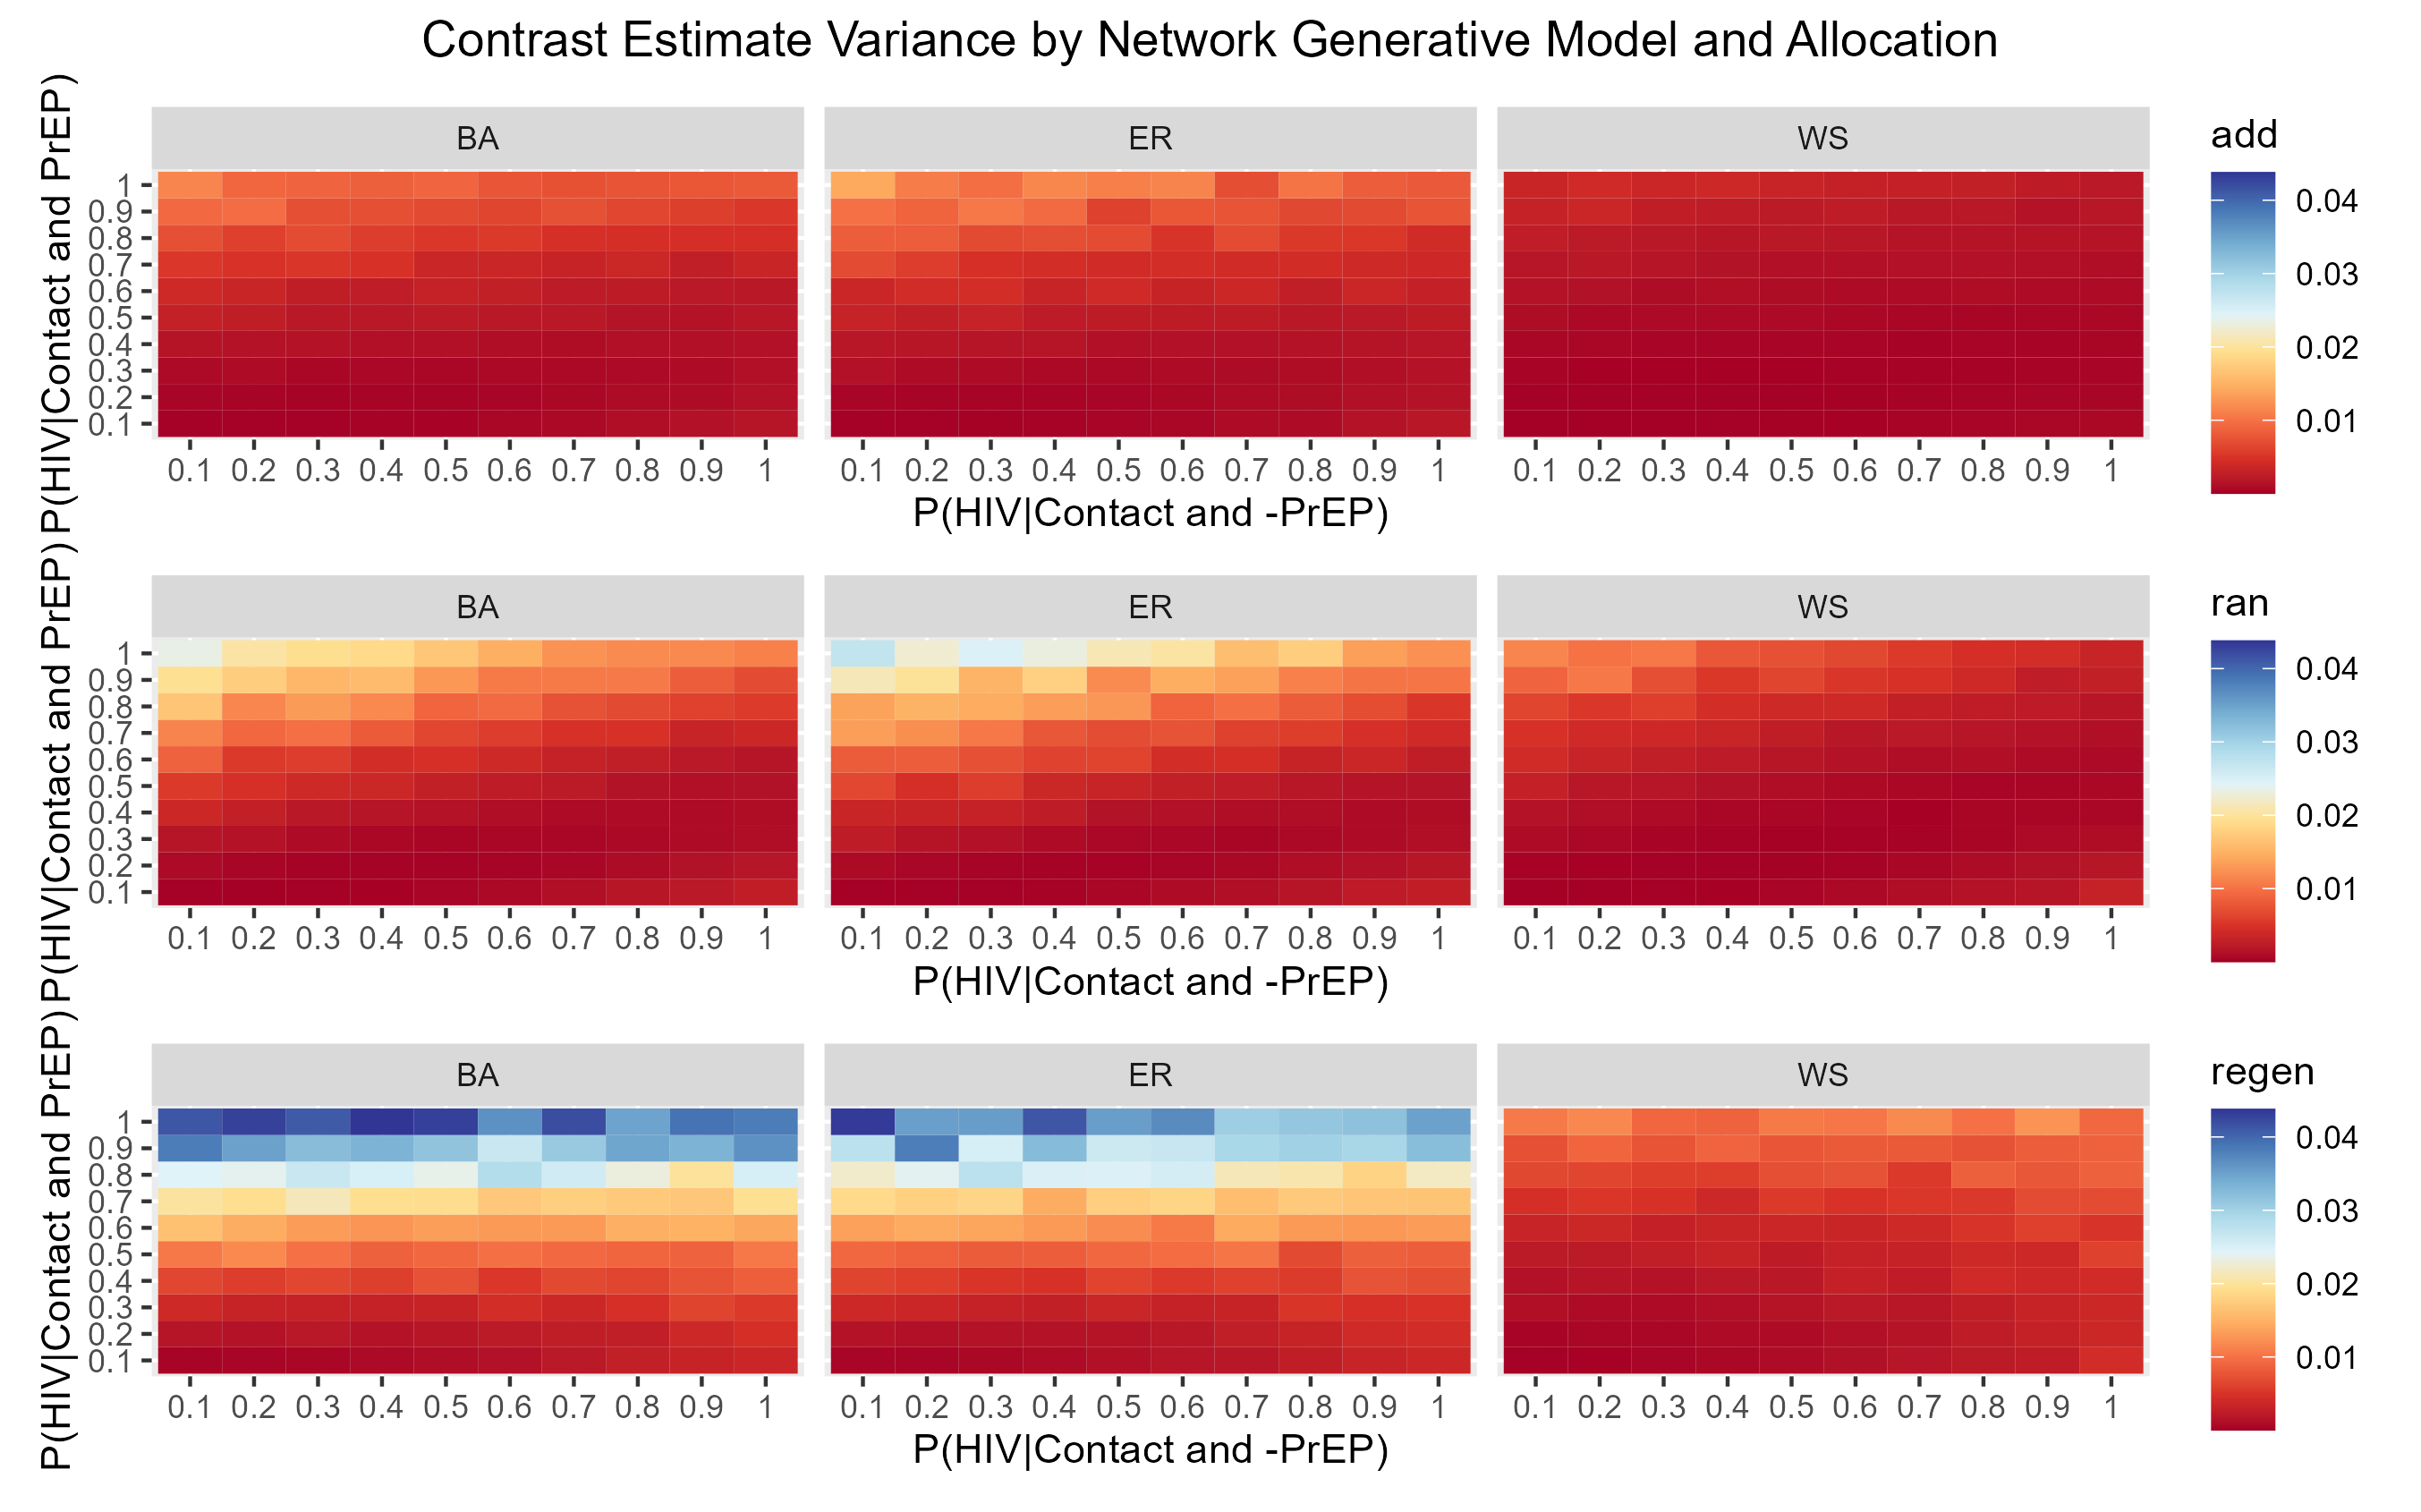
\includegraphics[width=\linewidth]{Figures/Generative Model Variance plots.png}
    \caption{Variance of Causal Contrast estimates as $\mathbb{P}\left[\text{HIV} \vert \neg \text{PrEP} \cap \text{Contact}\right]$ and $\mathbb{P}\left[\text{HIV} \vert \text{PrEP} \cap \text{Contact}\right]$ increase, stratified by stratified by the model used to generate the networks, and by estimator. From left to right, ``BA" the Barabási–Albert scale-free model, ``ER" the Erdős–Rényi Random Graph model, ``WS" the Watts-Strogatz Small-World model. From top to bottom: ``additive" Variance of Contrast of random 20\% additional vs. random 20\% PrEP allocation control, ``random" Variance of Contrast of random 40\% PrEP allocation vs. random 20\% control, ``regenerated" Variance of Contrast of random 40\% allocation on regenerated network vs. random 20\% control.}
    \label{fig:Figure 24}
\end{figure}
The Causal Contrast Variance plots in Figure \ref{fig:Figure 24} above also clearly show effect modification  of the relationship between underlying HIV risks and treatment strategy by the choice of network generative model.  Interestingly, the Variance gradients appear similar across models in the ``additive" allocation strategy. While the magnitudes of Variance estimates vary slightly, the gradient for the Watts-Strogatz model is much more consistent  across allocation strategies than for the Barabási–Albert or  Erdős–Rényi models. In particular, the gradients within these two models are markedly different by allocation strategy, although the pattern of changes is similar between these models across strategies.  

\section{Discussion}

For all model parameters considered, there is clear effect modification of the relationship between risks of HIV given infectious contact with and without PrEP treatment. This modification is apparent for all parameters in both means and variances of Causal Contrast estimates.

Of particular interest is the stark effect modification by the choice of network generative model.  For both contrast Means and Variances, the dramatically different gradients and magnitudes across underlying risks demonstrate that the effect estimates are highly sensitive to the choice of allocation when the network structure changes, i.e., network structure clearly modifies treatment effect estimates under differing allocation strategies. When repeated with fixed parameters and larger network sizes, the relationships observed for the Barabási–Albert and Erdős–Rényi Network models were relatively robust, but relationships for all Watts-Strogatz models attenuated, indicating possible interaction between network model parameters in modifying the estimate relationships (see .

Some other observed modification is perhaps unsurprising, such as that observed here for Network Size and Resampling sample size. It is expected (but important) that variance estimates appear to converge for sufficiently large resampling sizes, thus small resampling sizes may provide inconsistent/unreliable characterizations of the effect estimate distribution.
Combinatorial results suggest that the effect estimates should tend toward the null as network sizes grow sufficiently large (see section \ref{sec: Treat}, Appendix \ref{sec:A}). Simulation results presented here for the  Erdős–Rényi Random Graph model are consistent with this, at least across one order of magnitude. Larger magnitudes could not be implemented due to computational constraints.

While the exact nature and implications of the effect modification observed in effect estimates under changing pairs of PrEP coverages seen here is difficult to describe (i.e, modified relationships are difficult to interpret), it is nonetheless clear that both the contrast estimate  means and variances are modified by these coverage choices under changing treatment allocation strategy. Thus, the exact choice of counterfactual treatment levels is an important consideration for networked designs. 


Also of interest is the apparent effect modification by the underlying risk parameters. Since for both $\mathbb{P}\left[\text{HIV } \vert \text{ PrEP}\right]$ and $\mathbb{P}\left[\text{HIV} \vert \neg \text{PrEP}\right]$ the estimate variances have different relationships with underlying risk between allocation strategies, the choice of estimator may be important when evaluating effects of treatment assignment. These results also raise questions about the reliability/equivalence of network regeneration estimands as counterfactuals for network structure estimands (see section \ref{sec:Regen}) as there is clear heteroskedasticity in the regenerated effect estimate variances across risk parameters that is not present in the random or additive strategy variances.  
\appendix
\counterwithin{figure}{section}
\section{Definition for \textit{P}}
\label{sec:A}
Here we describe the details of the definition for $P$, the probability of at least one node $i$ in a network being assigned to treatment with at least one infectious contact for a given network structure $j$ and a given treatment $a$ or $a*$

Assume as before that $N$ is the network population at a given time point, that $k<N$ is the number of individuals that receive treatment, and that $n<N$ is the number of individuals with an infectious contact.

 Then, there are $\binom{N}{k}$ unique network configurations.
 
The expected number of unique network configurations in which all treated individuals have no infectious contacts (and thus a contribution of 0 to the effect estimate) is then given by $\binom{N-n}{k}$. Then, the proportion of network configurations in which at least one treated individual has at least one infectious contact is 
\begin{equation} 
\frac{{\binom{N}{k}}-{\binom{N-n}{k}}}{{\binom{N}{k}}}=1-\frac{{\binom{N-n}{k}}}{{\binom{N}{k}}}    
\end{equation}
Expanding the RHS gives:
\begin{equation}
1-\frac{\left(N-n\right)!\left(N-k\right)!}{k!\left(N-n-k\right)!}
\end{equation}
Using Stirling's Approximation as appropriate,
\begin{equation}
\approx 1-\frac{\sqrt{2\pi\left(N-n\right)}\left(\frac{N-n}{e}\right)^{N-n}\sqrt{2\pi\left(N-k\right)}\left(\frac{N-k}{e}\right)^{N-k}}{\sqrt{2\pi N}\left(\frac{N}{e}\right)^{N}\sqrt{2\pi \left(N-n-k\right)}\left(\frac{N-n-k}{e}\right)^{N-n-k}}    
\end{equation}
%see page 2b
We can then make the following approximations and simplifications:
\begin{equation}
    \frac{\sqrt{2\pi \left(N-n\right)}}{\sqrt{2\pi N}}=\sqrt{\frac{N-n}{N}}\approx 1 \text{ for } N>>n\\
    \end{equation}
    \begin{equation}
    \frac{\sqrt{2 \pi \left(N-k\right)}}{\sqrt{2 \pi \left(N-n-k\right)}}\approx 1
\end{equation}
    \begin{align}
    \frac{\left(\frac{\left(N-n\right)}{e}\right)^{N-n}}{{\left(\frac{N}{e}\right)^{N}}}&=\frac{\left(N-n\right)^{N-n}e^{N}}{N^{N}e^{N-n}}\\
     &=\frac{e^{n}}{N^{n}}\left(\frac{N-n}{N}\right)^{N-n}\\
     &=\frac{e^{n}}{N^{n}}\left(1-\frac{n}{N}\right)^{N-n}\\
     &=\frac{e^{n}}{N^{n}}\frac{\left(1-\frac{n}{N}\right)^{N}}{\left(1-\frac{n}{N}\right)^{n}}\\
     &\approx \frac{e^{n}}{N^{n}}\lim_{N \to \infty}\frac{\left(1-\frac{n}{N}\right)^{N}}{\left(1-\frac{n}{N}\right)^{n}}\\
     &=\frac{e^{n}}{N^{n}}\frac{e^{-n}}{1^{n}}\\
     &=\frac{1}{N^{n}}
\end{align}
\begin{align}
    \frac{\left(\frac{N-k}{e}\right)^{N-k}}{\left(\frac{N-n-k}{e}\right)^{N-n-k}}&\stackrel{M\coloneqq N-k}{=}\frac{\left(\frac{M}{e}\right)^{M}}{\left(\frac{M-n}{e}\right)^{M-n}}\to M^{n}\\
    \frac{M^{n}}{N^{n}}&=\left(\frac{N-k}{N}\right)^{n}
\end{align}
simplifying as appropriate gives
\begin{align}
    & \approx 1- \frac{\left(N-n\right)^{N-n}\left(N-k\right)^{N-k}}{N^{N}\left(N-n-k\right)^{N-n-k}}\\
    &= 1- N^{-N}\left(\frac{N-n}{N}\right)^{N-n}\left(N-k\right)^{n}\left(\frac{N-k}{N-n-k}\right)^{N-n-k}\\
    &=1-\left(\frac{N^{n}\left(1-\frac{n}{N}\right)^{N}\left(N-k\right)^{n}}{\left(1-\frac{n}{N}\right)^{n}}\right)\left(\frac{N-n-k}{N-k}\right)^{k+n-N}\\
    &=1-\left(\frac{N^{-n}e^{-n}\left(N-k\right)^{n}}{1}\right)\left(\frac{\left(1-\frac{n}{N-k}\right)^{n}}{\left(1-\frac{n}{N-k}\right)^{N-k}}\right)\\
    &=1-\frac{N^{-n}\left(N-k\right)^{n}e^{-n}}{e^{-n}}\\
    &=1-\frac{\left(N-k\right)^{n}}{N^{n}}\\
    &=1-\left(\frac{N-k}{N}\right)^{n}.
\end{align}
\section{Summary Statistics}
\subsection{Definitions}
\begin{definition}[Connected Components]
A connected component of a graph $G=(V,E)$ is a subgraph $G'=(V' \subseteq V,E' \subseteq E)\subseteq G$ such that there exists a path between any two nodes in $V'$.
\end{definition}
\begin{definition}[Betweenness Centrality]
The Betweenness Centrality for a node $v$ is given by: $$g(v)=\sum_{s\neq t\neq v}\frac{\sigma_{s,t}(v)}{\sigma_{s,t}},$$ where $\sigma(s,t)$ is  the number of shortest paths between node s and node t, and  $\sigma_{s,t}(v)$ is the number of shortest paths between node $s$ and node $t$ containing the node $v$ \cite{barabasi_network_2016}.
\end{definition}
\begin{definition}[Edge Density]
The (edge) density of a graph is the proportion of possible edges between nodes
that are actually present in the graph.
\end{definition}
\begin{definition}[Geodesic distance]
The geodesic distance between two nodes is the length of the shortest path between them.
\end{definition}
\begin{definition}[Graph diameter]
The diameter of a graph or graph component is the largest path length between any two nodes is the graph (component).
\end{definition}
\begin{definition}[Transitivity]
Transitivity is the proportion of closed triangles in a graph.
\end{definition}
\begin{definition}[$k$-core decomposition]
A $k$-core of a graph is a subgraph in which all nodes are connected to at least $k$ other nodes in the subgraph.
\end{definition}
\subsection{Results by Network Model}
\begin{figure}[H]
    \centering
    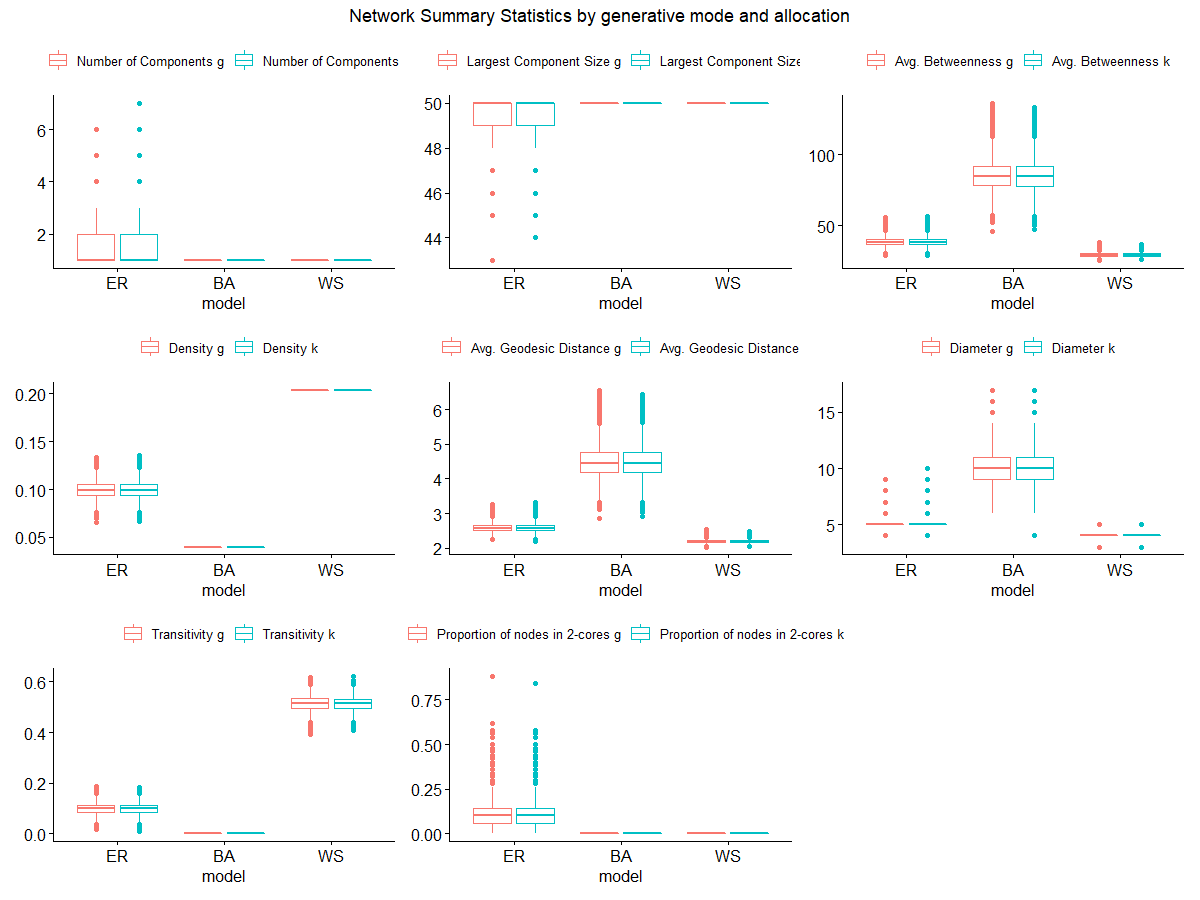
\includegraphics[width=\linewidth
    ]{Figures/Network Summary Statistics.png}
    \caption{Select Network Summary Statistics by Network Generative Model}
    \label{fig:Figure B1}
\end{figure}
% \section{Expanded Effect Definitions}

% \subsection{Overall Effect}
%As before,  let $Y$ be the outcome of interest, $a$, $a∗$ be counterfactuals of treatment strategy $A$, and $j$ be an identifier of a network.
% The Overall Effect (OE) at timestep $t$ of counterfactual PrEP allocation $a>a*$ is the difference of the marginal population average potential outcomes under $a$ and $a*$:
% \begin{equation}
%     OE(a)=\mathbb{E} [Y_{t}^{a}]-\mathbb{E}[Y_{t}^{a*}].
% \end{equation}
\section{Example Annotated Networks for all Generative Models}
\begin{figure}
    \centering
    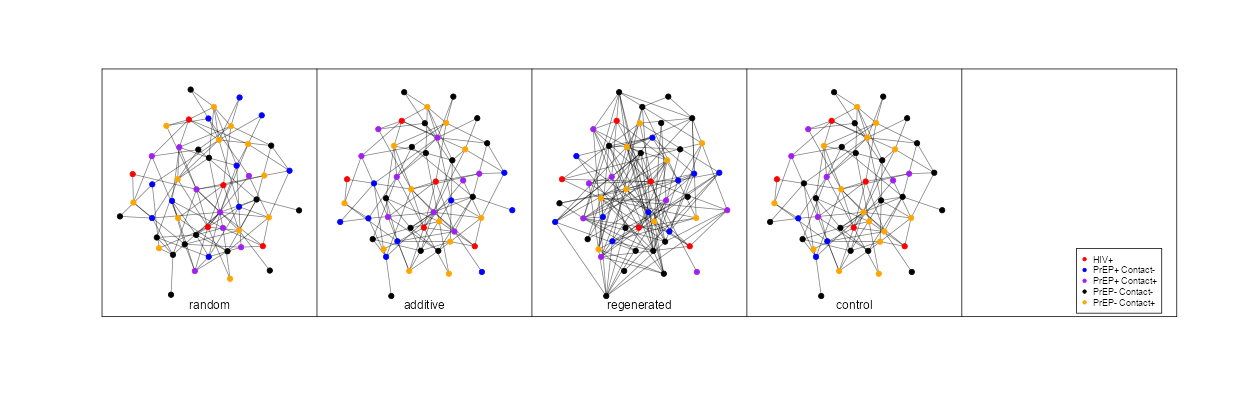
\includegraphics[width=\linewidth]{Figures/ER Network Example.png}
    \caption{Annotated Example ER Network showing color-coded treatment and disease states by network (control vs. regenerated) and allocation strategy(control vs. random, additive)}
    \label{fig: C1}
\end{figure}
\begin{figure}[H]
    \centering
    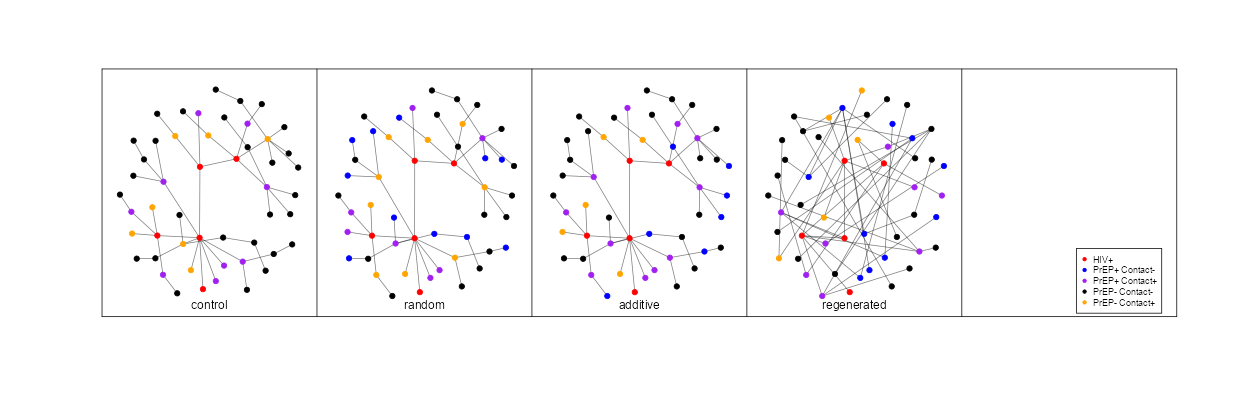
\includegraphics[width=\linewidth]{Figures/BA Network Example.png}
    \caption{Annotated Example BA Network showing color-coded treatment and disease states by network (control vs. regenerated) and allocation strategy(control vs. random, additive)}
    \label{fig: C2}
\end{figure}
\begin{figure}[H]
    \centering
    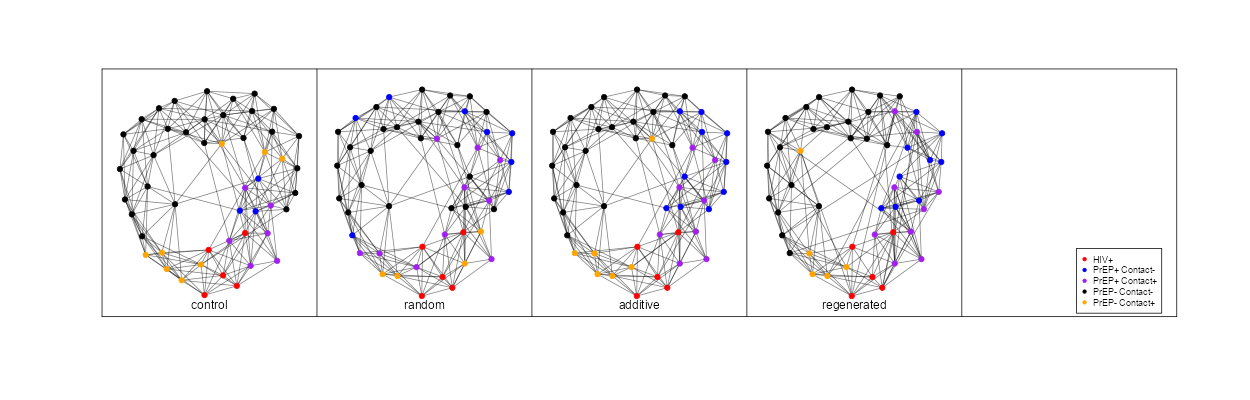
\includegraphics[width=\linewidth]{Figures/WS Network Example.png}
    \caption{Annotated Example WS Network showing color-coded treatment and disease states by network (control vs. regenerated) and allocation strategy (control vs. random, additive)}
    \label{fig: C3}
\end{figure}
\section{Results by Network Generative Model with Larger Network Size}
\label{sec: D}
\begin{figure}
    \centering
    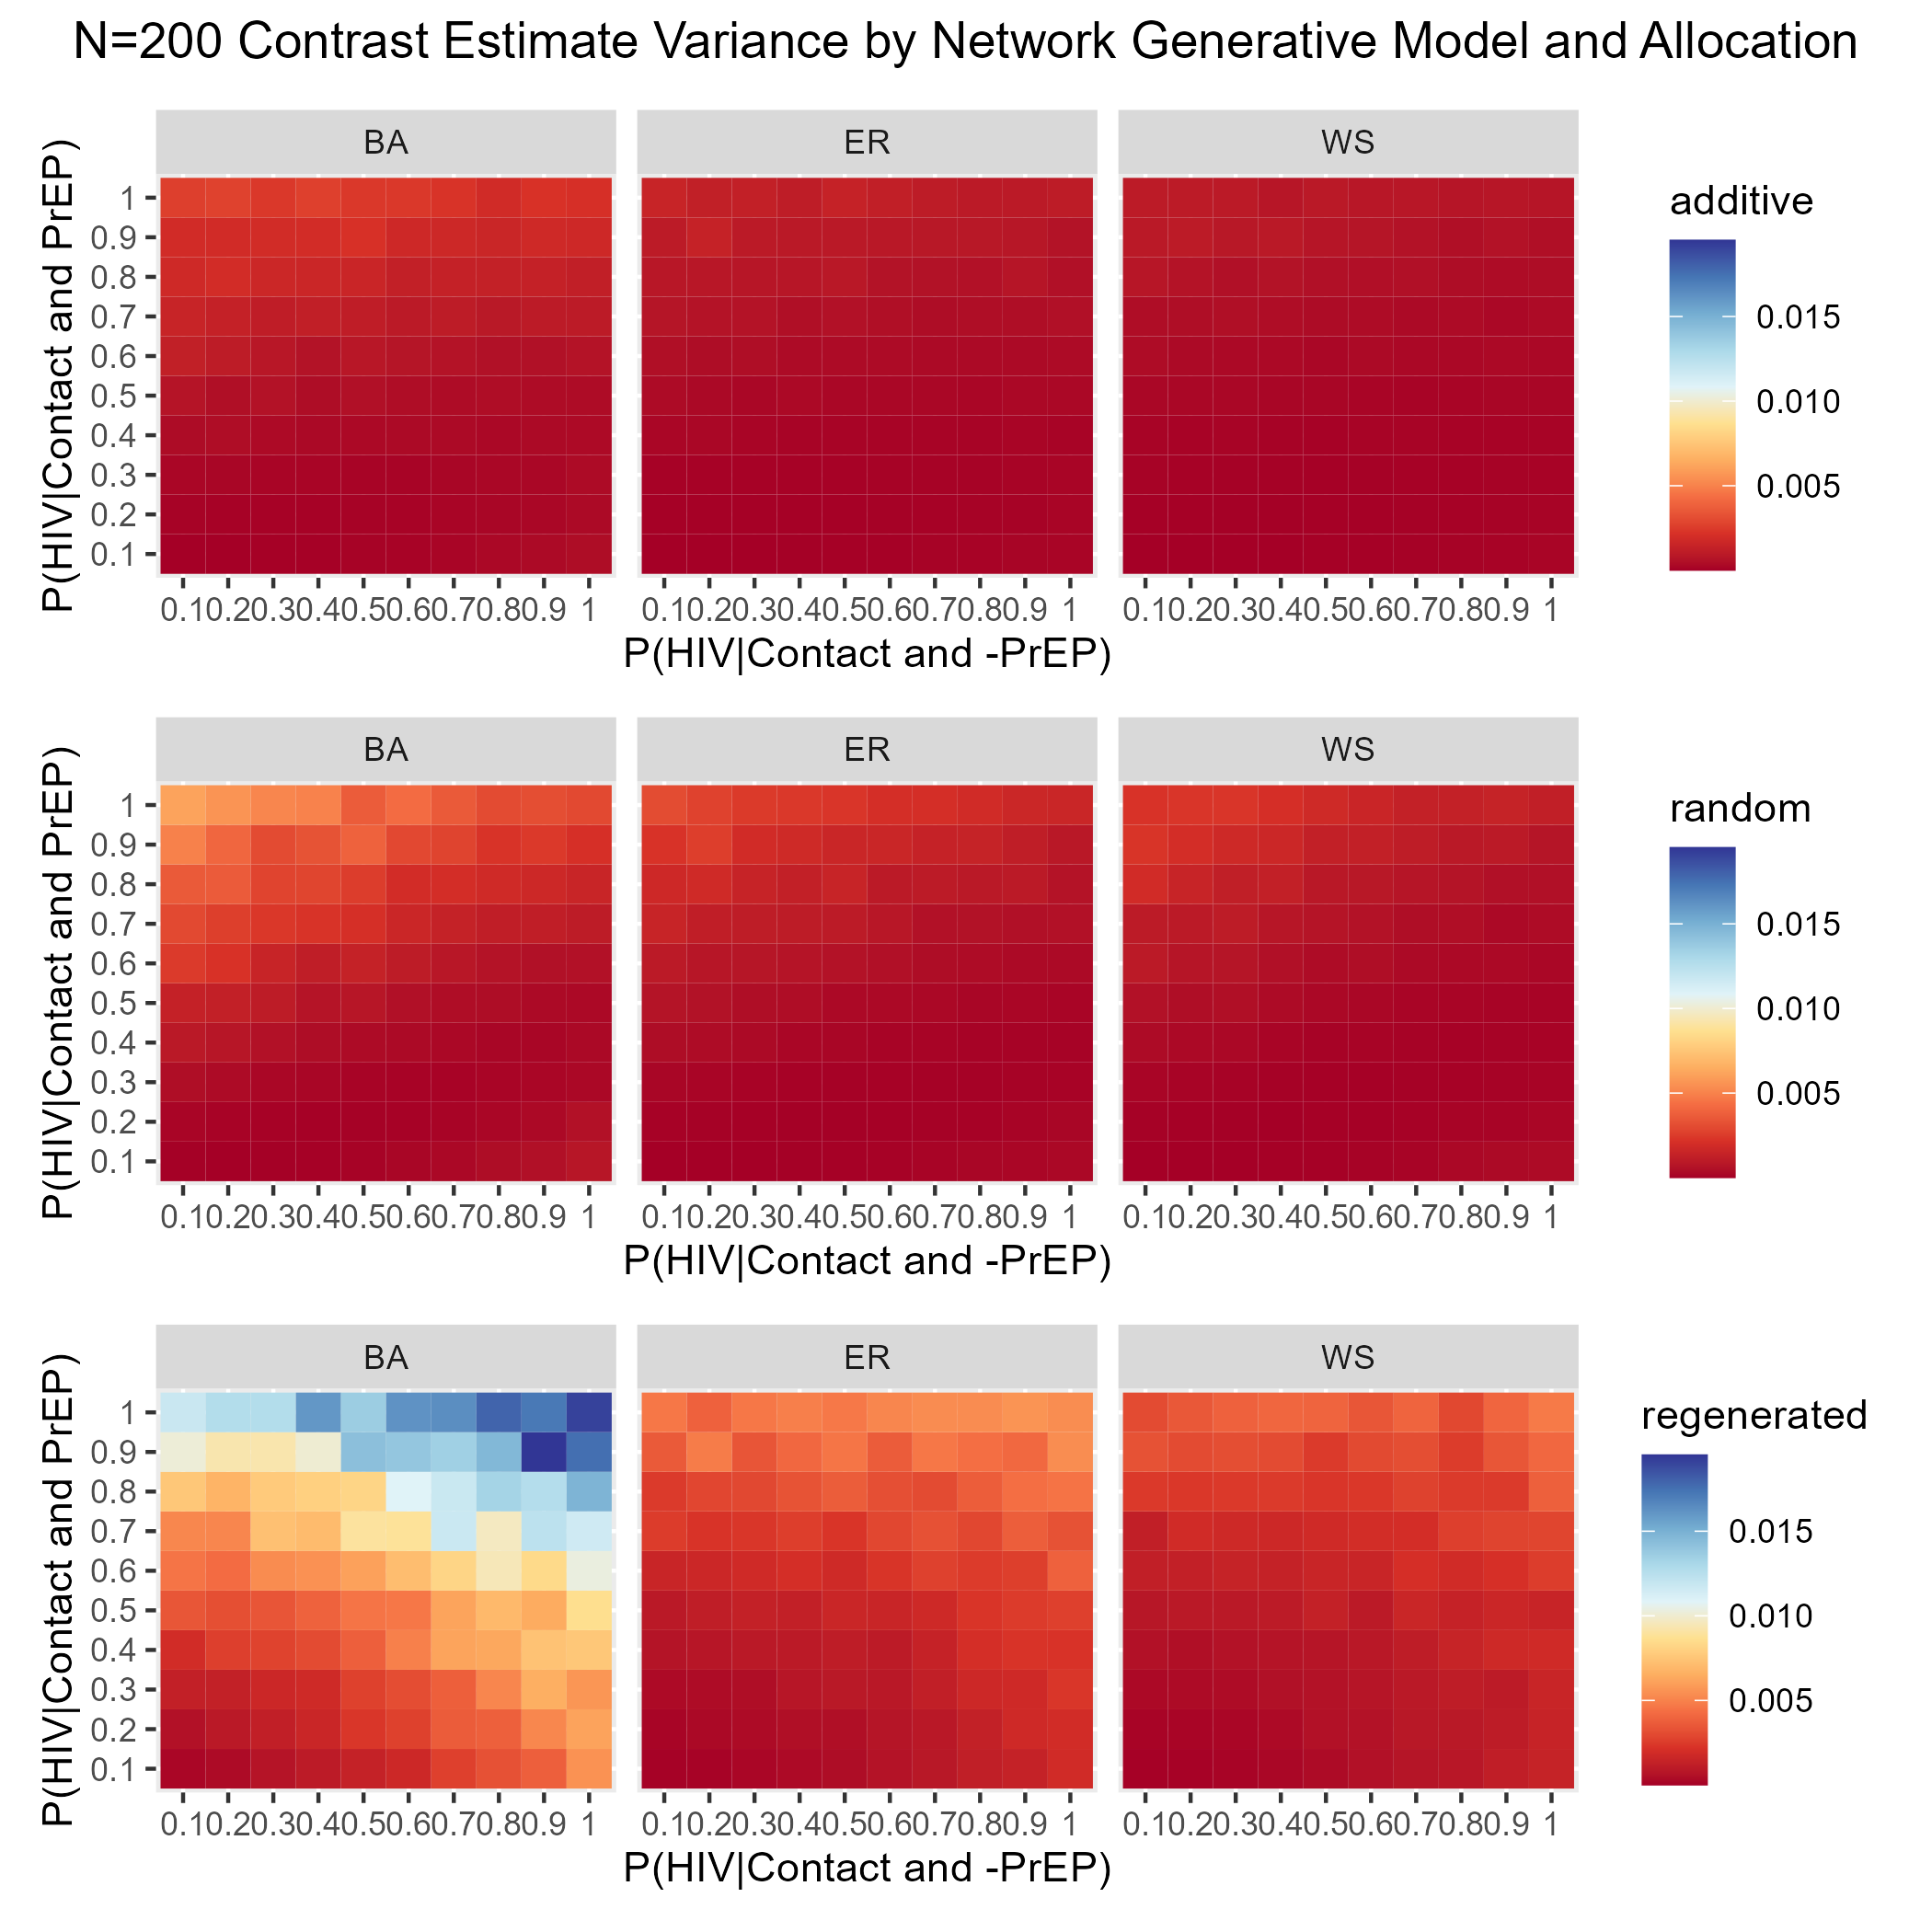
\includegraphics{Figures/N=200 Generative Model Variance plots.png}
    \caption{Caption}
    \label{fig:my_label}
\end{figure}
\bibliographystyle{unsrt}
\bibliography{references}
\end{document}